\chapter{Analysis Strategy}%
\label{ch:strategy}

With the objects required for this analysis reconstructed and an event selection
in place an analysis strategy is formed in order to maximise the signal strength
of the \VHbb\ process and yield a robust result that is well understood in terms
of modelling and systematic errors. The data the analysis strategy is executed
on is 140 fb${^-1}$ of proton-proton collision data recorded by the ATLAS
detector at a centre of mass energy of $\sqrt{s} = 13$~\TeV\ during Run 2 of the
LHC (2015--2018). Data and Monte Carlo predictions are grouped into datasets
called mc16a, mc16d and mc16e that refer to data taken in the periods
2015--2016, 2017 and 2018 respectively.

First the categorisation into analysis regions will be defined, then the
composition of those regions will be explained detailing the simulated samples
used, next the multi-variate algorithm that is used to generate some of the
distributions entering into the profile-likelihood fit will be explained. Then
the fit itself will be explained, including a definition of the likelihood
function and systematic uncertainty model. Plots of the data versus Monte-Carlo
prediction will then be shown in order to build a picture of the pre-fit status
of the agreement. Finally a series of cross-checks which are used to validate
the methods of the analysis will be explained.

The author's contributions include studying the behaviour of the
profile-likelihood fit with the inclusion of these regions, which are new in
this round of the analysis and making comparisons between the 80~fb$^{-1}$ and
140~fb$^{-1}$ datasets). Contributions also include the training of the
multi-variate classification algorithm with the inclusion of new input variables
with respect to the previous version of the algorithm.

\section{Categorisation Into Analysis Regions}
\label{sec:ana-regions}

Events which pass the selection detailed in table~\ref{tab:event-selection} are
categorised into several regions for analysis. Firstly they are split into what
are known as medium (75--150~\GeV), high (150--250~\GeV) and extreme (>250~\GeV)
$p_{\mathrm{T}}^{V}$. Events are further categorised by jet multiplicity, all
jets are required by the selection to have at least two jets, categories are
defined for events with exactly two, or exactly three jets. In the 2--lepton
channel there is a requirement of three or more jets but when referring to all
three channels at once categorisation is referred to as simply 3--jet or 2--jet.

Events are categorised into a signal region which is straddled either side by
two control regions. This categorisation is achieved via cuts defined in the
$\Delta R(b, \bar{b})$~--~$p_{\mathrm{T}}^{V}$ plane, they are chosen to
maximise the signal purity in the signal region and are shown for the 1--lepton
channel in figure~\ref{fig:drbb-crs}, and come from a previous iteration of the
analysis that did not use a machine learning based classifier. In this iteration
of the analysis~\cite{ObsHbbInternal} the cuts were originally optimised to
yield a control region pure in $W + hf$ events (which had ~75\% purity), and
have been adapted to allow for a single set of cuts which can be used in all
channels of the analysis in the di-jet mass fit, as well as the multi-variate
fit.
\begin{figure}[h]
  \centering
  \begin{tabular}{cc}
    \subfloat[]{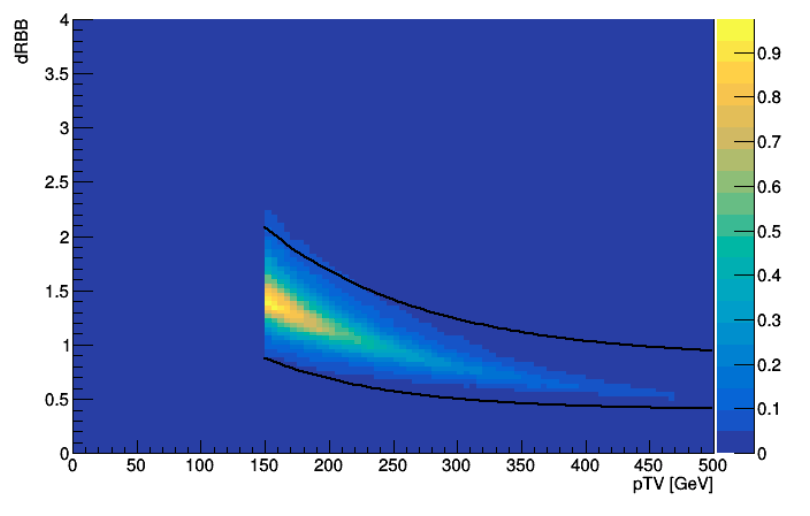
\includegraphics[width=0.505\linewidth]{1lep_qqWH_2tag_2jet.png}}
    \subfloat[]{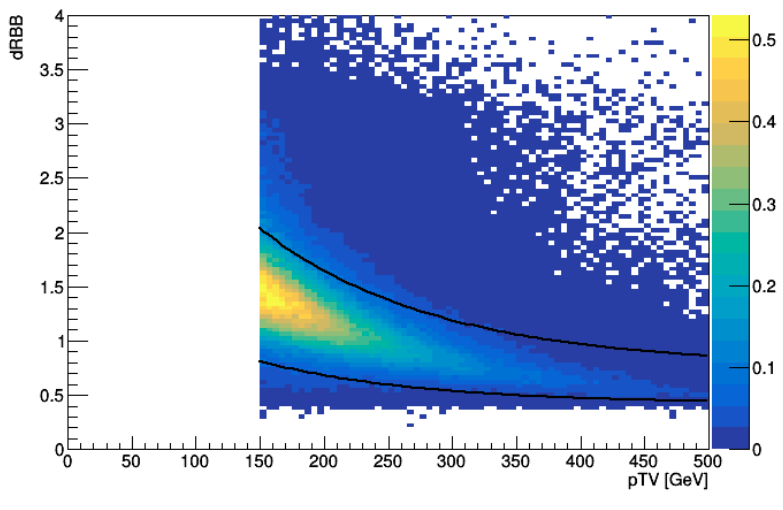
\includegraphics[width=0.49\linewidth]{1lep_qqWH_2tag_3jet.png}}\\
  \end{tabular}
  \caption{Signal distribution of $\Delta R$ between the two selected jets as
    function of $p_{T}^{V}$ in the 1-lepton channel are shown in the 2-tag 2-jet
    (a) and 2-tag 3-jet (b) categories. The black lines demonstrate the upper
    and lower continuous cuts used to categorise the events into the signal and
    control regions}
  \label{fig:drbb-crs}
\end{figure}
The regions either side of the signal region are known as the high-$\Delta R(b,
\bar{b})$ and low-$\Delta R(b, \bar{b})$ control regions, shortened to
CR$_{\text{high}}$ and CR$_{\text{low}}$ respectively.

\subsection{Top \texorpdfstring{$e \mu$}{e mu} Control Region}%
\label{sec:topemucr}

One more region exists only in the 2--lepton channel, it is obtained by
requiring two opposite flavour leptons instead of two same flavour leptons, and
keeping all other selection criteria the same. This region consists almost
entirely of $t\bar{t}$ and single top processes (whose Feynman diagrams belong
to the same sum) matching very closely the number of expected events of each of
these backgrounds in the 2--lepton channel. This region is therefore called the
top $e \mu$ control region. The data from this control region can be used as a
prediction for the number of top process events in the 2--lepton channel once
multiplied by a scale factor which accounts for differences in normalisation.
Given that this region exists purely to model systematic uncertainties it will
explored in more detail in the subsequent chapter in section~\ref{sec:ttbar_DD}.

\section{Composition of Analysis Regions}
\label{sec:composition}

This section will detail the composition of each analysis region in terms of
background and signal processes. For all regions the signal process is \VHbb,
the prediction for which comes from events generated using \textsc{Powheg
MiNLO}~\cite{Luisoni2013}~+~\textsc{Pythia~8}~\cite{pythia8} for quark initiated
processes and \textsc{Powheg}~+~\textsc{Pythia~8} for gluon initiated processes
as can be seen in table~\ref{tab:sigMC}. \begin{table}[tbph]
\centering
\resizebox{\textwidth}{!}{
  \begin{tabular}{llrS[table-format=3.2]S[table-format=3.2]S[table-format=3.2]}
    \toprule
    {\bfseries Process} & {\bfseries Generator} & \bfseries{$\bm{\sigma \times BR}$ [pb]} & \multicolumn{3}{c}{{\bfseries $\bm{N_{\text{events}}}$ in millions}}\\
                        &&&\bfseries{mc16a}&\bfseries{mc16d}&\bfseries{mc16e}\\
    \midrule

    $qq \to ZH \to \nu\nu b\bar{b}$ & \textsc{Powheg MiNLO} + \textsc{Pythia 8 } (NNPDF3)& $153.05\times0.582$ & 2  & 2  & 3.3  \\
    $qq \to WH \to l^+\nu b\bar{b}$ & \textsc{Powheg MiNLO} + \textsc{Pythia 8 } (NNPDF3)& $282.78\times0.582$ & 4  & 4  & 6.6  \\
    $qq \to WH \to l^-\nu b\bar{b}$ & \textsc{Powheg MiNLO} + \textsc{Pythia 8 } (NNPDF3) & $179.49\times0.582$ & 2  & 2  & 3.3  \\
    $qq \to ZH \to ll b\bar{b}$ & \textsc{Powheg MiNLO} + \textsc{Pythia 8 } (NNPDF3)& $77.04\times0.582$ & 3  & 3  & 5  \\
    $gg \to ZH \to \nu\nu b\bar{b}$ & \textsc{Powheg} + \textsc{Pythia 8}  (NNPDF3) & $24.57\times0.582$ & 0.5  & 0.5  & 0.5  \\
    $gg \to ZH \to l^{-}l^{+} b\bar{b}$ & \textsc{Powheg} + \textsc{Pythia 8} (NNPDF3) & $12.42\times0.582$ & 0.75  & 0.75  & 0.75  \\
\bottomrule
\end{tabular}
}
\caption{Monte Carlo samples used for the signal processes and the cross section
  and branching ratio (BR) used to normalise the different processes at
  $\sqrt{s}=13$~TeV. Branching ratios correspond to the $H\rightarrow b\bar{b}$
  decay while $V$ branching ratio are still included in the cross-section. This
  was made to make easier the comparison with the reference tables computed
  including $V$ decays in~\cite{twikiCrossSections}. $l$ corresponds to all $e$,
  $\mu$ and $\tau$ leptons together.}
\label{tab:sigMC}
\end{table}


The 0--lepton channel contains the $Z + $jets, $W+$jets, top quark and diboson
backgrounds. The $Z+$jets background dominates the mixture in the 2--jet
category across signal and control regions. In the 3--jet category the top-quark
processes dominate apart from in CR$_{\text{low}}$. There is very little signal
contamination in the control regions. As can be seen in table~\ref{tab:bkgMC},
$V+$jets events are generated using \textsc{Sherpa~2.2.1}, top quark events are
generated using \textsc{Powheg}~+~\textsc{Pythia~8} and diboson events are
generated also using \textsc{Sherpa~2.2.1}, this is true for these backgrounds
across all channels where a Monte-Carlo prediction is used.
\begin{table}[tbph]
\centering
\resizebox{\textwidth}{!}{
  \begin{tabular}{lllrrrr}
    \toprule
    \multicolumn{2}{l}{{\bfseries Process}} & {\bfseries Generator} & \bfseries{$\bm{\sigma \times BR}$ [pb]} & \bfseries{$\bm{N_{\text{events}}}$ (mc16a)} & \bfseries{$\bm{N_{\text{events}}}$ (mc16d)} & \bfseries{$\bm{N_{\text{events}}}$ (mc16e)}\\
    \midrule
    \multicolumn{2}{l}{\bfseries{Vector boson + jets}} & & & & & \\
    \multicolumn{2}{l}{$Z \to \nu\nu$} & \textsc{Sherpa} $2.2.1$ & $56280\times0.200$ & 150M & 160M & 140M \\
    \multicolumn{2}{l}{$W \to \ell\nu$} & \textsc{Sherpa} $2.2.1$ & $183600\times0.325$ & 340M & 400M & 540M \\
    \multicolumn{2}{l}{$Z/\gamma^{*} \to \ell\ell$} & \textsc{Sherpa} $2.2.1$ & $61940\times0.101$ & 120M & 160M & 210M \\
    \multicolumn{2}{l}{\bfseries{Top-quark}} & & & & & \\
    $t\bar{t}$ & non-full-had (plus MET/pTW extensions) & \textsc{Powheg} + \textsc{Pythia 8} & $831.76\times0.543$ & 120M(55M) & 150M(55M) & 200M(61M) \\
                                            & di-leptonic & \textsc{Powheg} + \textsc{Pythia 8} & $831.76\times0.105$ & $-$ & 45M & 100M \\
    Single-top & $s$~-~channel (leptonic-top) & \textsc{Powheg} + \textsc{Pythia 8} & $10.32\times0.325$ & 4M & 5M & 7M \\
                                            & $t$~-~channel (leptonic-top) & \textsc{Powheg} + \textsc{Pythia 8} & $216.96\times0.325$ & 10M & 12M & 17M \\
                                            & $Wt$~-~channel (plus di-lepton extension)& \textsc{Powheg} + \textsc{Pythia 8} & $71.7\times1$ & 20M & 24M(24M) & 33M(33M) \\
    \multicolumn{2}{l}{\bfseries{Diboson}} & & & & & \\
    $qq\rightarrow WW$ & $\rightarrow qqlv$ & \textsc{Sherpa 2.2.1} & $112.6\times0.439$ & 14M & 50M & 24M \\
    $qq\rightarrow WZ$ & $\rightarrow lvqq$ (with $Z\rightarrow b\bar{b}$ extension) & \textsc{Sherpa 2.2.1} & $50.3\times0.227$ & 7M(6M) & 36M(7M) & 12M(10M) \\
                                            & $\rightarrow qqvv$ & \textsc{Sherpa 2.2.1} & $50.3\times0.135$ & 6M & 6M & 10M \\
                                            & $\rightarrow qqll$ & \textsc{Sherpa 2.2.1} & $50.3\times0.0683$ & 5M & 27M & 9M \\
    $qq\rightarrow ZZ$ & $\rightarrow qqll$ (with $Z\rightarrow b\bar{b}$ extension) & \textsc{Sherpa 2.2.1} & $15.57\times0.140$ & 5M(5M)  & 5M(6M) & 9M(4M) \\
                                            & $\rightarrow qqvv$ (with $Z\rightarrow b\bar{b}$ extension) & \textsc{Sherpa 2.2.1} & $15.57\times0.280$ & 5M(5M)  & 5M(6M) & 9M(8M) \\
    \multicolumn{2}{l}{$gg\rightarrow WW \rightarrow qqlv$} & \textsc{Sherpa 2.2.2} & $4.8\times0.439$ & 0.8M & 0.9M & 1.1M \\
    \multicolumn{2}{l}{$gg\rightarrow ZZ \rightarrow qqll$ or $qqvv$} & \textsc{Sherpa 2.2.2} & $1.57\times0.420$ & 4M & 6M & 8M \\
    \bottomrule
  \end{tabular}
}
\caption{Monte Carlo samples used for the background processes and the cross
  section times branching ratio (BR) used to normalise the different processes
  at $\sqrt{s}=13$ TeV. The last column shows the number of simulated events for
  the {mc16a+d+e} production. Branching ratios correspond to the decays shown.
  In this table $\ell$ is inclusive of $e$, $\mu$, $\tau$ leptons. For
  $Z/\gamma^{*} \to \ell\ell$ events the requirement of $m_{\ell\ell}>40$~GeV
  was imposed.
%For the samples $WZ$ and $ZZ$ the number in brackets shows the number of additional events generated with the decay $Z \rightarrow b\bar{b}$.
}
\label{tbl:bkgMC}
\end{table}


The 1--lepton channel contains the $W+$jets, $Z+$jets, top quark, diboson and
multijet backgrounds where multijet is the name given to backgrounds with jets
present that do not fit into any other categorisation. The channel is dominated
by a mixture of $W+$jets and top quark processes, CR$_{\text{high}}$ has a
higher purity of top quark processes whereas CR$_{\text{low}}$ has a high purity
of $W+$jets background. Contribution from multijet and $Z+$jets is small across
all regions.

The 2--lepton channel contains $Z+$jets, top quark and diboson backgrounds. The
$Z+$jets background dominates across all regions particularly in both $\Delta
R(b, \bar{b})$ control regions. Predictions for the top quark processes are
taken from the top $e \mu$ control region described in
section~\ref{sec:topemucr}. In all channels the diboson background is contained
almost entirely within the signal region.

\section{Multi-variate Event Classification}%
\label{sec:mva}

The signal regions in all channels enter into a profile-likelihood fit as
distributions generated by a multi-variate analysis. The multi-variate algorithm
used to generate this distribution is a BDT trained to separate \VHbb\ from all
other events. Only the signal region enters into the fit as a distribution of
BDT scores, despite this, the BDT itself is trained on the combination of all
$\Delta R(b, \bar{b})$ regions and takes place before the categorisation into
$p_{\mathrm{T}}^V$ bins. All other analysis selection criteria defined in
section~\ref{sec:selection} are applied before training. Training is carried out
separately for each lepton channel and jet multiplicity, a single split at
$150~\GeV$ is used in the 2--lepton channel resulting in eight separate regions
for training as in table~\ref{tab:training-regions}. The impact of the
difference between the fit regions and those that go into training the BDT on
its performance have been studied~\cite{VHMainNote2019}, and in general the
mitigation of over-fitting resulting from having more events to train on
outweighs any change in performance.
\begin{table}[h!tbp]
  \setlength{\extrarowheight}{2pt} 
  \centering
  \resizebox{\textwidth}{!}{
    \begin{tabular}{l l l l l}
      \toprule
      & \multicolumn{2}{l}{\bfseries $\bm{75}$~\GeV$\bm{ < p_{\text{T}}^V < 150}$~\GeV} & \multicolumn{2}{l}{\bfseries $\bm{p_{\text{T}}^V > 250}$~\GeV} \\
      {\bfseries Channel} & {\bfseries $\bm{2}$--jets} & {\bfseries $\bm{3}$--jets} & {\bfseries $\bm{2}$--jets} & {\bfseries $\bm{3}$--jets} \\
      \midrule
      $0$--lepton & $-$ & $-$ & $\checkmark$ & $\checkmark$ \\
      $1$--lepton & $-$ & $-$ & $\checkmark$ & $\checkmark$ \\
      $2$--lepton & $\checkmark$ & $\checkmark$ & $\checkmark$ & $\checkmark$ \\
      \bottomrule
    \end{tabular}
  }
\caption{Event categories on which the analysis BDT is trained, each box with a
  $\checkmark$ in represents a separate training.}
\label{tab:training-regions}
\end{table} In tests it has been shown that
there is significant evidence of over-training when training is performed on the
signal region alone.

The BDT is trained on all of the samples listed in tables~\ref{tab:sigMC}
and~\ref{tab:bkgMC}, this includes the $t\bar{t}$ and single top Monte-Carlo
predictions that are not used in the final fit in the 2--lepton channel as
previously discussed. The inputs are split into two datasets based on whether or
not the event number is even or odd. The model trained on the odd numbered
events is evaluated on the even numbered events and vice versa, this ensures
that training and evaluation take place on statistically independent datasets
but also that as many events are trained on as possible. The final discriminant
is constructed by summing the results from both trainings.

The BDT inputs differ from the final analysis distributions further in that the
$b$-tagging which is applied is not the hybrid tagging discussed in
section~\ref{subsec:hybrid-tagging} but rather just the truth tagging described
in section~\ref{subsec:truth-tagging}. This gives the highest number of events
possible given all of the tagging strategies available and thus gives the most
statistically robust training. The differences between hybrid-tagged and
truth-tagged distributions is small when considering only the sum of all
backgrounds and thus the impact of this decision is small.

It is necessary to deal with distributions that have very long tails so that
cuts are not placed by the BDT in those tails. This is achieved by placing an
artificial limit on the maximum value of each input distribution that
corresponds to leaving 99~\% of signal events in the remaining distribution.
This increases the reproducibility of the training as fewer cuts are wasted by
being placed in long tails.

Table~\ref{tab:MVAinputs} shows the choices of variables used as inputs to the
algorithm in each analysis channel. Inputs are carefully chosen in order to
maximise the performance of the algorithm.
\begin{table}[htbp]
\begin{center}
  \begin{tabular}{lllll}
    \toprule
    {\bfseries Variable} & {\bfseries Name} & {\bfseries 0-lepton} & {\bfseries 1-lepton} & {\bfseries 2-lepton} \\
    \midrule
    $m_{jj}$ & mBB & $\checkmark$ & $\checkmark$ & $\checkmark$ \\
    $\Delta R(jet_{1}, jet_{2})$ & dRBB & $\checkmark$ & $\checkmark$ & $\checkmark$ \\
    $p_{T}^{\text{jet1}}$ & pTB1 & $\checkmark$ & $\checkmark$ & $\checkmark$ \\
    $p_{T}^{\text{jet2}}$ & pTB2 & $\checkmark$ & $\checkmark$ & $\checkmark$ \\
    $p_{T}^{V}$ & pTV & \checkmark & $\checkmark$ & $\checkmark$ \\
    $\Delta \phi(V, H)$ & dPhiVBB & $\checkmark$ & $\checkmark$ & $\checkmark$ \\
    binned MV2c10(jet$_{1}$) & bin\_MV2c10B1 & $\checkmark$ & $\checkmark$ &  \\
    binned MV2c10(jet$_{2}$) & bin\_MV2c10B2 & $\checkmark$ & $\checkmark$ & \\
    $|\Delta \eta(jet_{1}, jet_{2})|$ & dEtaBB & $\checkmark$ &  &  \\
    $M_{\text{eff}}$ & MEff & $\checkmark$ & & \\
    track based soft MET term & softMET & $\checkmark$ & & \\
    MET & MET & $\equiv p_{T}^{V}$ & $\checkmark$ &  \\
    $\min(\Delta\phi(\ell,jet))$ & dPhiLBmin &  & $\checkmark$ & \\
    mTW\ & mTW &  & $\checkmark$ &  \\
    $\Delta Y(W,H)$ & dYWH & & $\checkmark$ &  \\
    $m_{\text{top}}$ & mTop & & $\checkmark$ & \\
    MET significance & METSig & & & $\checkmark$ \\
    $\Delta \eta(V, H)$ & dEtaVBB & &  & $\checkmark$ \\
    $m_{\ell\ell}$ & mLL & & & $\checkmark$ \\
    $\cos{\theta(\ell^-,Z)}$ & cosThetaLep & & & $\checkmark$ \\
    \multicolumn{5}{l}{\bfseries Only in 3 Jet Events} \\
    $p_{T}^{\text{jet}_3}$ & pTJ3 & $\checkmark$ & $\checkmark$ & $\checkmark$ \\
    $m_{jjj}$ & mBBJ & $\checkmark$ & $\checkmark$ & $\checkmark$ \\
    \bottomrule
  \end{tabular}
  \caption{Variables used to train the multivariate discriminant.}
  \label{tab:MVAinputs}
\end{center}
\end{table}
 Table~\ref{tab:BDTSetup} shows the
choice of hyper-parameters for the algorithm as described in terms of
\textsc{tmva}~\cite{TMVA} the toolkit for multi-variate analysis which is built
into \textsc{ROOT}~\cite{ROOT}, and was used for training this algorithm.
\begin{table}[htbp]
  \begin{center}
    \begin{tabular}{llp{0.4\textwidth}}
      \toprule
      \textsc{tmva} Setting & Value & Definition \\
      \midrule
      BoostType & gradient boosting & Boost procedure \\
      Shrinkage & 0.5 & Learning rate \\
      SeparationType & Gini index & Node separation gain \\
      PruneMethod & No Pruning & Pruning method \\
      NTrees & 200 (600 for 1--lepton $VH$) & Number of trees \\
      MaxDepth & 4 (2 for 1--lepton diboson) & Maximum tree depth \\
      nCuts & 100 & Number of equally spaced cuts tested per variable per node \\
      nEventsMin & 5\% & Minimum number of events in a node (\% of total events) \\
      \bottomrule
    \end{tabular}
    \caption[Hyperparameter choices used in the multi-variate
    analysis.]{Hyperparameters used for the BDT trainings. Exceptions for the
      1--lepton $VH$ and diboson trainings are given in brackets.}
    \label{tab:BDTSetup}
  \end{center}
\end{table}

Distributions of the $m(b,\bar{b})$ and $\Delta R (b, \bar{b})$ observables in
the 2--jet, high $p_{\mathrm{T}}^V$ region are shown in
figure~\ref{fig:bdtinputs-highlight}. The other variables are included in
figures,~\ref{fig:bdtinputs-0lep}, ~\ref{fig:bdtinputs-1lep}~and
~\ref{fig:bdtinputs-2lep} in the appendix for the 0--, 1-- and 2--lepton
channels respectively. In all channels it can be

seen that a high level of separation power in one dimension can be obtained from
the $m(b,\bar{b})$ and $\Delta R (b, \bar{b})$ distributions which are
correlated. In the 0--lepton channel a moderate level of separation can be
obtained from the $\Delta \eta(b, \bar{b})$, $E_{\mathrm{T}}^{\text{miss}}$ and
$p_{\mathrm{T}}(b_2)$ also. In the 1--lepton channel
$\min(\Delta\phi(\ell,jet))$, $m_{\text{top}}$ and $p_{\mathrm{T}}(b_2)$ provide
the next best one dimensional separation. In the 2--lepton channel it is the
$\cos{\theta(\ell^-,Z)}$, $E_{\mathrm{T}}^{\text{miss}}$--significance, $\Delta
\eta(V, H)$ and $p_{\mathrm{T}}(b_2)$ that provide next best separation.
 \begin{figure}[htbp]
  \centering
  \begin{tabular}{cccc}
    \subfloat[]{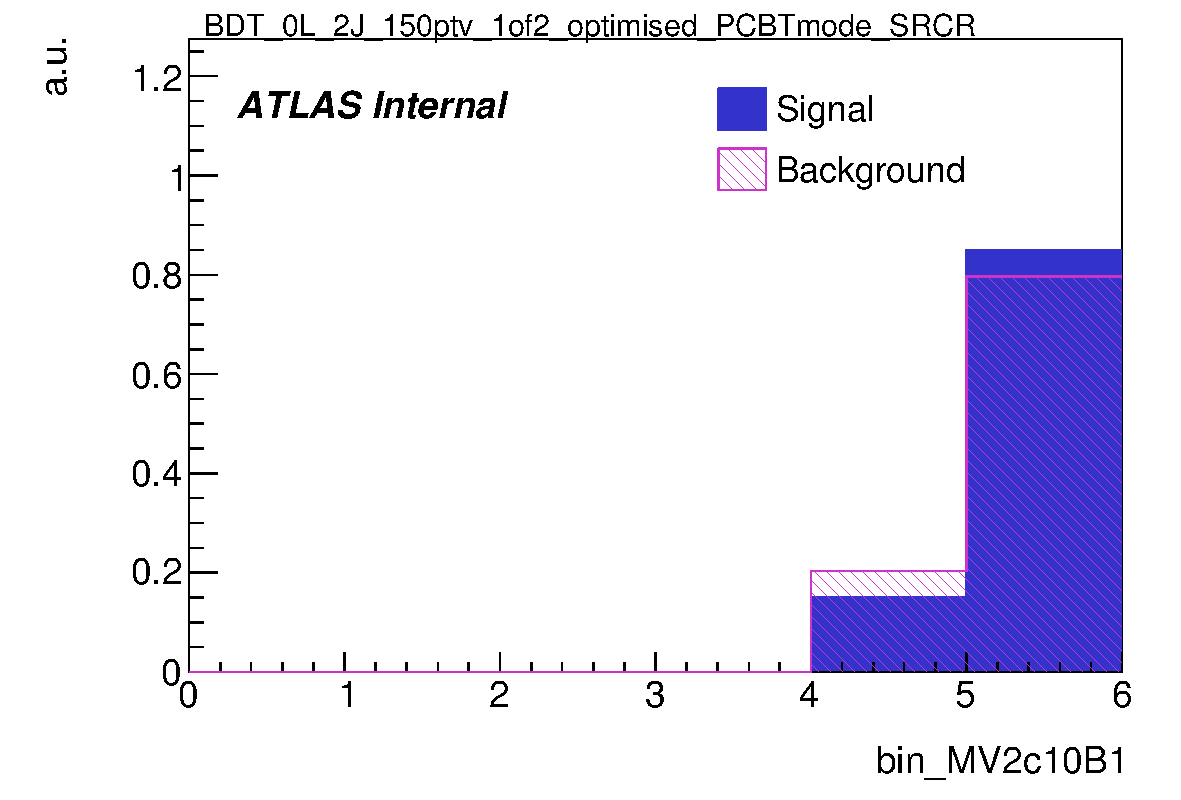
\includegraphics[width=0.33\linewidth]{0-lep-mva/Distr_SignalBackground_bin_MV2c10B1_BDT_0L_2J_150ptv_1of2_optimised_PCBTmode_SRCR-eps-converted-to}}
    \subfloat[]{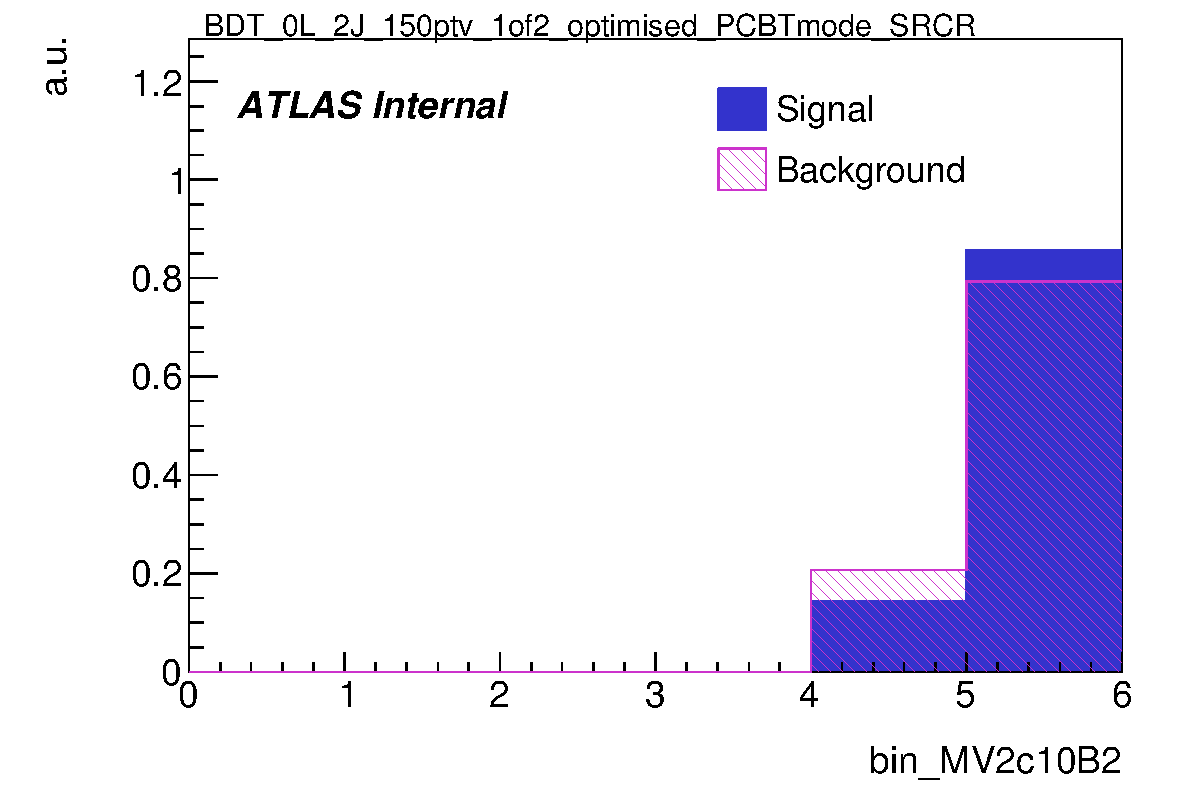
\includegraphics[width=0.33\linewidth]{0-lep-mva/Distr_SignalBackground_bin_MV2c10B2_BDT_0L_2J_150ptv_1of2_optimised_PCBTmode_SRCR-eps-converted-to}}
     \subfloat[]{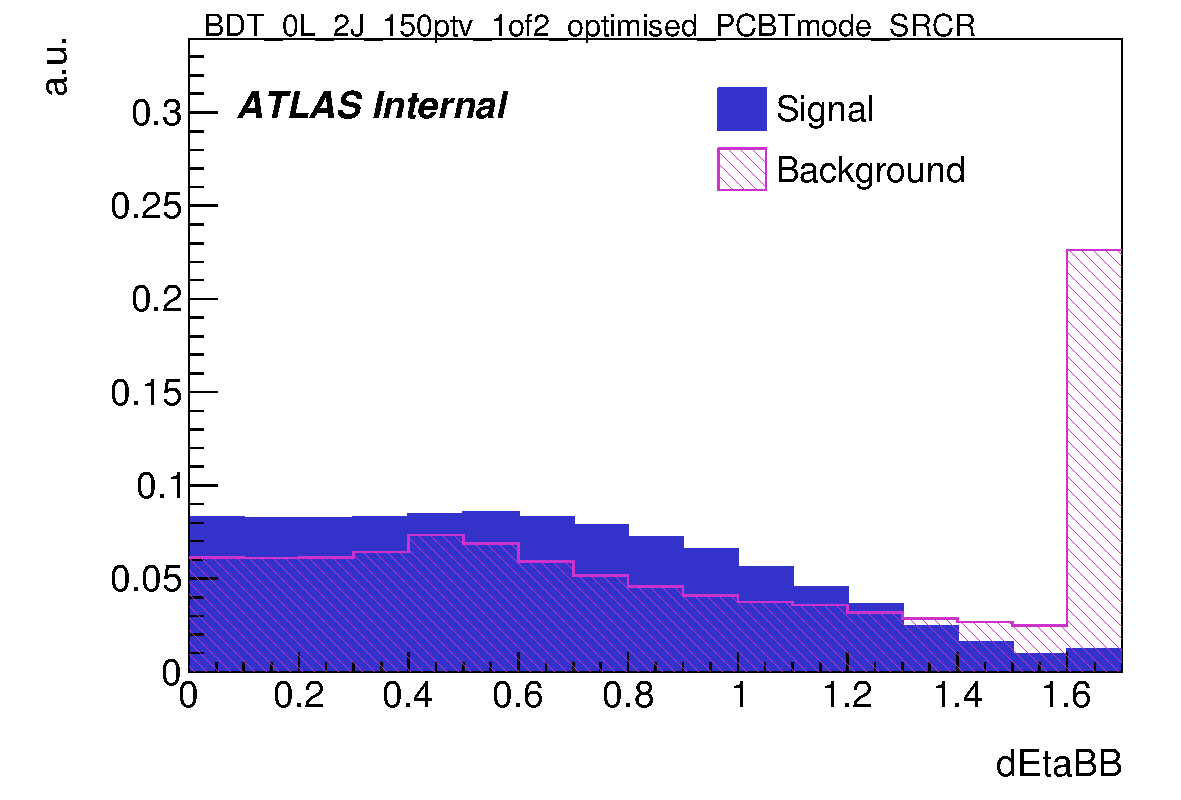
\includegraphics[width=0.33\linewidth]{0-lep-mva/Distr_SignalBackground_dEtaBB_BDT_0L_2J_150ptv_1of2_optimised_PCBTmode_SRCR-eps-converted-to}}\\
    \subfloat[]{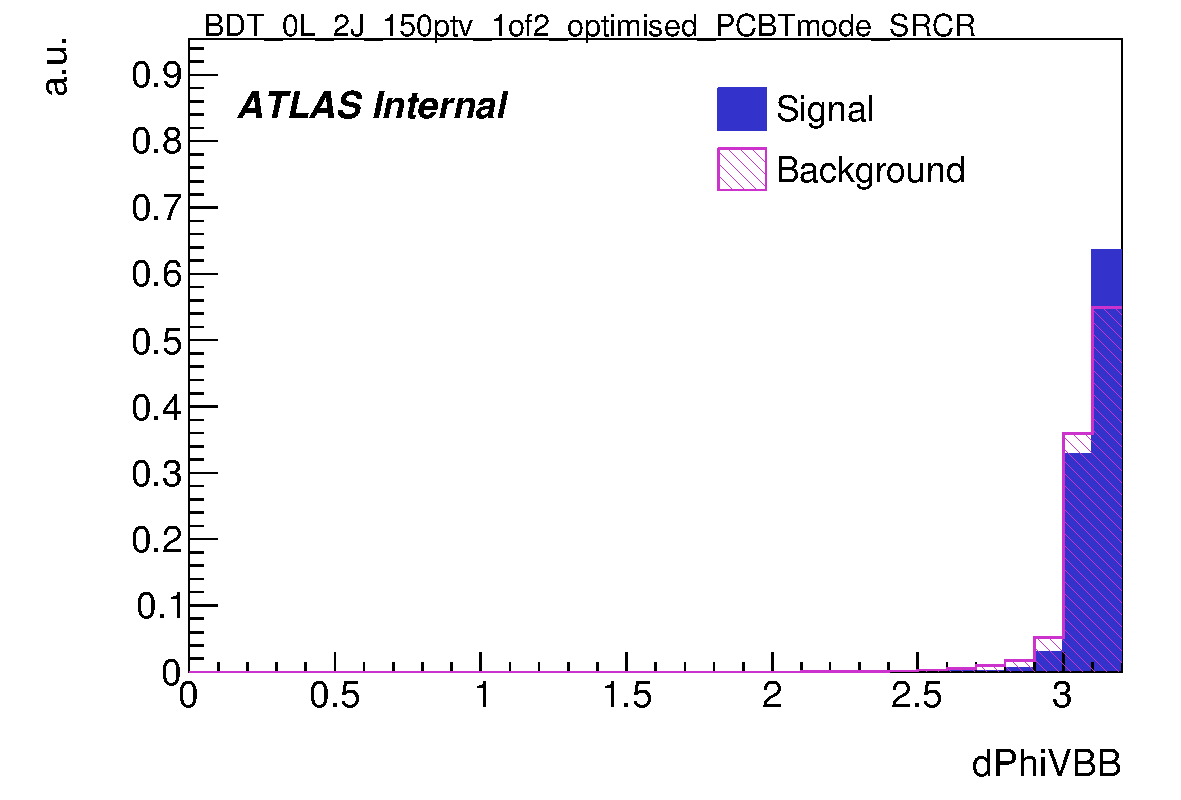
\includegraphics[width=0.33\linewidth]{0-lep-mva/Distr_SignalBackground_dPhiVBB_BDT_0L_2J_150ptv_1of2_optimised_PCBTmode_SRCR-eps-converted-to}}
    \subfloat[]{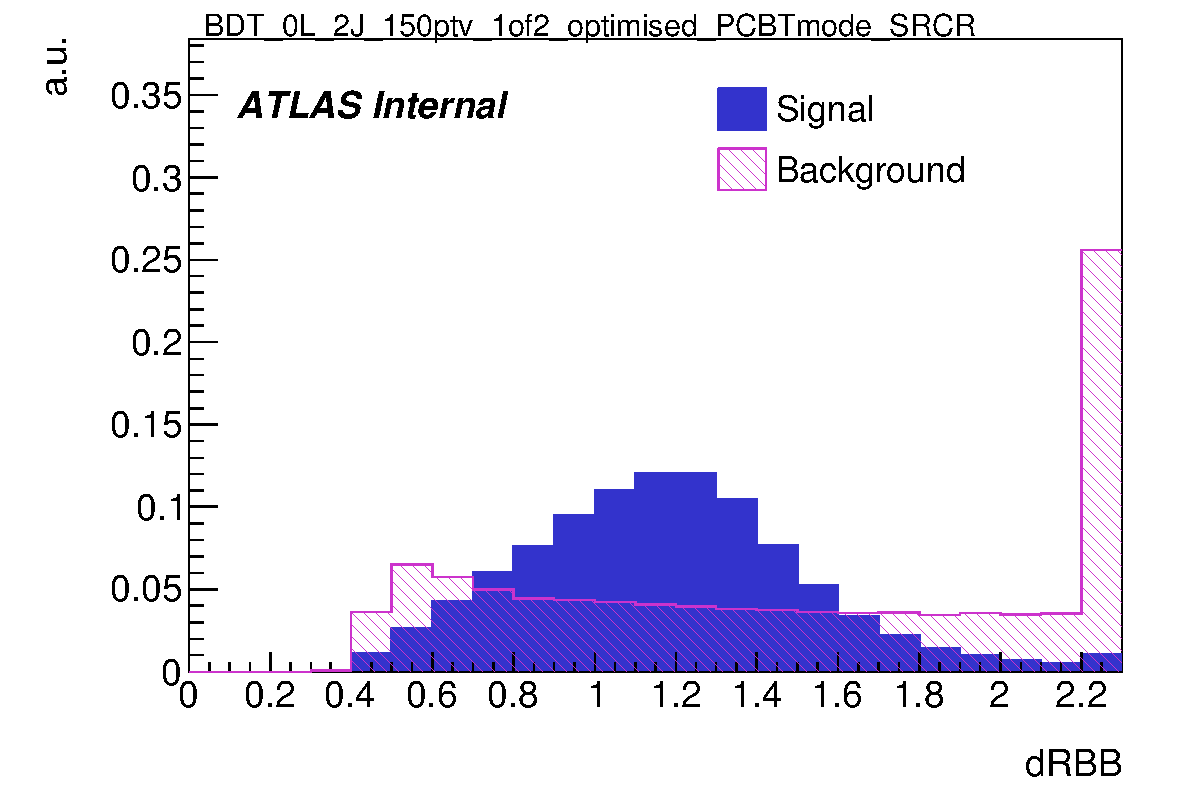
\includegraphics[width=0.33\linewidth]{0-lep-mva/Distr_SignalBackground_dRBB_BDT_0L_2J_150ptv_1of2_optimised_PCBTmode_SRCR-eps-converted-to}}
     \subfloat[]{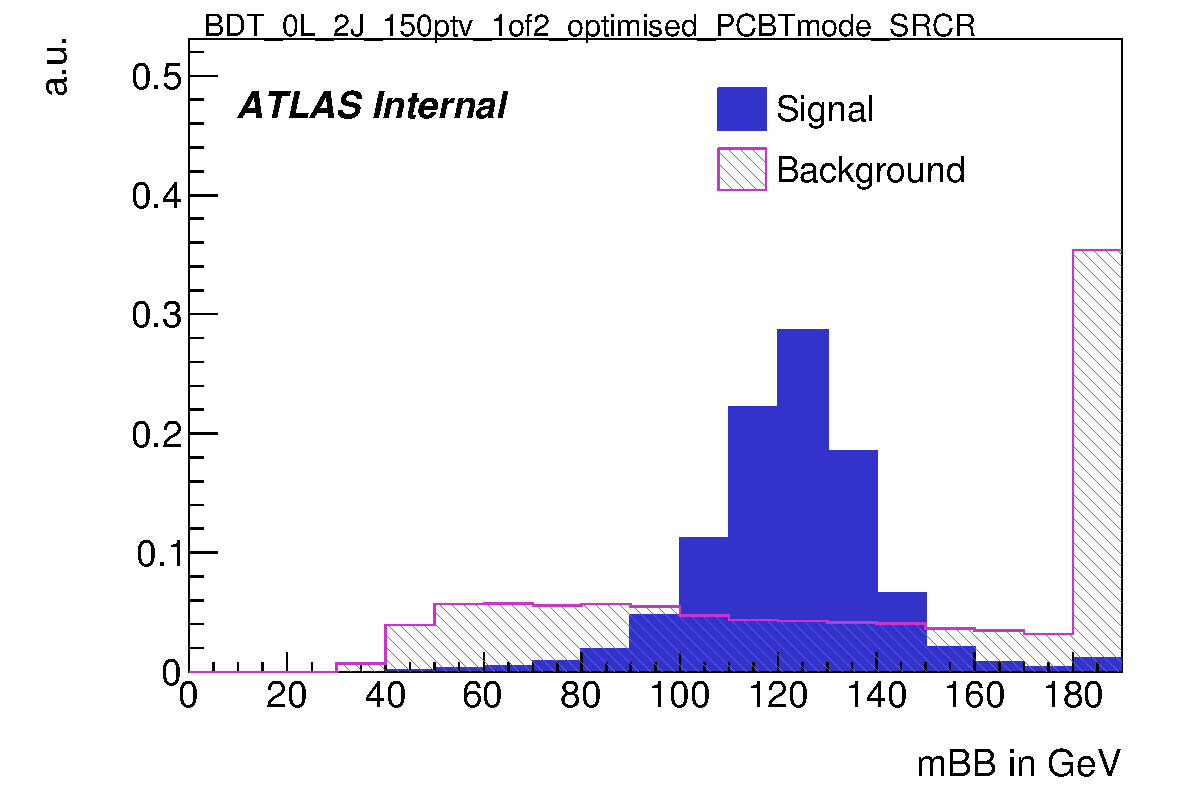
\includegraphics[width=0.33\linewidth]{0-lep-mva/Distr_SignalBackground_mBB_BDT_0L_2J_150ptv_1of2_optimised_PCBTmode_SRCR-eps-converted-to}}\\
    \subfloat[]{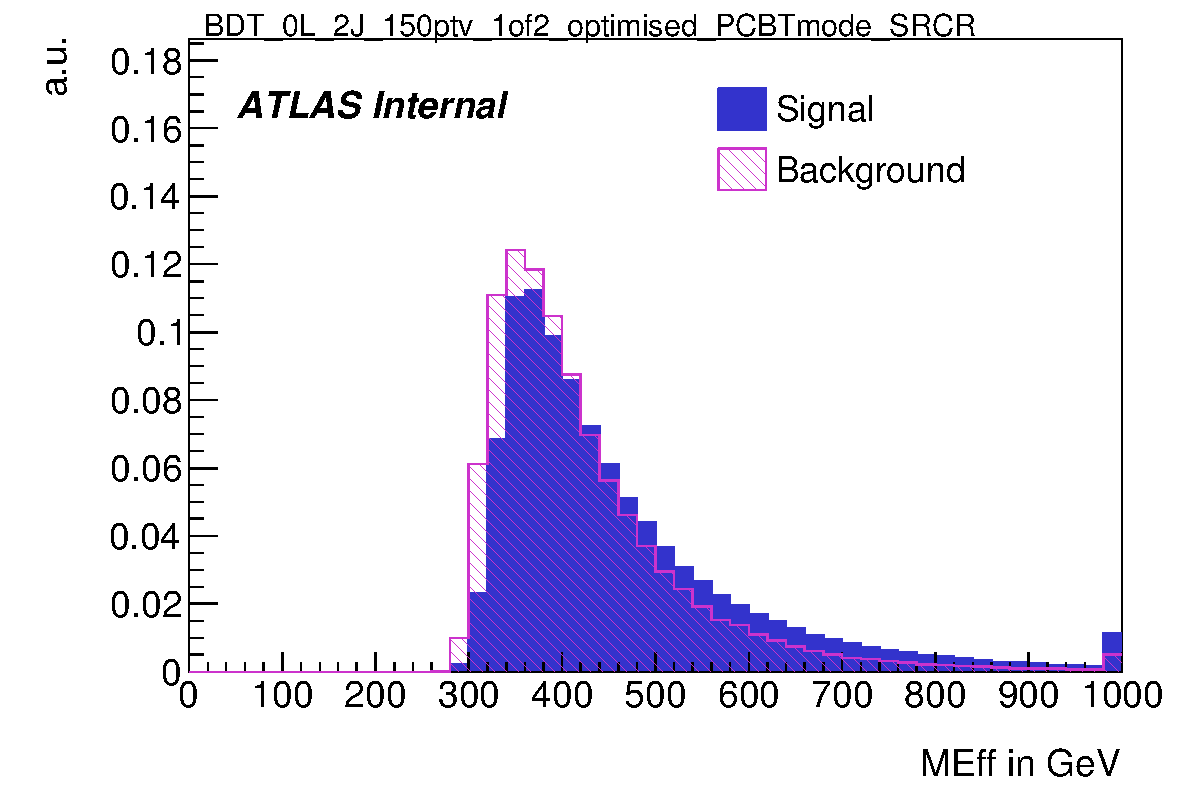
\includegraphics[width=0.33\linewidth]{0-lep-mva/Distr_SignalBackground_MEff_BDT_0L_2J_150ptv_1of2_optimised_PCBTmode_SRCR-eps-converted-to}}
     \subfloat[]{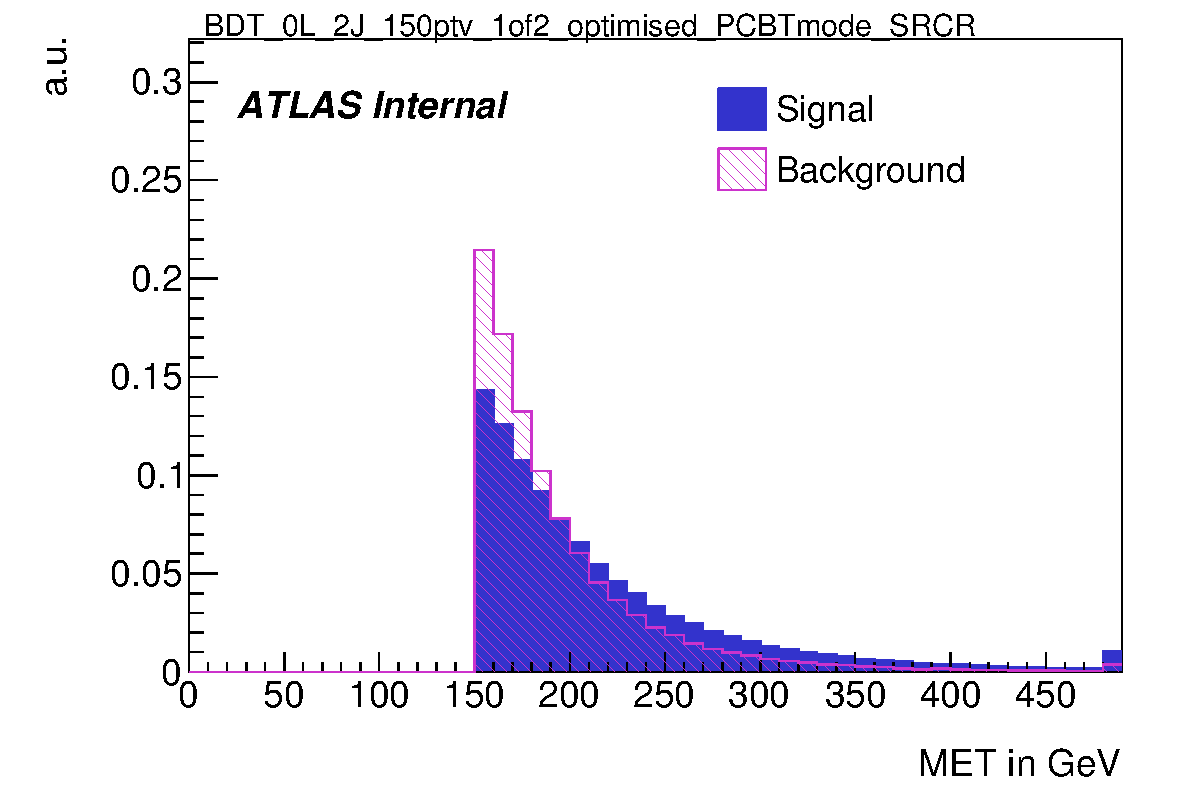
\includegraphics[width=0.33\linewidth]{0-lep-mva/Distr_SignalBackground_MET_BDT_0L_2J_150ptv_1of2_optimised_PCBTmode_SRCR-eps-converted-to}}          
    \subfloat[]{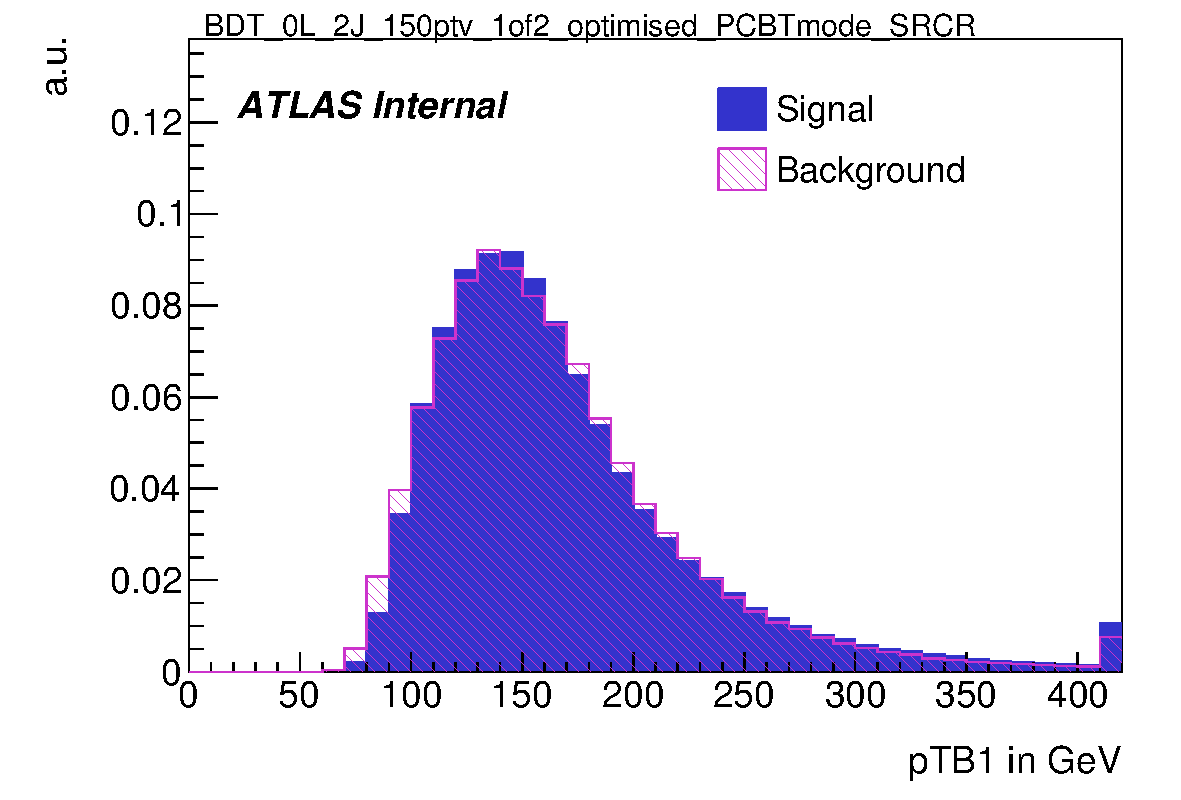
\includegraphics[width=0.33\linewidth]{0-lep-mva/Distr_SignalBackground_pTB1_BDT_0L_2J_150ptv_1of2_optimised_PCBTmode_SRCR-eps-converted-to}} \\
    \subfloat[]{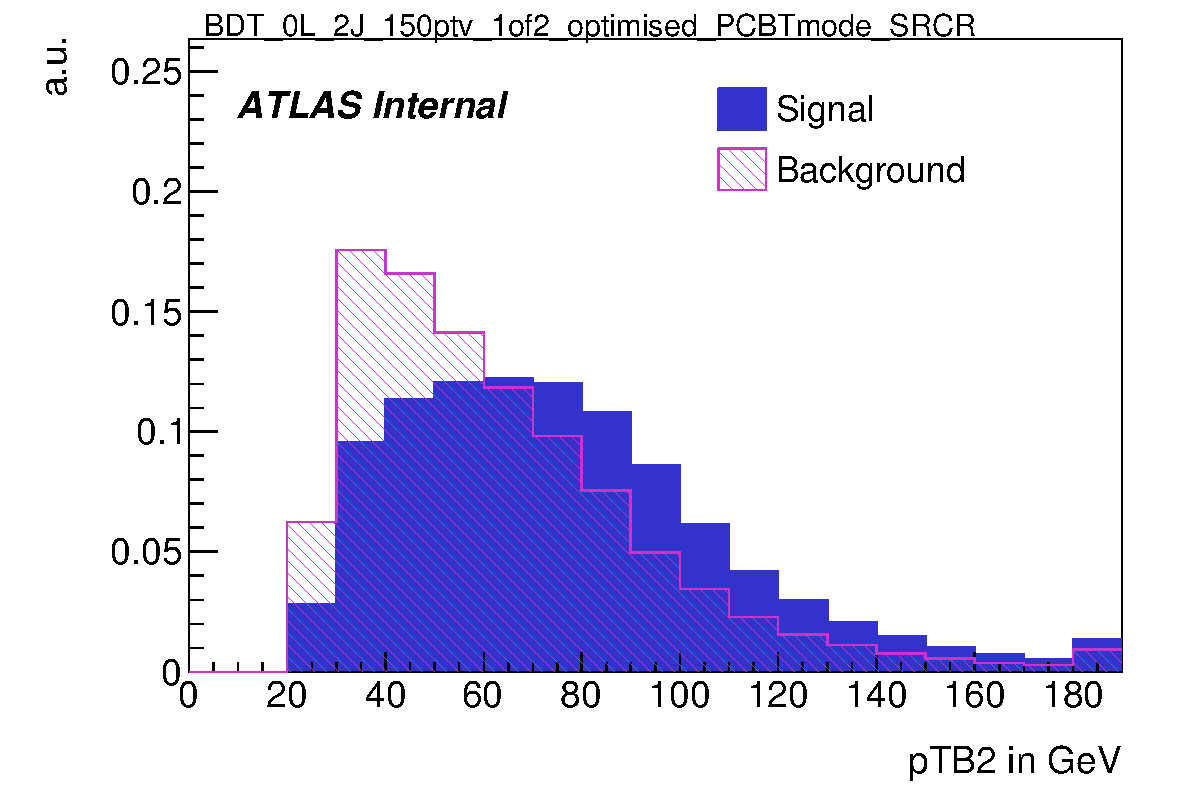
\includegraphics[width=0.33\linewidth]{0-lep-mva/Distr_SignalBackground_pTB2_BDT_0L_2J_150ptv_1of2_optimised_PCBTmode_SRCR-eps-converted-to}}   
    \subfloat[]{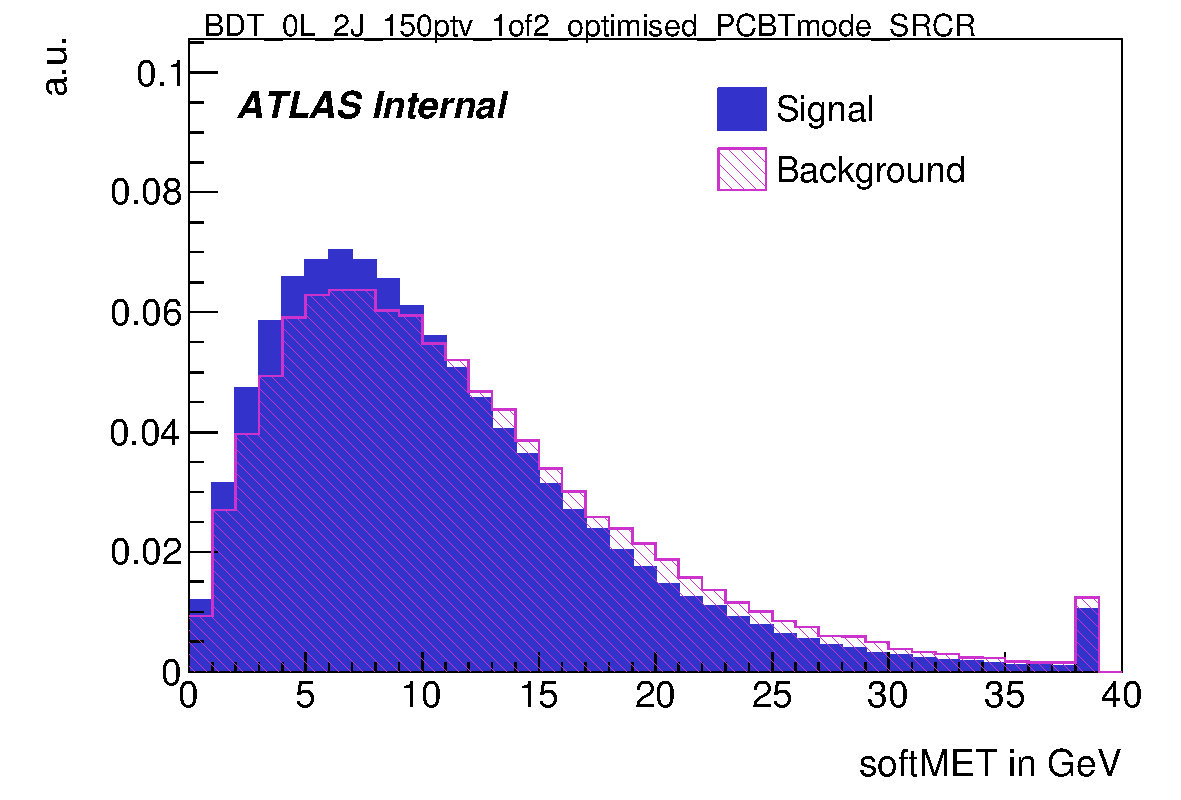
\includegraphics[width=0.33\linewidth]{0-lep-mva/Distr_SignalBackground_softMET_BDT_0L_2J_150ptv_1of2_optimised_PCBTmode_SRCR-eps-converted-to}}\\    
    \end{tabular}
    \caption[Inputs to the multi-variate analysis in the 0--lepton 2--jet
    region.]{Inputs to the multi-variate analysis in the 0--lepton 2--jet
      region. Signal events are shown in blue and background events are shown in
      red. The signal and background histograms have been normalised to the same
      area. The distributions only include events with $E_T^{\text{miss}}$ > 150
      \GeV.}
    \label{fig:bdtinputs-0lep}
\end{figure}

 \begin{figure}[htbp]
  \centering
  \begin{tabular}{cccc}
    \subfloat[]{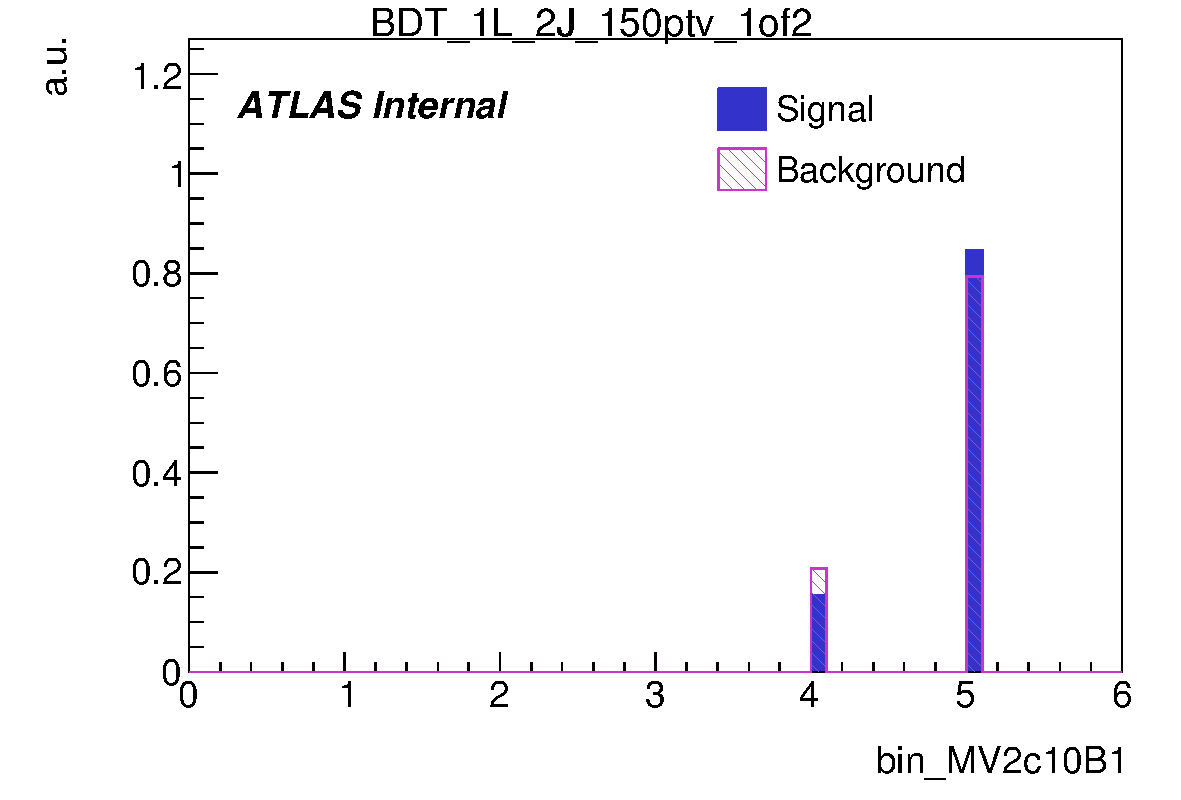
\includegraphics[width=0.3\linewidth]{1-lep-mva/Distr_SignalBackground_bin_MV2c10B1_BDT_1L_2J_150ptv_1of2-eps-converted-to}}
    \subfloat[]{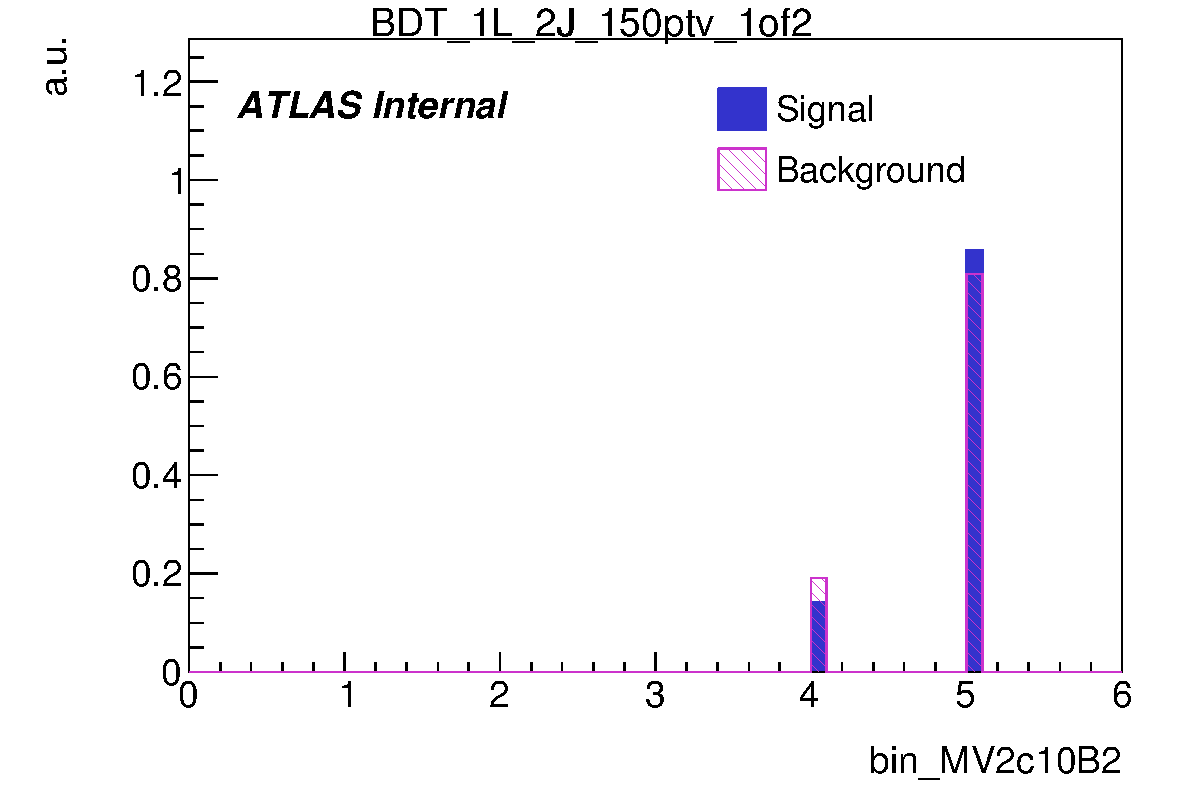
\includegraphics[width=0.3\linewidth]{1-lep-mva/Distr_SignalBackground_bin_MV2c10B2_BDT_1L_2J_150ptv_1of2-eps-converted-to}}
     \subfloat[]{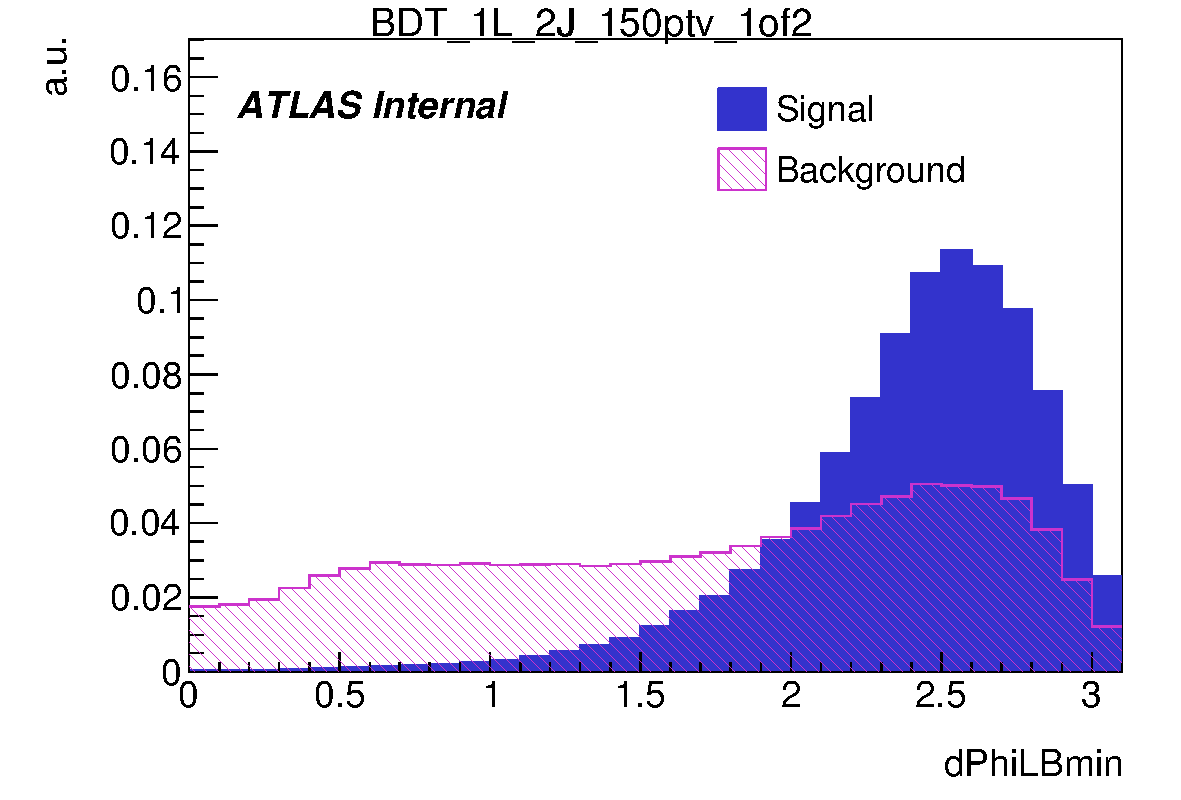
\includegraphics[width=0.3\linewidth]{1-lep-mva/Distr_SignalBackground_dPhiLBmin_BDT_1L_2J_150ptv_1of2-eps-converted-to}}\\
    \subfloat[]{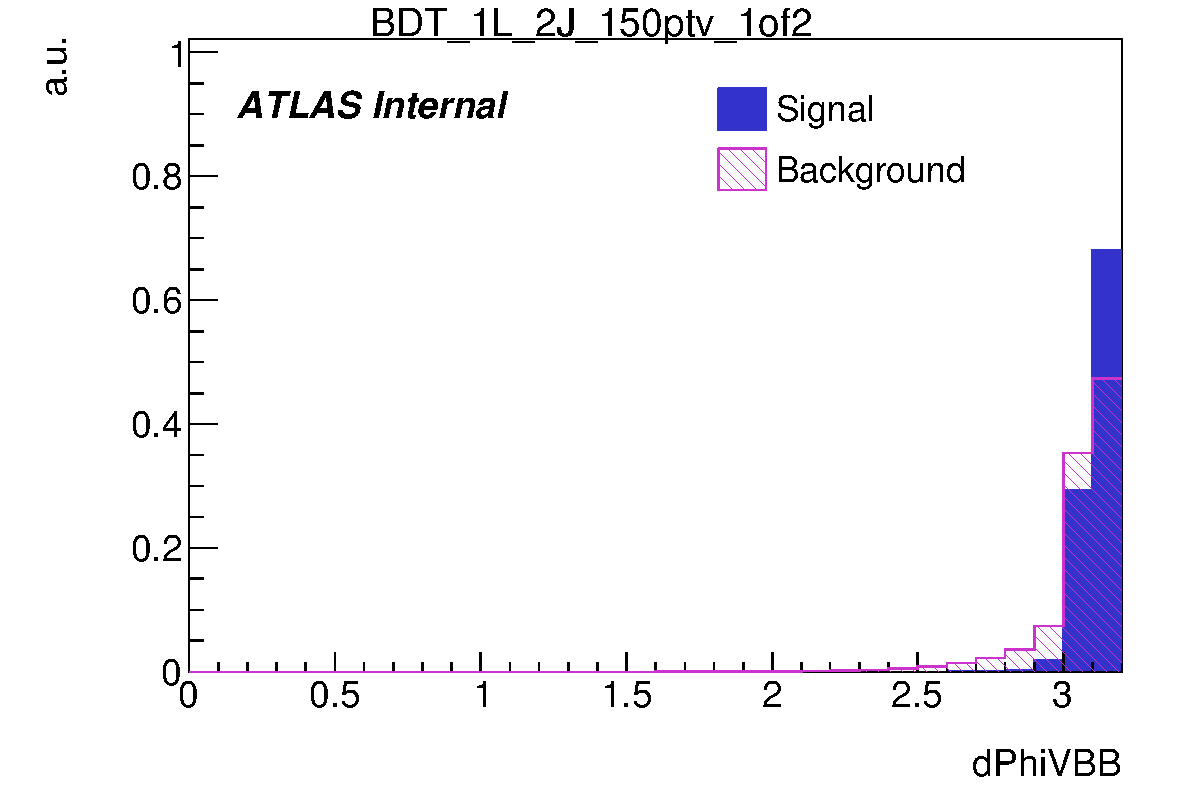
\includegraphics[width=0.3\linewidth]{1-lep-mva/Distr_SignalBackground_dPhiVBB_BDT_1L_2J_150ptv_1of2-eps-converted-to}}
    \subfloat[]{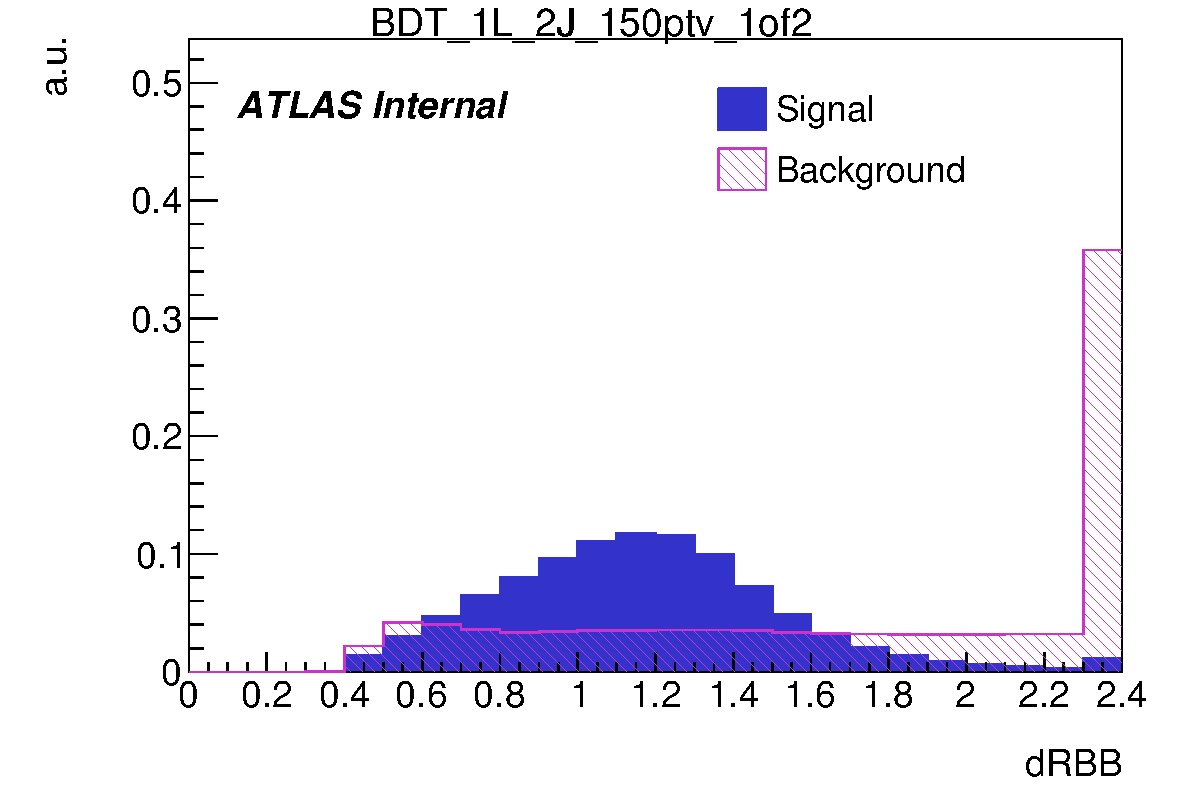
\includegraphics[width=0.3\linewidth]{1-lep-mva/Distr_SignalBackground_dRBB_BDT_1L_2J_150ptv_1of2-eps-converted-to}}
     \subfloat[]{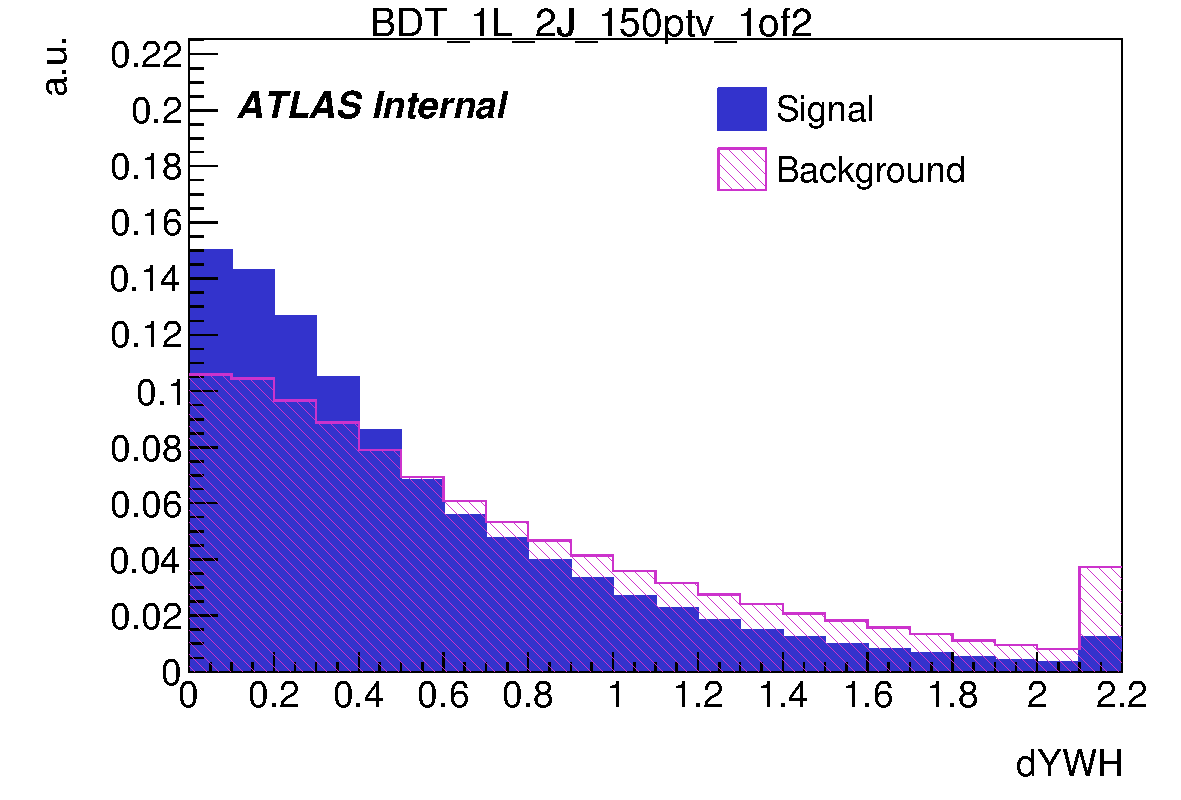
\includegraphics[width=0.3\linewidth]{1-lep-mva/Distr_SignalBackground_dYWH_BDT_1L_2J_150ptv_1of2-eps-converted-to}}\\
    \subfloat[]{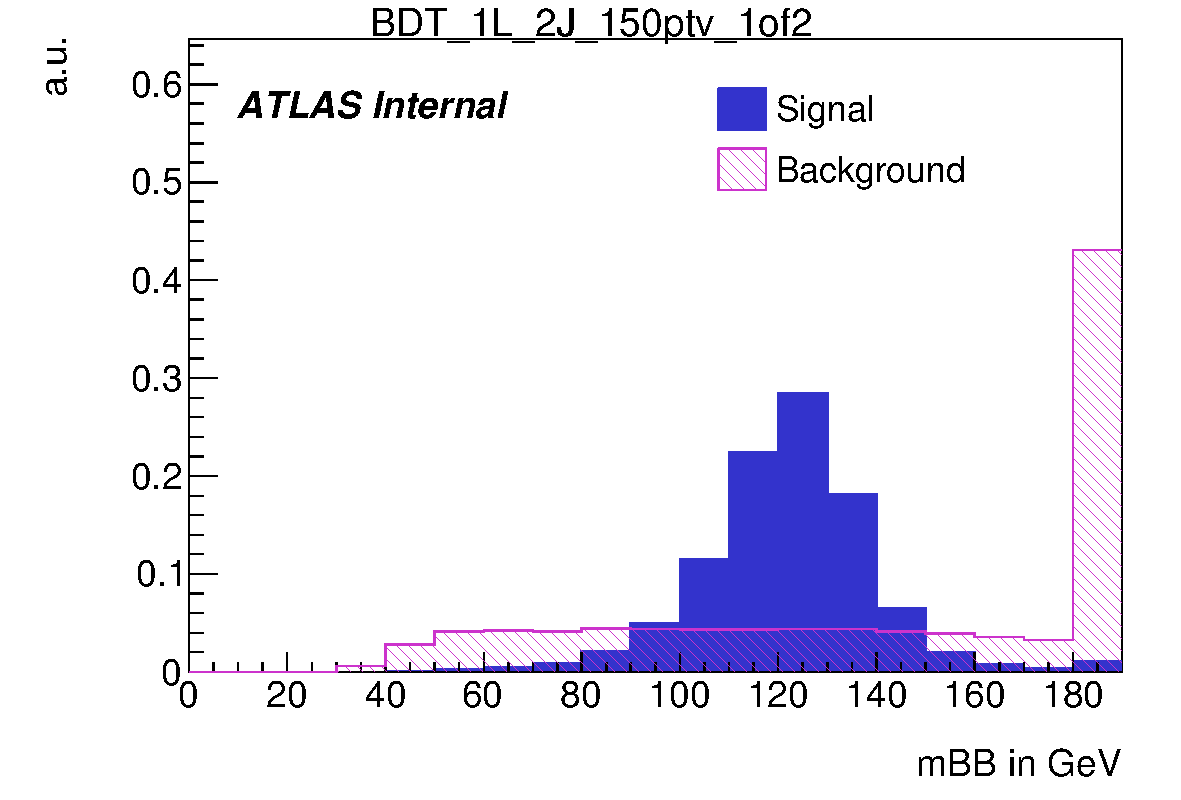
\includegraphics[width=0.3\linewidth]{1-lep-mva/Distr_SignalBackground_mBB_BDT_1L_2J_150ptv_1of2-eps-converted-to}}
     \subfloat[]{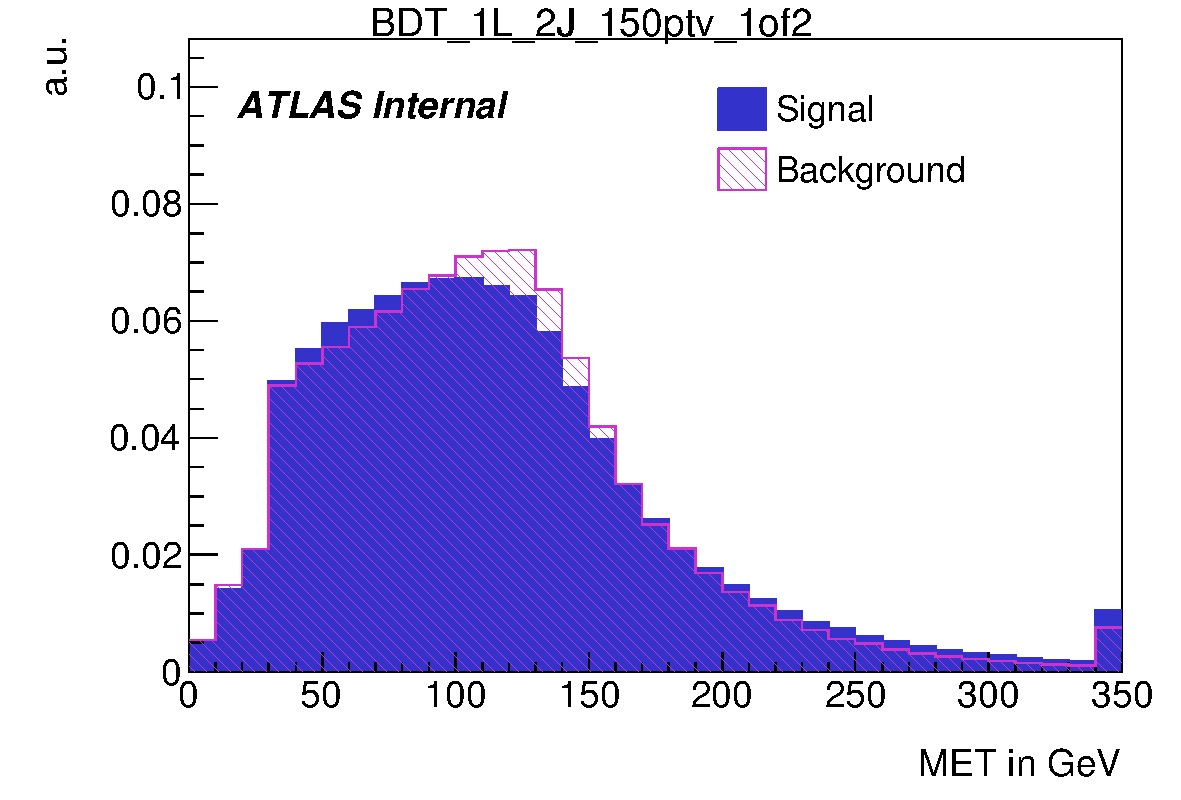
\includegraphics[width=0.3\linewidth]{1-lep-mva/Distr_SignalBackground_MET_BDT_1L_2J_150ptv_1of2-eps-converted-to}}          
    \subfloat[]{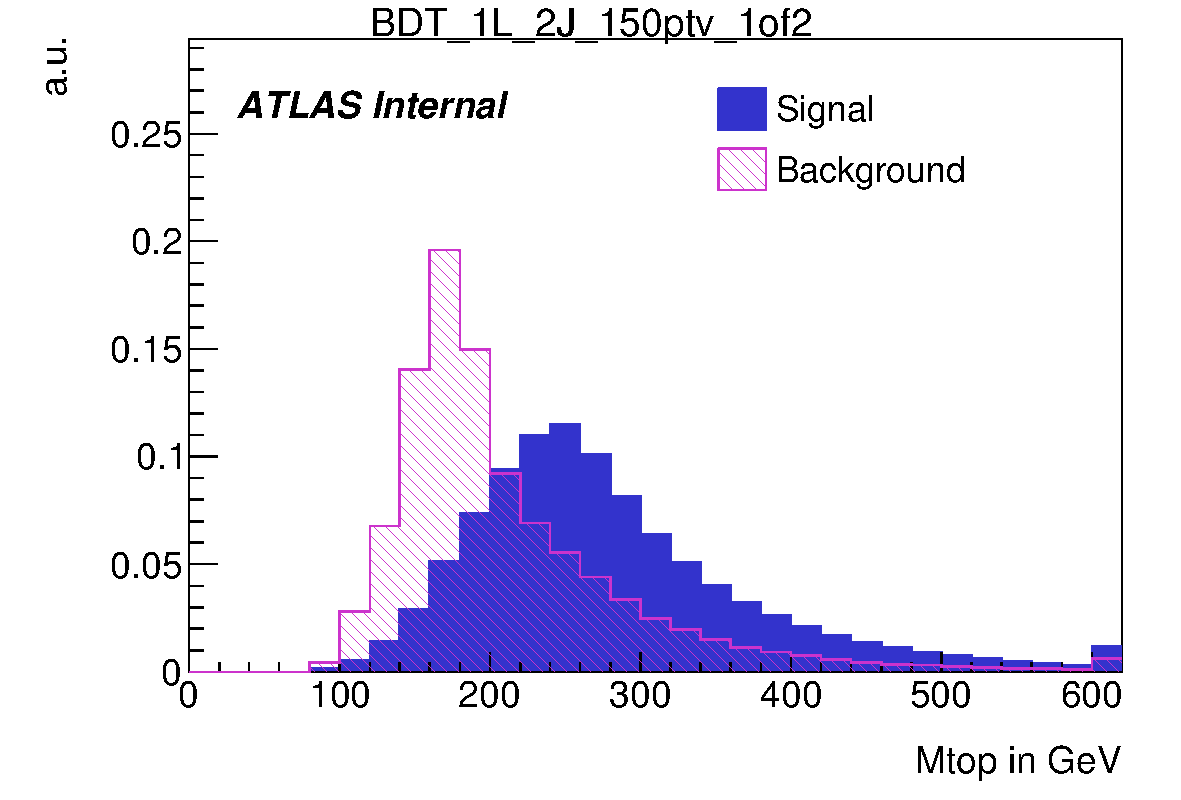
\includegraphics[width=0.3\linewidth]{1-lep-mva/Distr_SignalBackground_Mtop_BDT_1L_2J_150ptv_1of2-eps-converted-to}} \\
    \subfloat[]{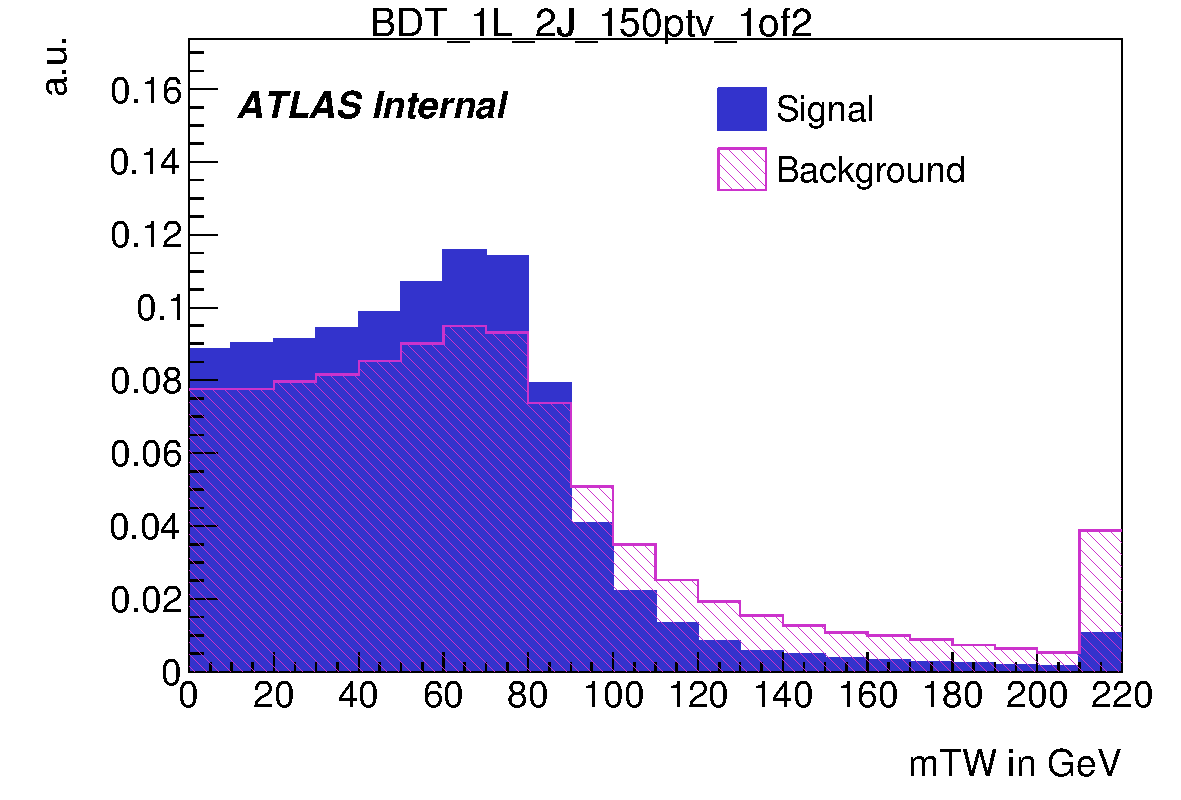
\includegraphics[width=0.3\linewidth]{1-lep-mva/Distr_SignalBackground_mTW_BDT_1L_2J_150ptv_1of2-eps-converted-to}}   
    \subfloat[]{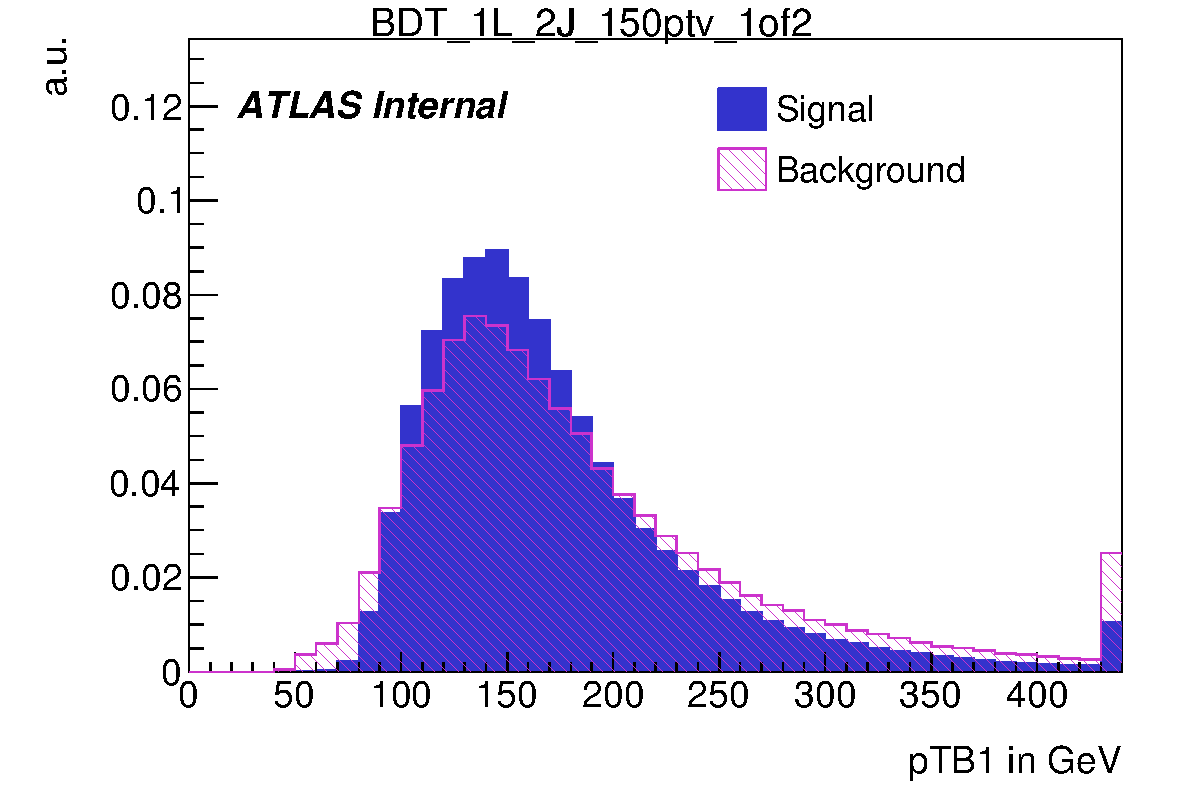
\includegraphics[width=0.3\linewidth]{1-lep-mva/Distr_SignalBackground_pTB1_BDT_1L_2J_150ptv_1of2-eps-converted-to}}
    \subfloat[]{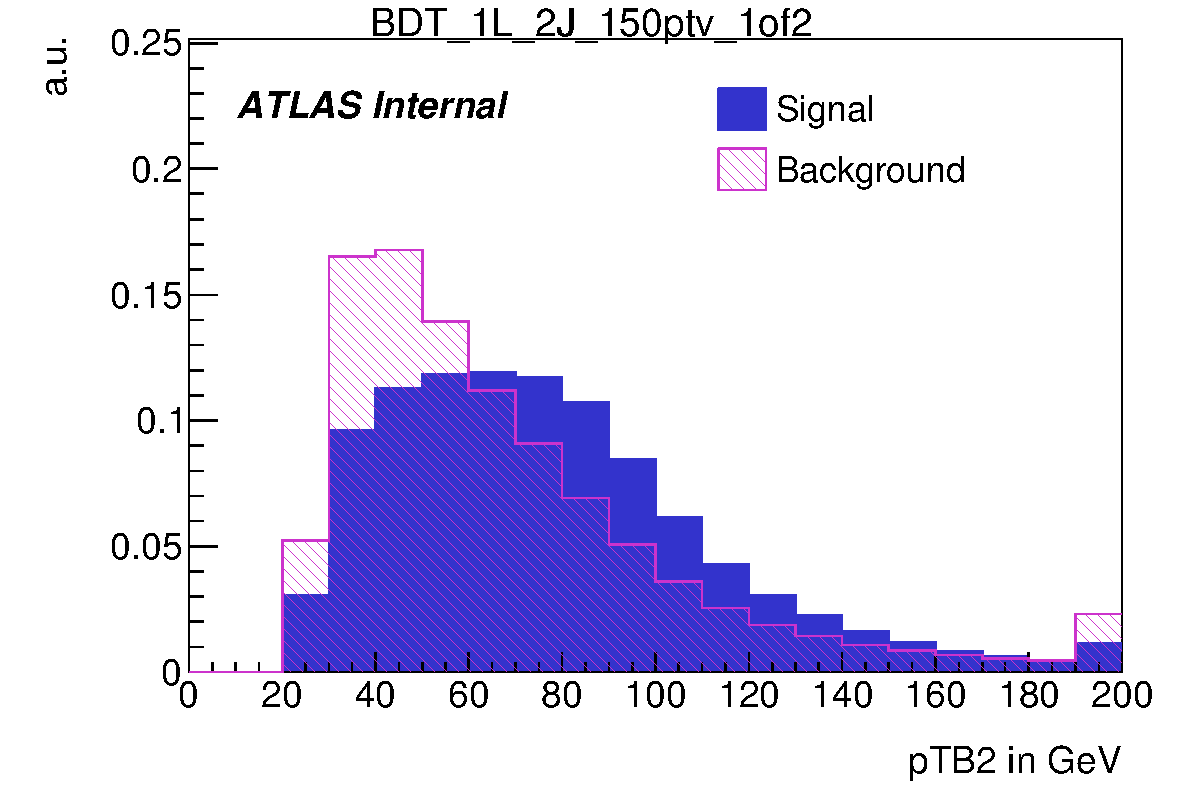
\includegraphics[width=0.3\linewidth]{1-lep-mva/Distr_SignalBackground_pTB2_BDT_1L_2J_150ptv_1of2-eps-converted-to}}\\   
    \subfloat[]{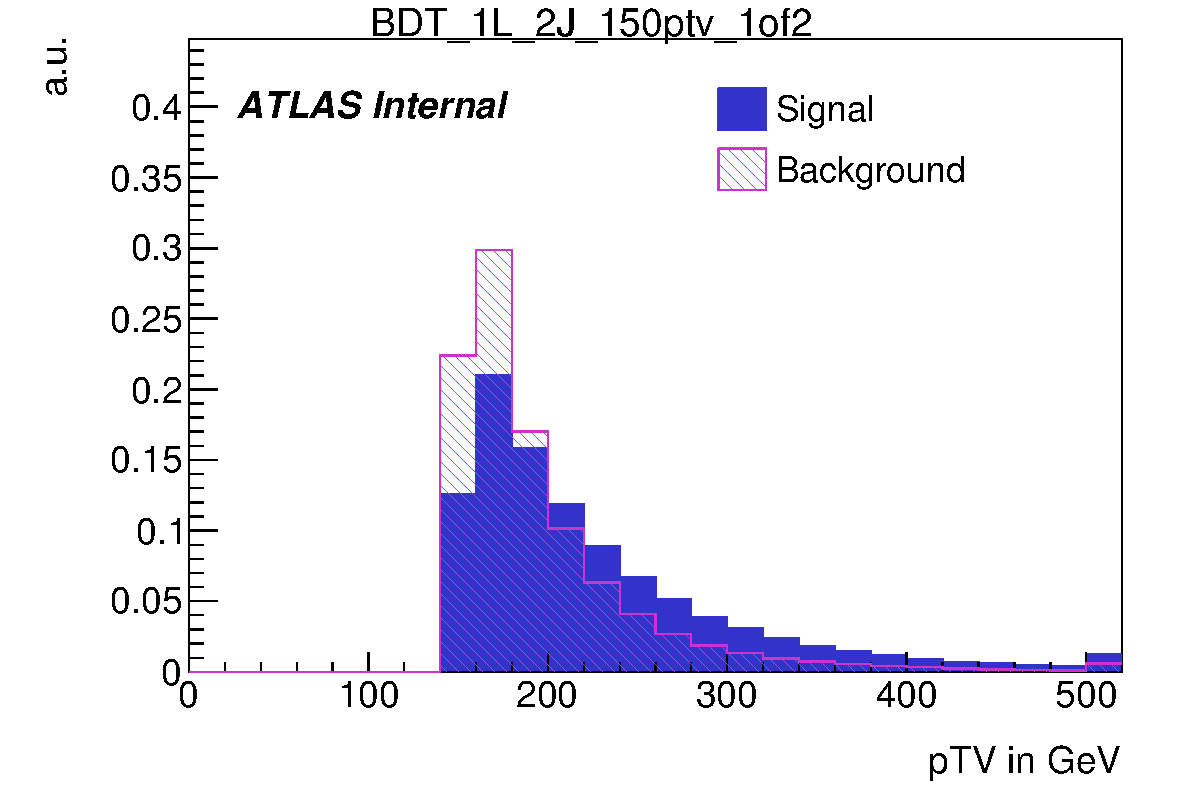
\includegraphics[width=0.3\linewidth]{1-lep-mva/Distr_SignalBackground_pTV_BDT_1L_2J_150ptv_1of2-eps-converted-to}} 
    \end{tabular}
    \caption[Inputs to the multi-variate analysis in the 1--lepton 2--jet
    region.]{Inputs to the multi-variate analysis in the 1--lepton 2--jet
      region. Signal events are shown in blue and background events are shown in
      red. The signal and background histograms have been normalised to the same
      area.The distributions only include events with $p_T^{W}$ > 150
      \GeV.}
    \label{fig:bdtinputs-1lep}
\end{figure}

 \begin{figure}[htbp]
  \centering
  \begin{tabular}{cccc}
    \subfloat[]{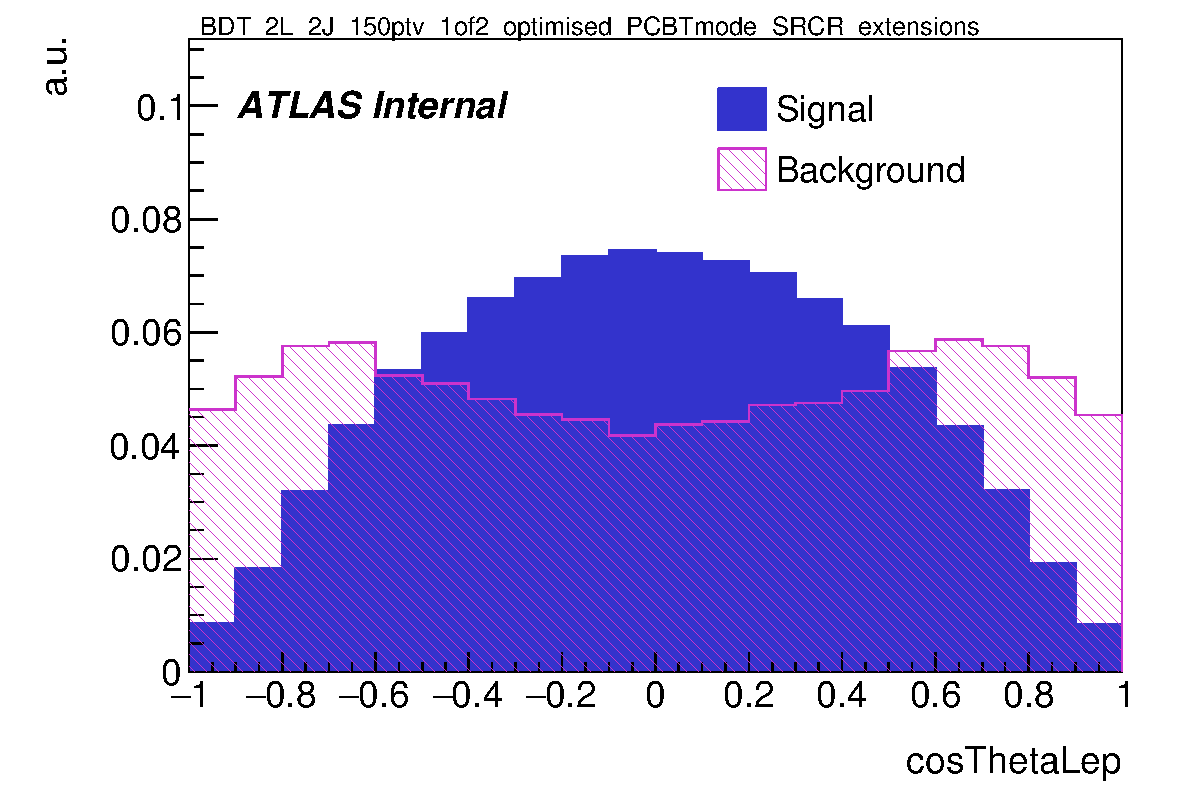
\includegraphics[width=0.33\linewidth]{2-lep-mva/Distr_SignalBackground_cosThetaLep_BDT_2L_2J_150ptv_1of2_optimised_PCBTmode_SRCR_extensions-eps-converted-to}}
    \subfloat[]{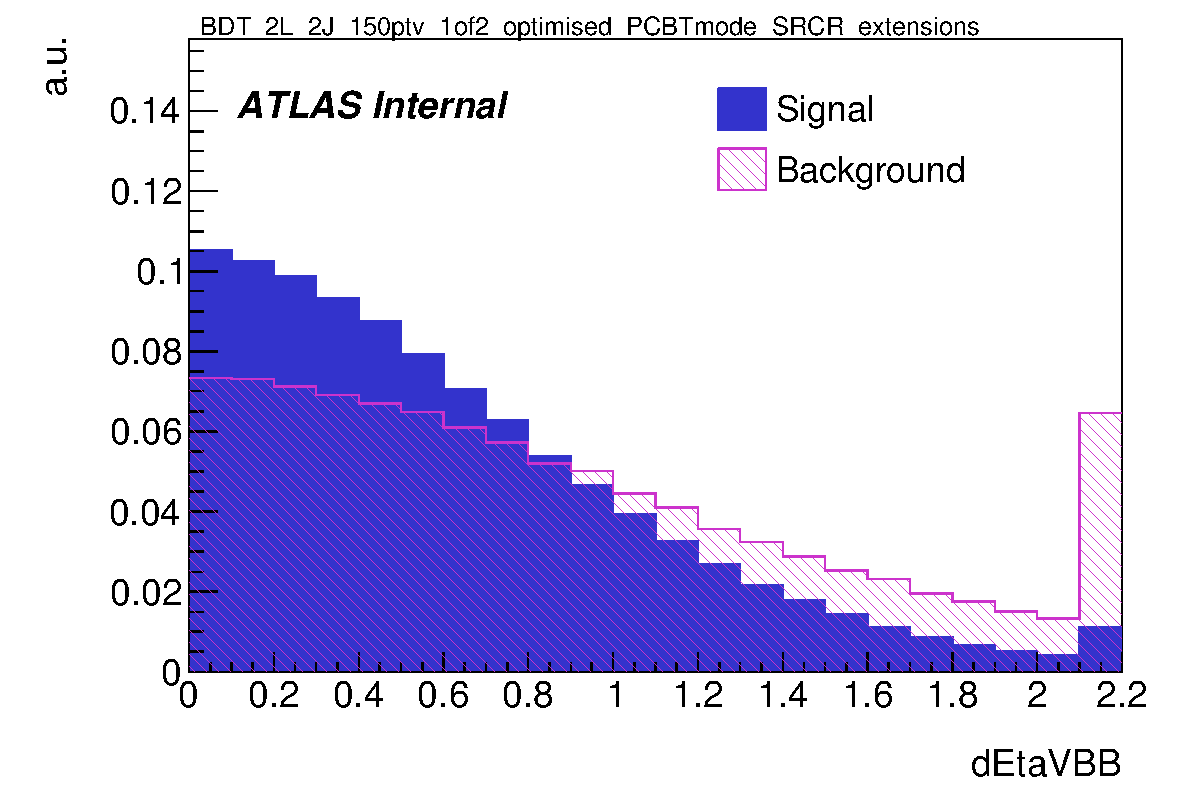
\includegraphics[width=0.33\linewidth]{2-lep-mva/Distr_SignalBackground_dEtaVBB_BDT_2L_2J_150ptv_1of2_optimised_PCBTmode_SRCR_extensions-eps-converted-to}}
     \subfloat[]{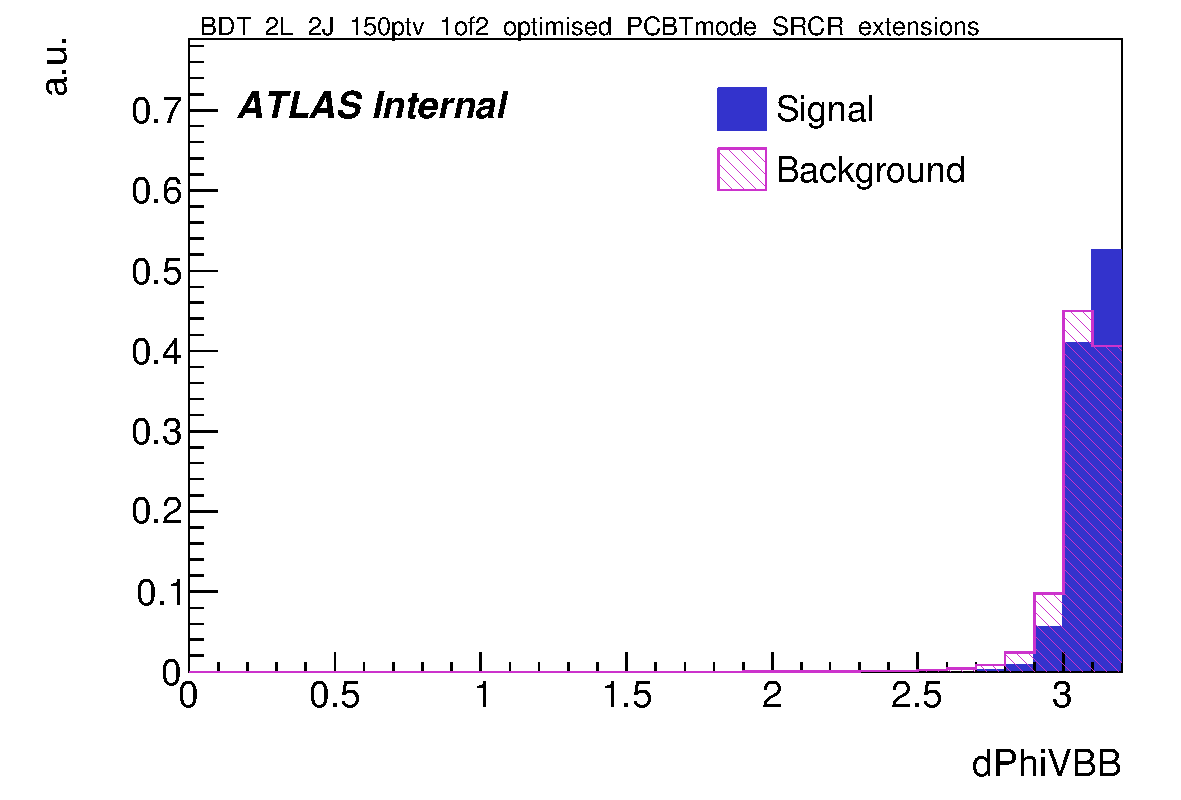
\includegraphics[width=0.33\linewidth]{2-lep-mva/Distr_SignalBackground_dPhiVBB_BDT_2L_2J_150ptv_1of2_optimised_PCBTmode_SRCR_extensions-eps-converted-to}}\\
    \subfloat[]{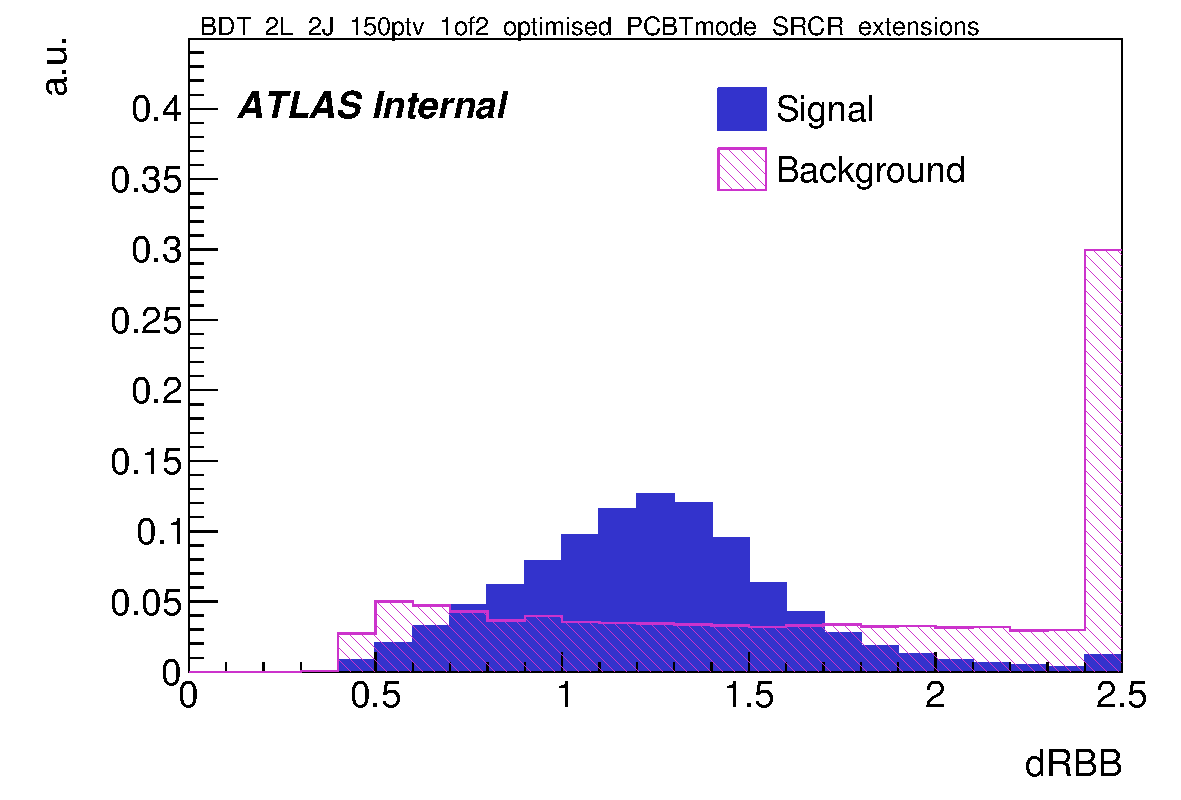
\includegraphics[width=0.33\linewidth]{2-lep-mva/Distr_SignalBackground_dRBB_BDT_2L_2J_150ptv_1of2_optimised_PCBTmode_SRCR_extensions-eps-converted-to}}
    \subfloat[]{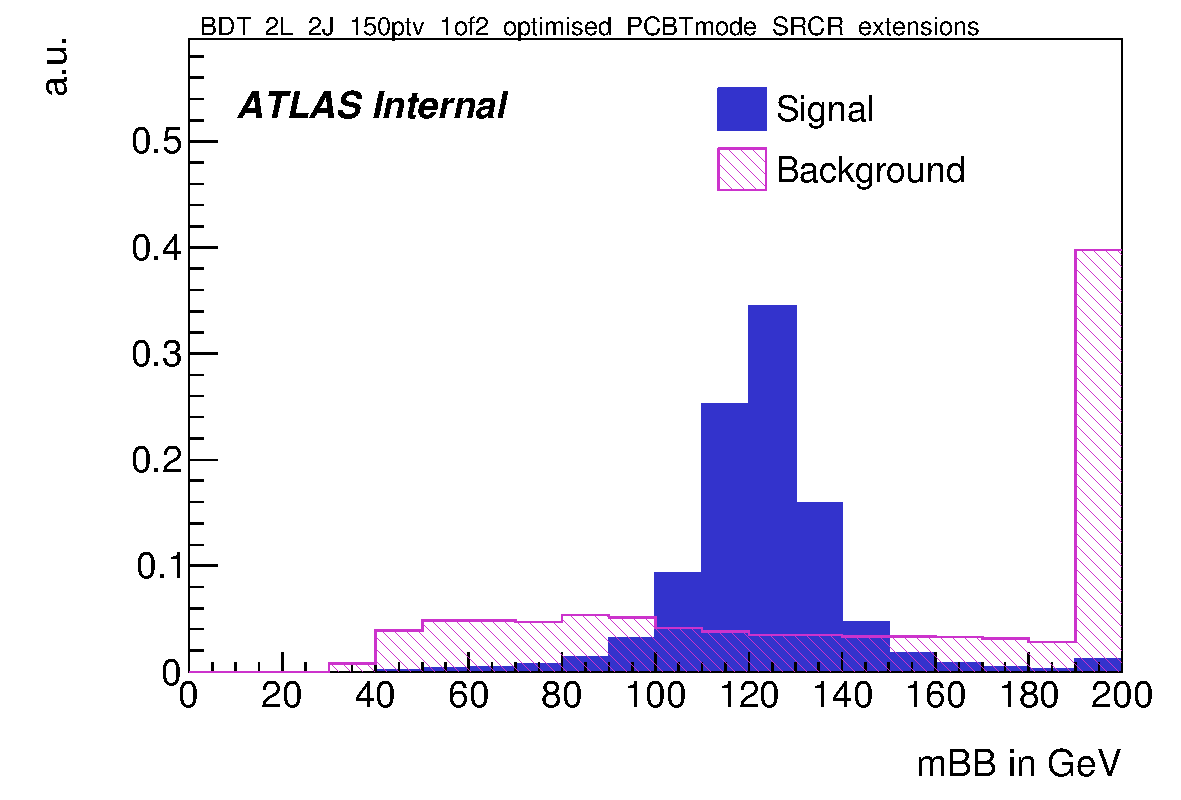
\includegraphics[width=0.33\linewidth]{2-lep-mva/Distr_SignalBackground_mBB_BDT_2L_2J_150ptv_1of2_optimised_PCBTmode_SRCR_extensions-eps-converted-to}}
     \subfloat[]{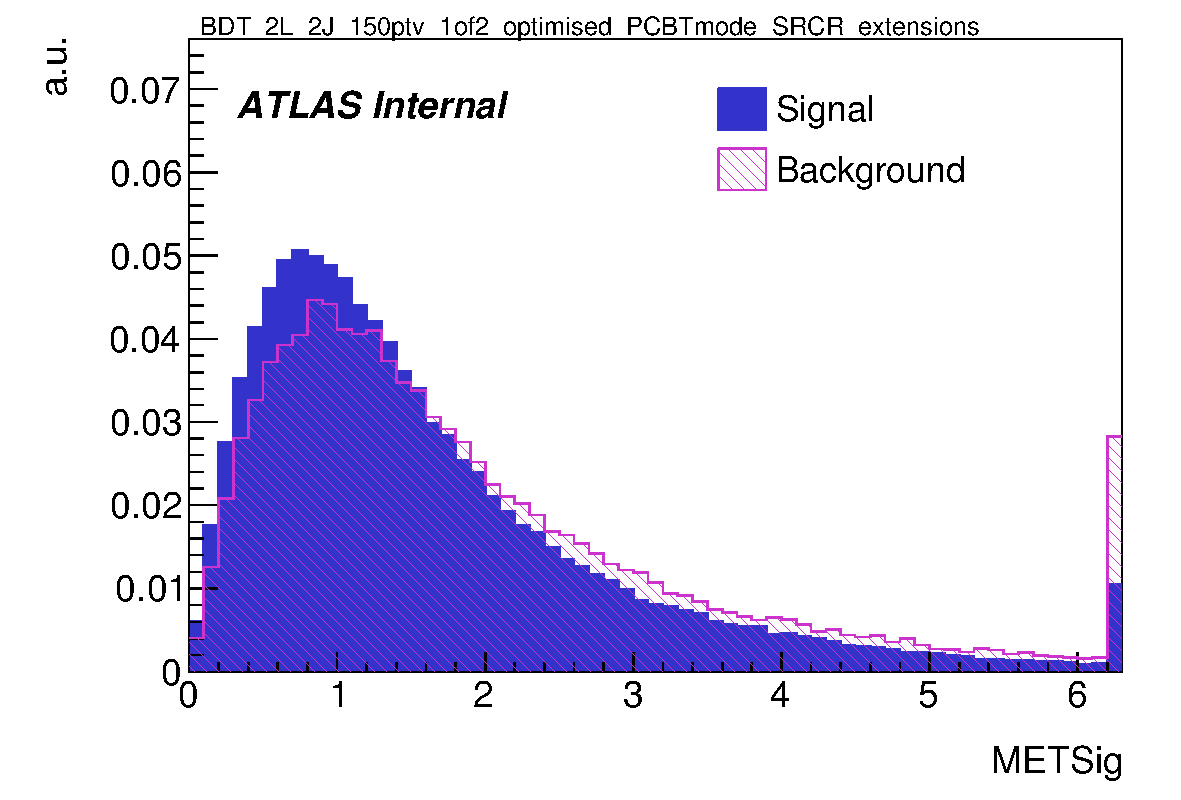
\includegraphics[width=0.33\linewidth]{2-lep-mva/Distr_SignalBackground_METSig_BDT_2L_2J_150ptv_1of2_optimised_PCBTmode_SRCR_extensions-eps-converted-to}}\\
    \subfloat[]{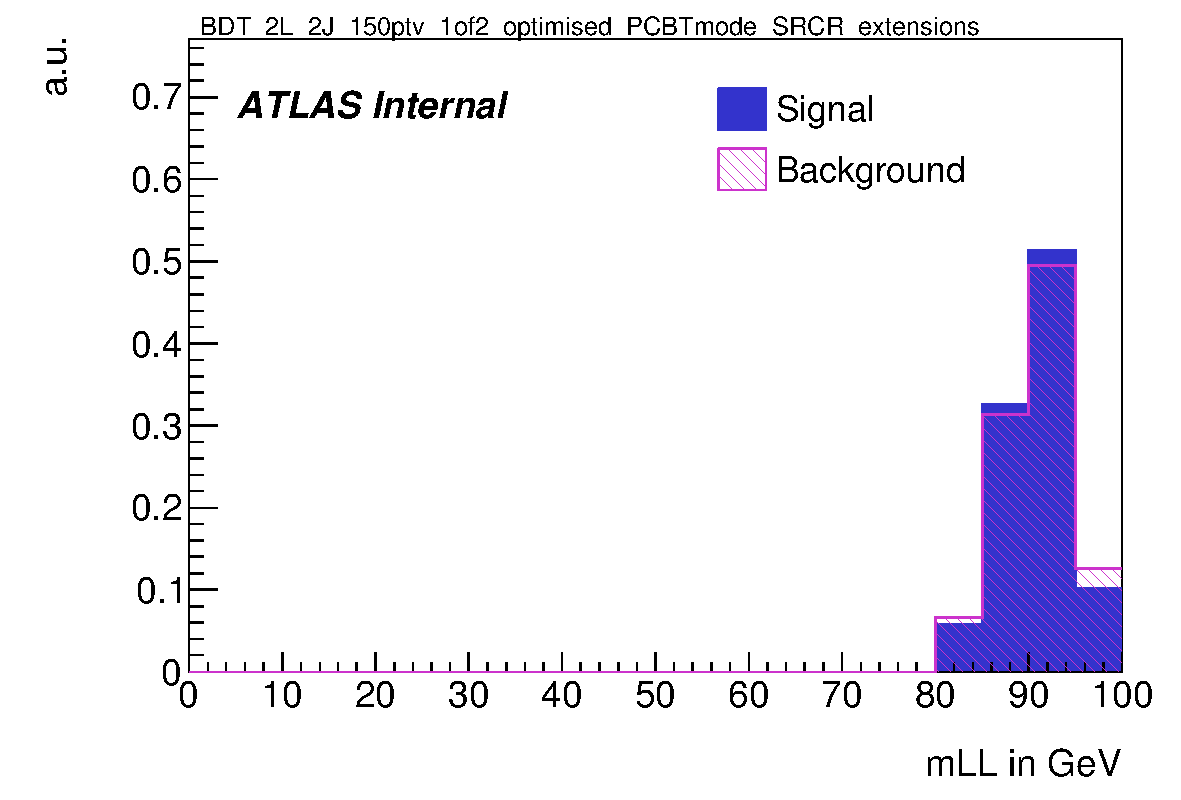
\includegraphics[width=0.33\linewidth]{2-lep-mva/Distr_SignalBackground_mLL_BDT_2L_2J_150ptv_1of2_optimised_PCBTmode_SRCR_extensions-eps-converted-to}}
     \subfloat[]{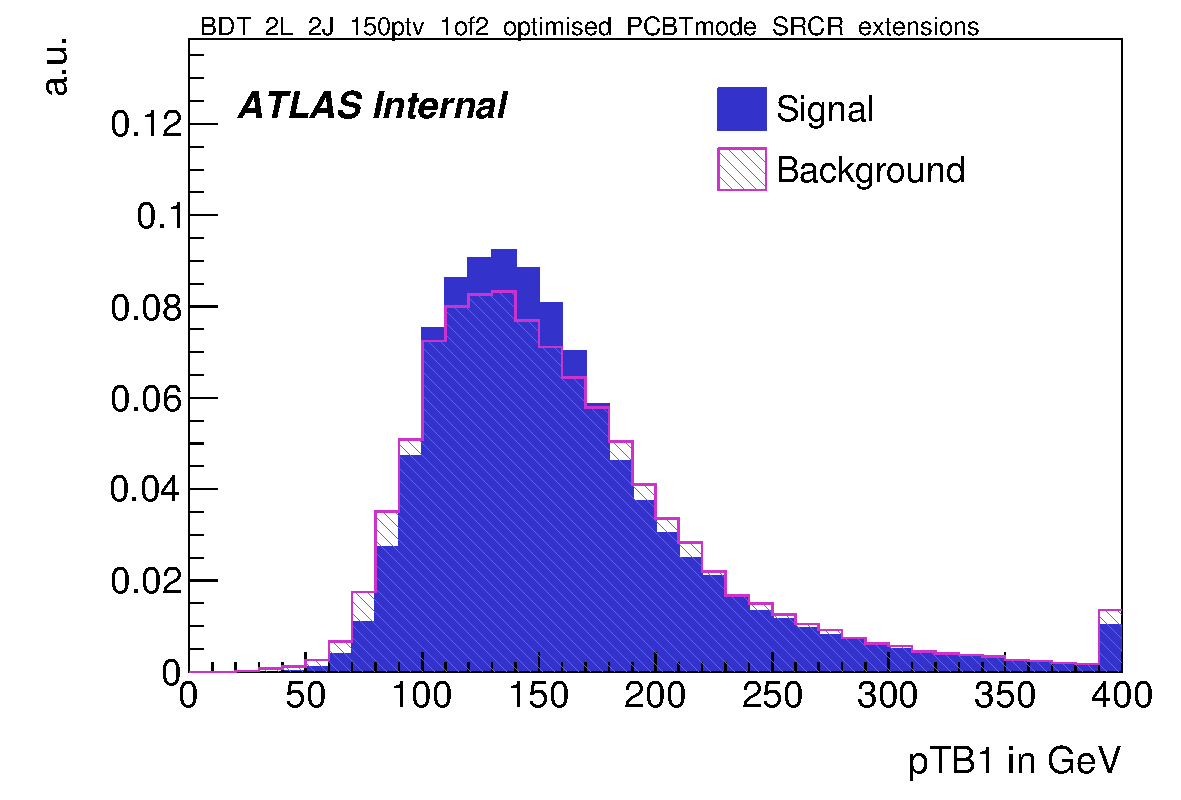
\includegraphics[width=0.33\linewidth]{2-lep-mva/Distr_SignalBackground_pTB1_BDT_2L_2J_150ptv_1of2_optimised_PCBTmode_SRCR_extensions-eps-converted-to}}          
    \subfloat[]{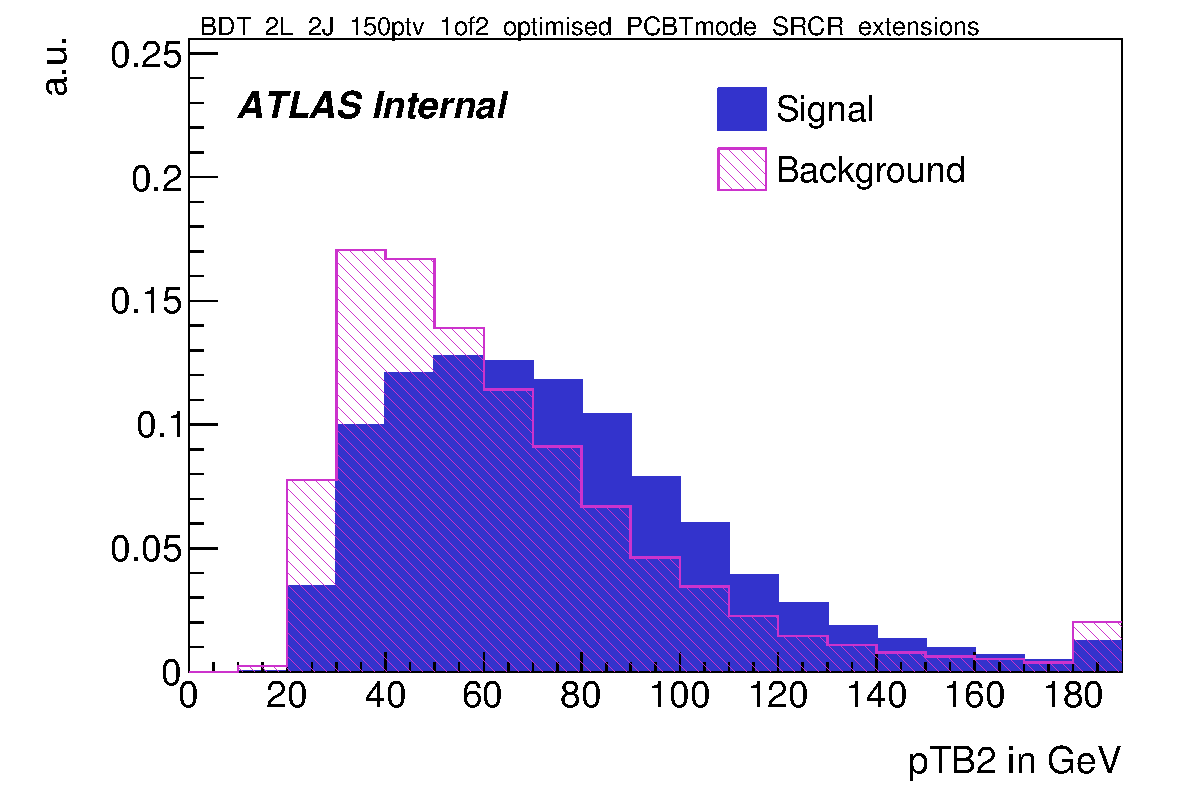
\includegraphics[width=0.33\linewidth]{2-lep-mva/Distr_SignalBackground_pTB2_BDT_2L_2J_150ptv_1of2_optimised_PCBTmode_SRCR_extensions-eps-converted-to}} \\
    \subfloat[]{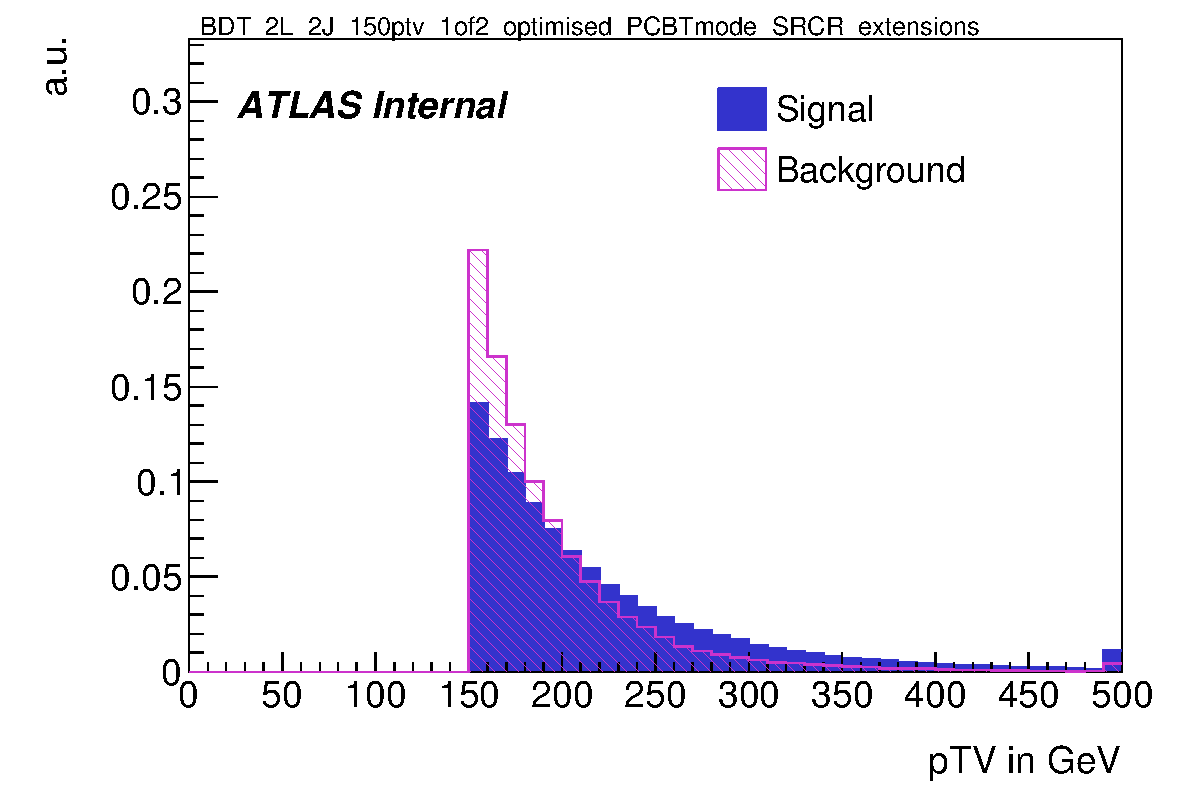
\includegraphics[width=0.33\linewidth]{2-lep-mva/Distr_SignalBackground_pTV_BDT_2L_2J_150ptv_1of2_optimised_PCBTmode_SRCR_extensions-eps-converted-to}}   
    \end{tabular}
    \caption[Inputs to the multi-variate analysis in the 2--lepton 2--jet
    region.]{Inputs to the multi-variate analysis in the 2--lepton 2--jet
      region. Signal events are shown in blue and background events are shown in
      red. The signal and background histograms have been normalised to the same
      area.The distributions only include events with $p_T^{Z}$ > 150
      \GeV.}
    \label{fig:bdtinputs-2lep}
\end{figure}


The BDT is designed to maximise the separation between signal and background
Monte-Carlo predictions. This does not take into account the statistical error
on the quantities of each bin in the discriminant distribution. To mitigate this
issue a transformation is applied, details of which are found in
appendix~\ref{app:bdt-transform}. The performance of the algorithm in terms of
over-fitting is found to be robust~\cite{VHMainNote2019} and the separation
between categories can be seen in section~\ref{sec:prefit}.

\section{Profile Likelihood Fit}%
\label{sec:plf}

Ultimately the results of the analysis come from a profile-likelihood fit. This
fit uses a binned likelihood function whose maximum corresponds to the best
agreement between data and the prediction. The likelihood is defined as the
product over all bins of the Poisson probability to observe $N^{\text{obs}}_i$
data events given a prediction of $N^{\text{pred}}_i(\mu,\bm{k},{\bm\theta})$
events in a given bin $i$,
\begin{equation} \mathcal{L}(\mu,{\bm{k},\bm{\theta}}) =
\prod_{i\in\,\text{bins}} \frac{\left( N_{i}^{\text{pred}}(\mu,{\bm{k,\theta}})
\right)^{N_{i}^{\text{data}}}}{N_{i}^{\text{data}}\,!} \cdot
e^{-N_{i}^{\text{pred}}(\mu,{\bm{k,\theta}})}.
  \label{eq:likelihood}
\end{equation} The number of predicted events $N^{\text{pred}}_i$ is dependent
on three sets of parameters, the signal strength $\mu$, the scale factors
$\bm{k}=\left\{k_1, ...,k_j\right\}$, and the nuisance parameters $\bm{\theta} =
\left\{\theta_1,...,\theta_l\right\}$, as follows
\begin{equation} N_{i}^{\text{pred}}(\mu,\bm{k},\bm{\theta}) = \mu \cdot
N_{i,\text{sig}}^{\text{pred}}(\bm{\theta}) + \sum_{b\in\,\text{bkg}} k_b\cdot
N_{i,b}^{\text{pred}}(\bm{\theta}).
\end{equation} The ratio between the measured and the expected signal
cross-sections $\mu=\sigma/\sigma_{\text{SM}}$, known as the signal strength, is
the parameter of interest in the nominal fit. It is common to all analysis
regions that enter into the fit. Each of the scale factors $k_j$ and the signal
strength scale either their associated quantity linearly without any prior
constraint or penalty in the likelihood function, in further sections these
parameters will be referred to as floating. Each nuisance parameter $\theta_i$
encodes the dependence of the prediction on systematic uncertainties into
continuous parameters in the likelihood. Prior knowledge of the uncertainty that
these parameters encode for is expressed as a Gaussian penalty term
$\mathcal{G}(0\,|\,\theta_i,1)$ added to the likelihood for each uncertainty.
The parameters $\theta_i$ are therefore expressed as a number of standard
deviations of a unit Gaussian in the subsequent sections. These penalties
results in a log-normal, or normal dependence of the predicted yields or shapes
on the displayed parameter values.

The nominal fit result in terms of $\mu$ and $\sigma_{\mu}$ is obtained by
maximizing the likelihood function with respect to all parameters. This is
referred to as the maximized log-likelihood value, MLL. The profile likelihood
ratio test statistic, $q_\mu$, is then constructed as follows:
\begin{equation} q_\mu = - 2\; \ln \left[ \mathcal{L} (\mu,
\hat{\hat{\mathbf{k}}}, \hat{\hat{\bm\theta}}_{\mu})\, / \, \mathcal{L}
(\hat{\mu}, \hat{\mathbf{k}}, \hat{\bm\theta}) \right]
\end{equation} where $\hat{\mu}$ and $\hat{\theta}$ are the parameters that
maximise the likelihood (with the constraint $0 \leq \hat{\mu} \leq \mu$), and
$\hat{\hat{\theta}}_\mu$ are the nuisance parameter values that maximise the
likelihood for a given $\mu$. This test statistic is used to measure the
compatibility of the background only model with the observed data.

\subsection{STXS Measurements}

As well as the single parameter of interest mode described above the fit can
also be run in a multiple parameter of interest paradigm. The purpose of this
fit is to measure the cross-section of the \WH\ and \ZH\ processes in a number
of well defined regions of phase space. In order to achieve this a simplified
template cross-section (STXS) scheme is used. As in the previous
measurement~\cite{STXSpaper} the STXS bins are split into many categories before
being merged down to include $p_{\mathrm{T}}^V$ bins of 75--150~\GeV,
150--250~\GeV\ and >250~\GeV. The 75--150~\GeV\ bin does not include a
measurement of \WH\ as there is no 75--150~\GeV\ bin available in the 1--lepton
channel and so there ought not to be any signal events present in this region of
phase space.

\section{Pre-fit Data Versus Prediction}
\label{sec:prefit}

This section shows the pre-fit distributions of the Monte-Carlo prediction
versus the data in every analysis region that enters into the profile-likelihood
fit. Figures~\ref{fig:0lep-sr-prefit},~\ref{fig:1lep-sr-prefit}
and~\ref{fig:2lep-sr-prefit} show the distributions in the signal regions of the
0--, 1-- and 2--lepton channels respectively. Plots of all distributions in all
regions can be found in appendix~\ref{app:full-prefit}.
\begin{figure}[hb]
  \centering
  \begin{tabular}{cc}
    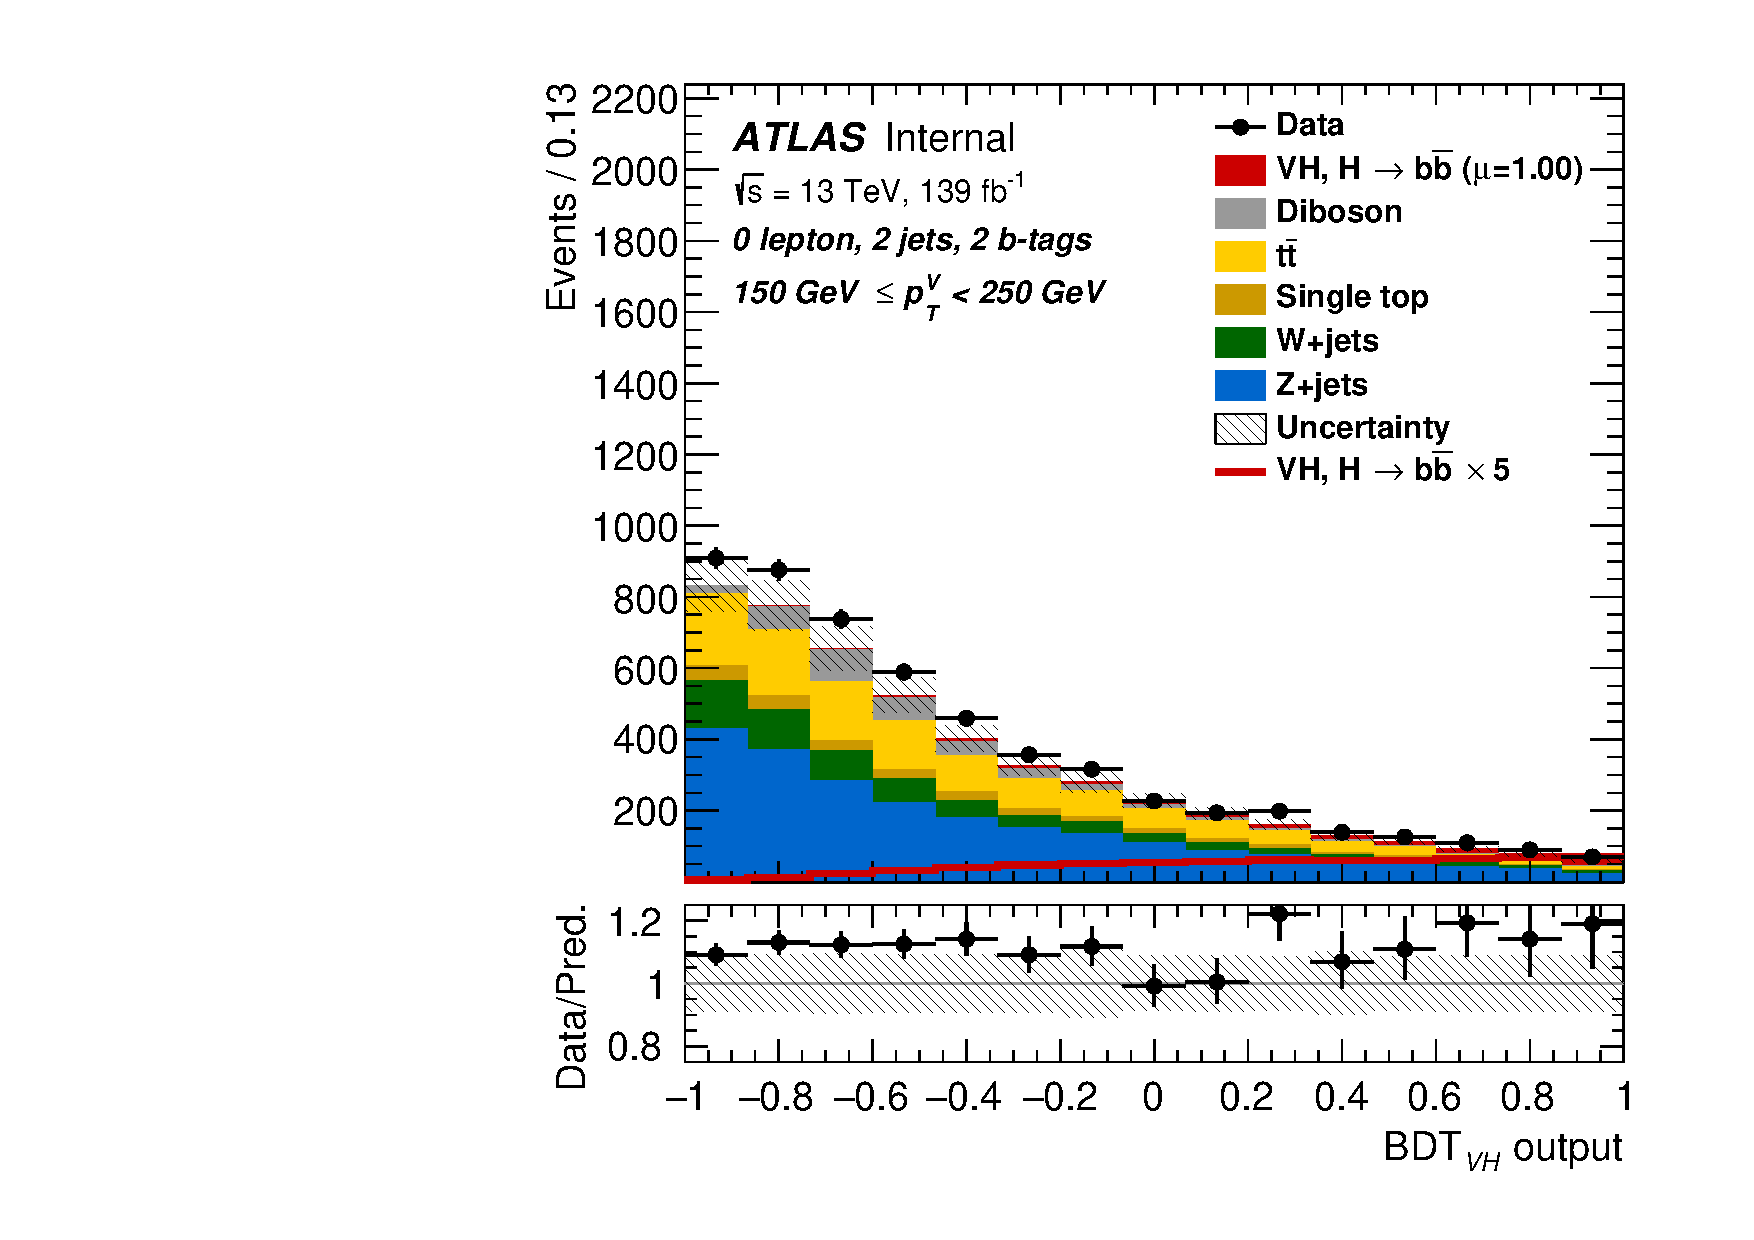
\includegraphics[width=.49\textwidth]{final_fit_mva/prefit/Region_BMax250_BMin150_Y6051_DSR_T2_L0_distmva_J2_Prefit}%
    & 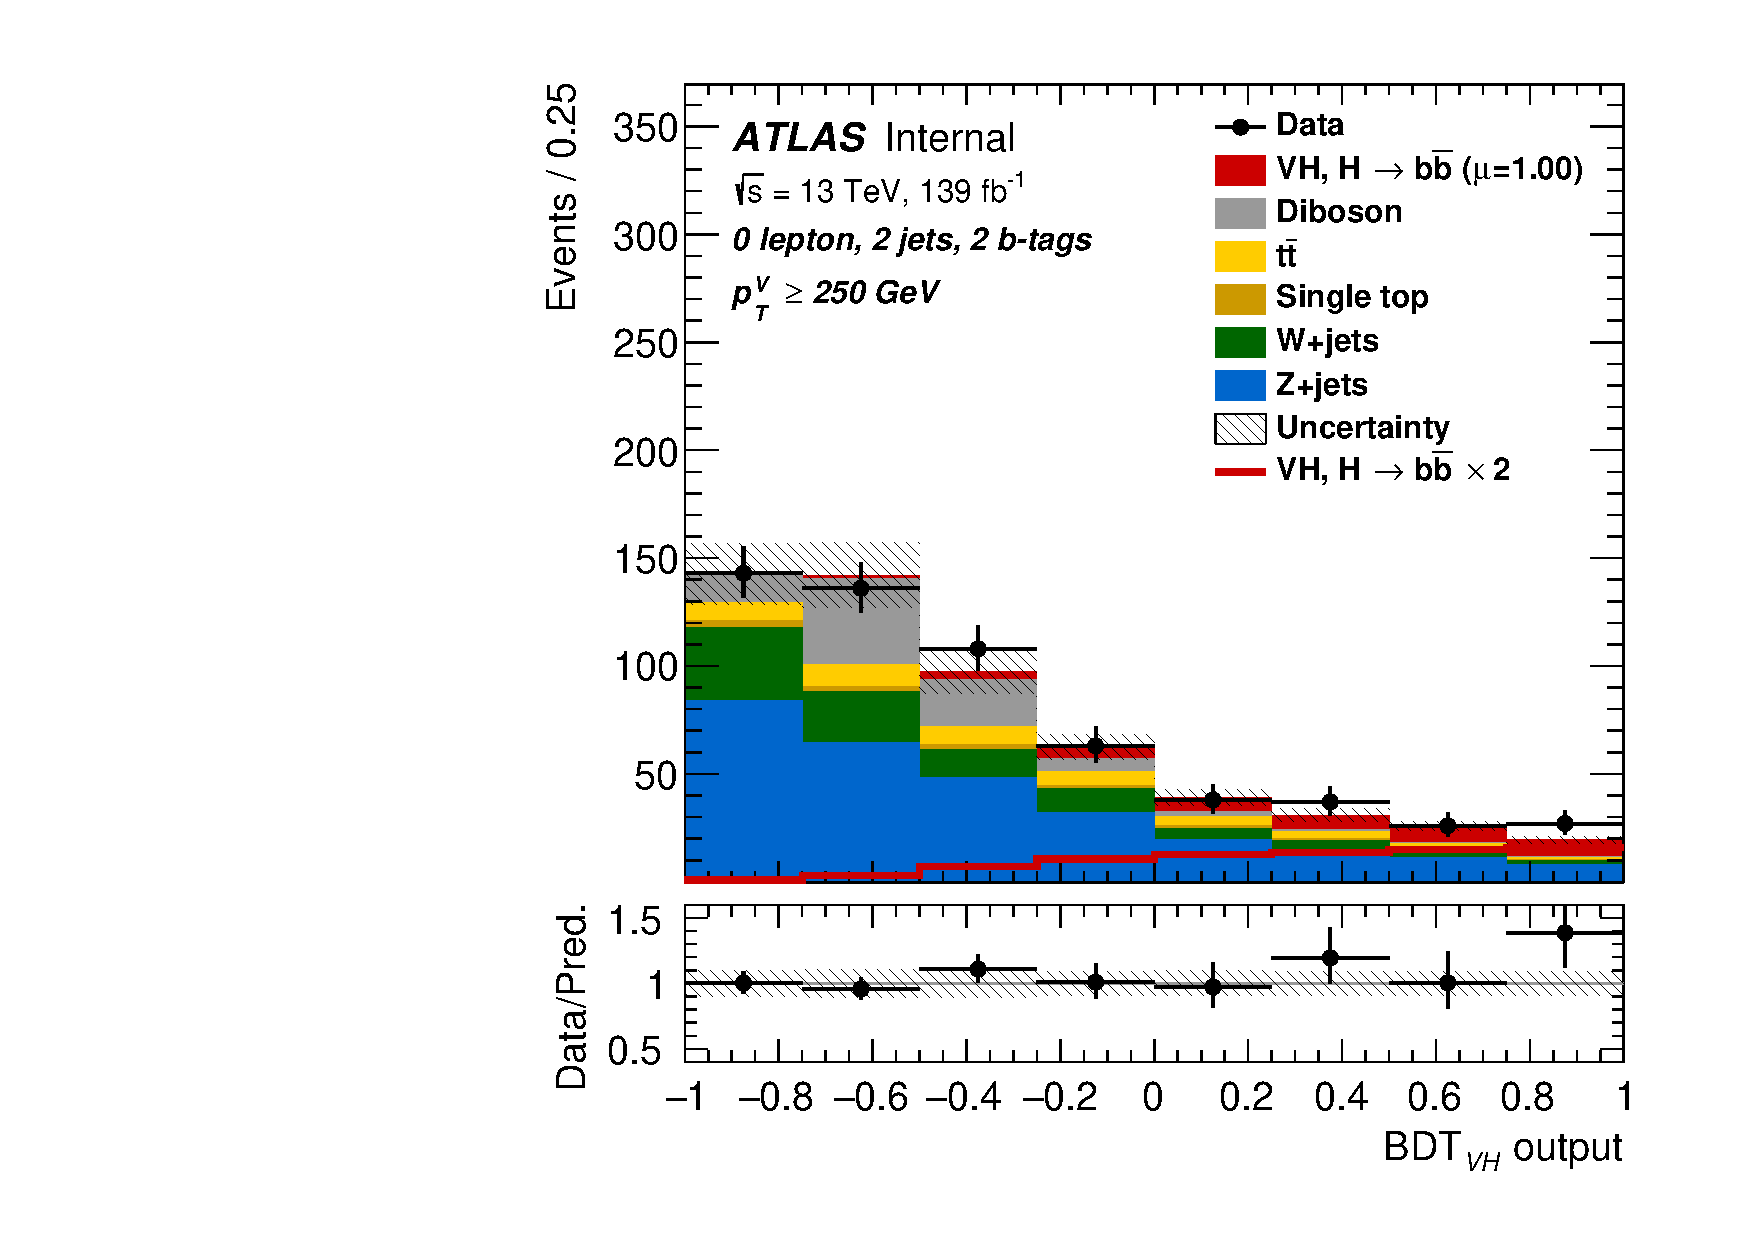
\includegraphics[width=.49\textwidth]{final_fit_mva/prefit/Region_BMin250_Y6051_DSR_T2_L0_distmva_J2_Prefit} \\
    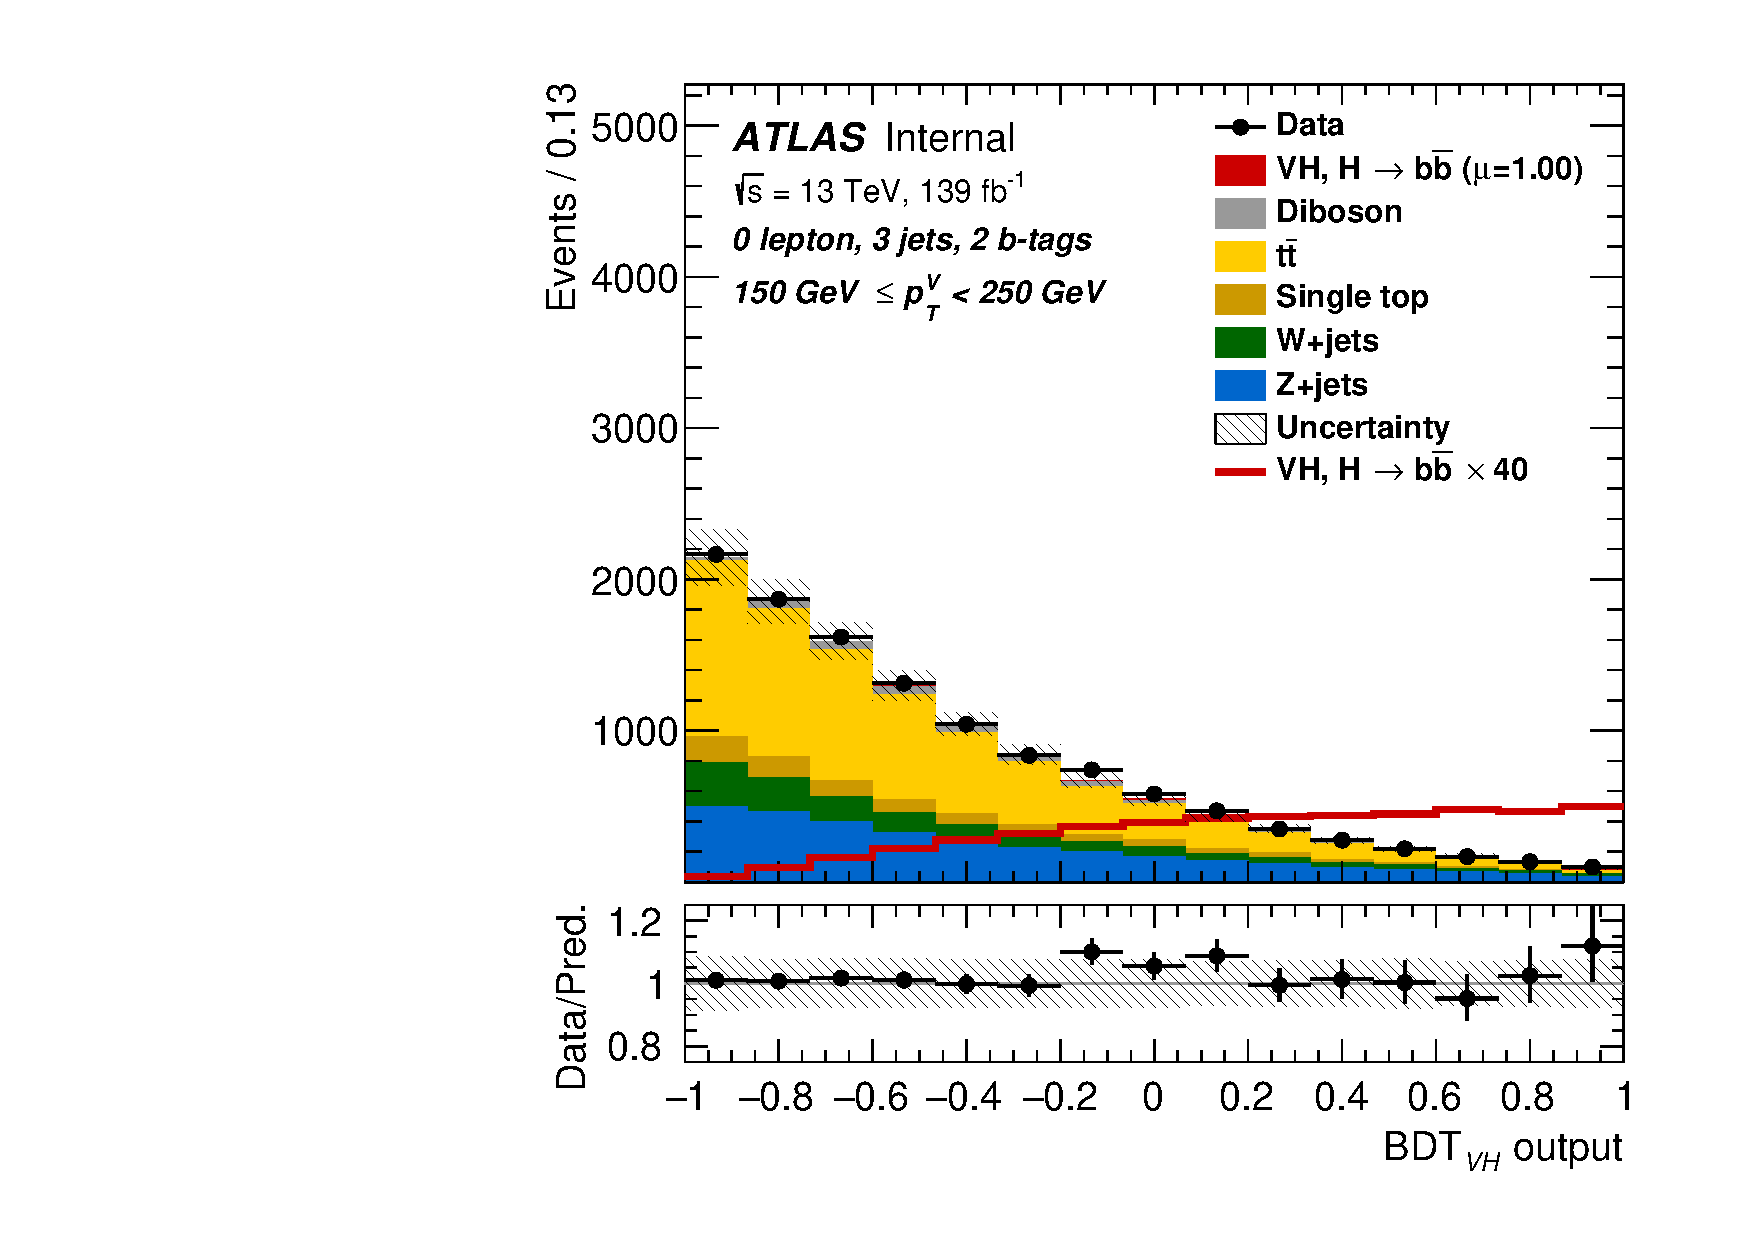
\includegraphics[width=.49\textwidth]{final_fit_mva/prefit/Region_BMax250_BMin150_Y6051_DSR_T2_L0_distmva_J3_Prefit}%
    & 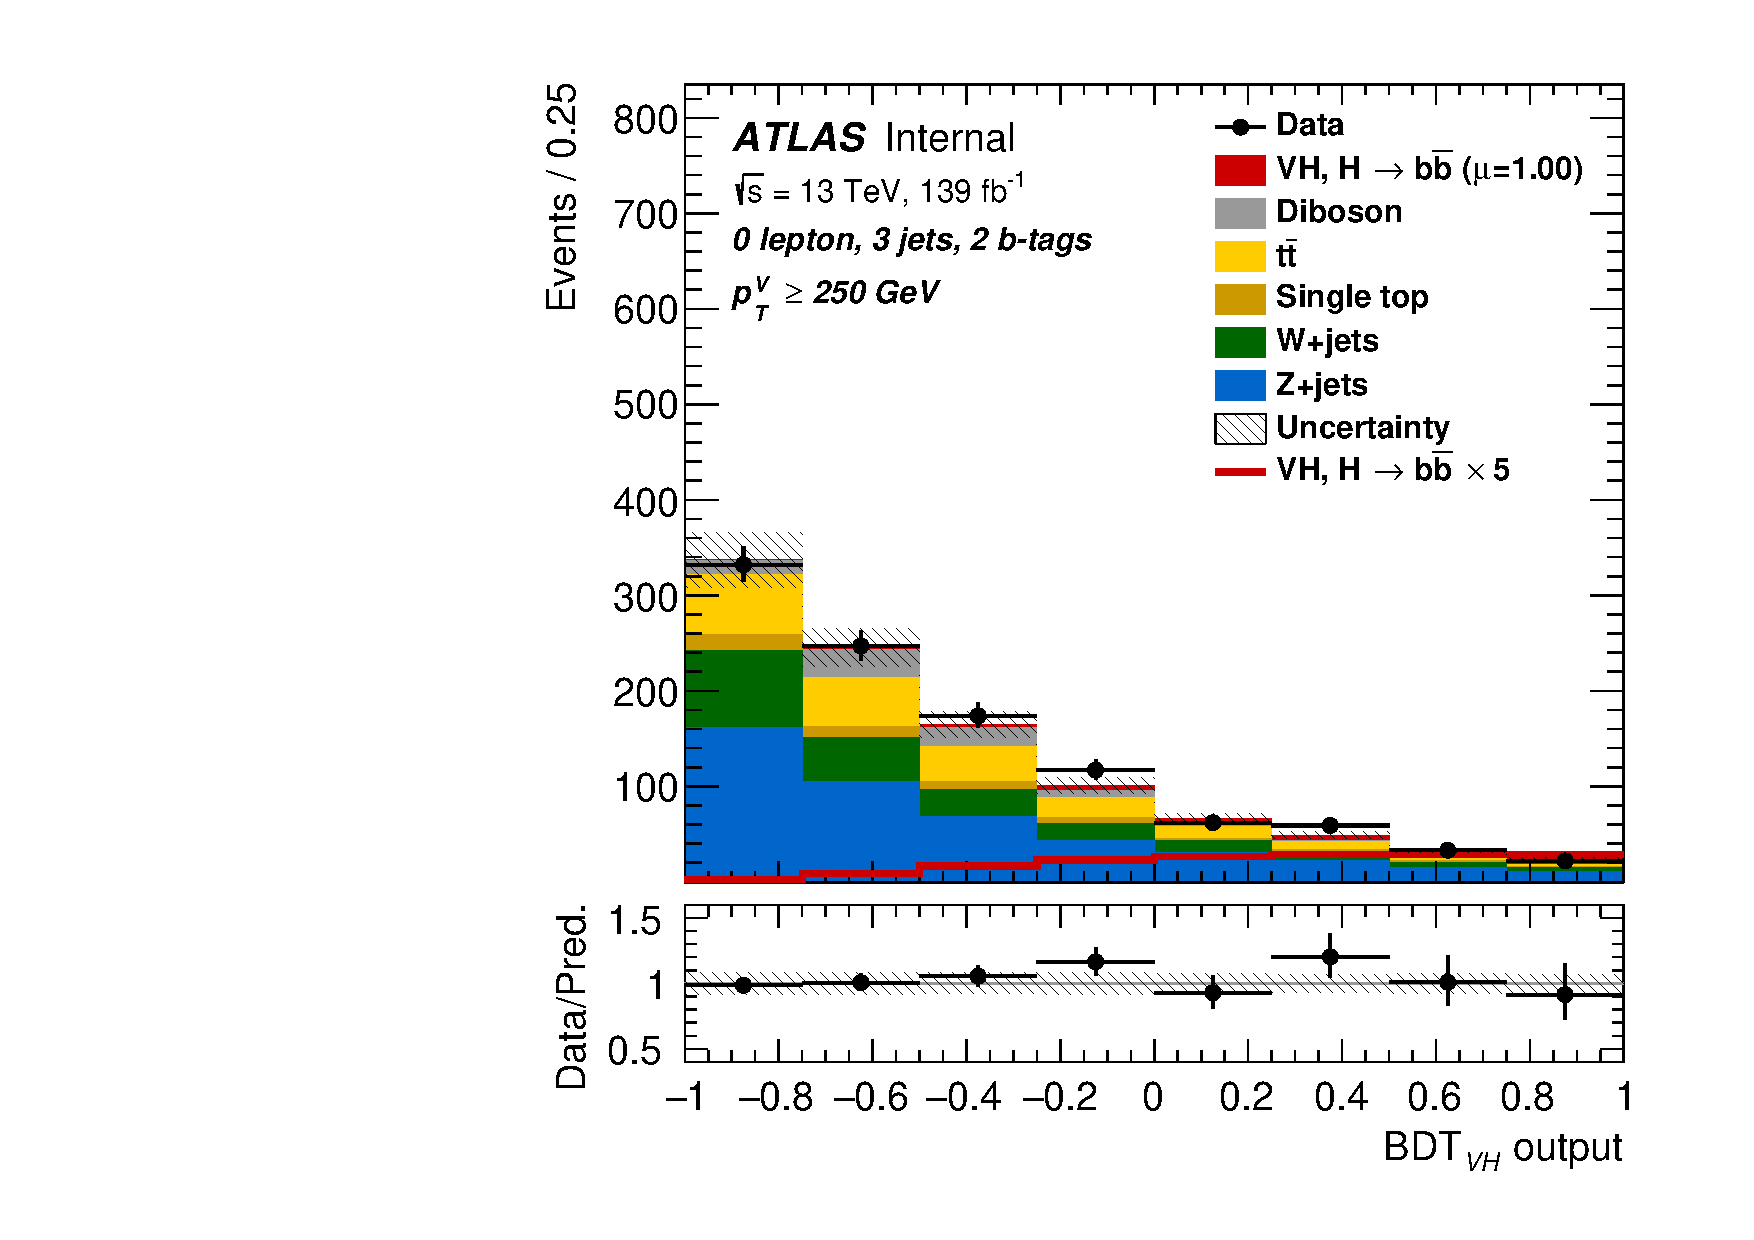
\includegraphics[width=.49\textwidth]{final_fit_mva/prefit/Region_BMin250_Y6051_DSR_T2_L0_distmva_J3_Prefit} \\
  \end{tabular}
  \caption{Pre-fit distributions in the signal region of the 0--lepton channel.}
  \label{fig:0lep-sr-prefit}
\end{figure}
\begin{figure}[hb]
  \centering
  \begin{tabular}{cc}
    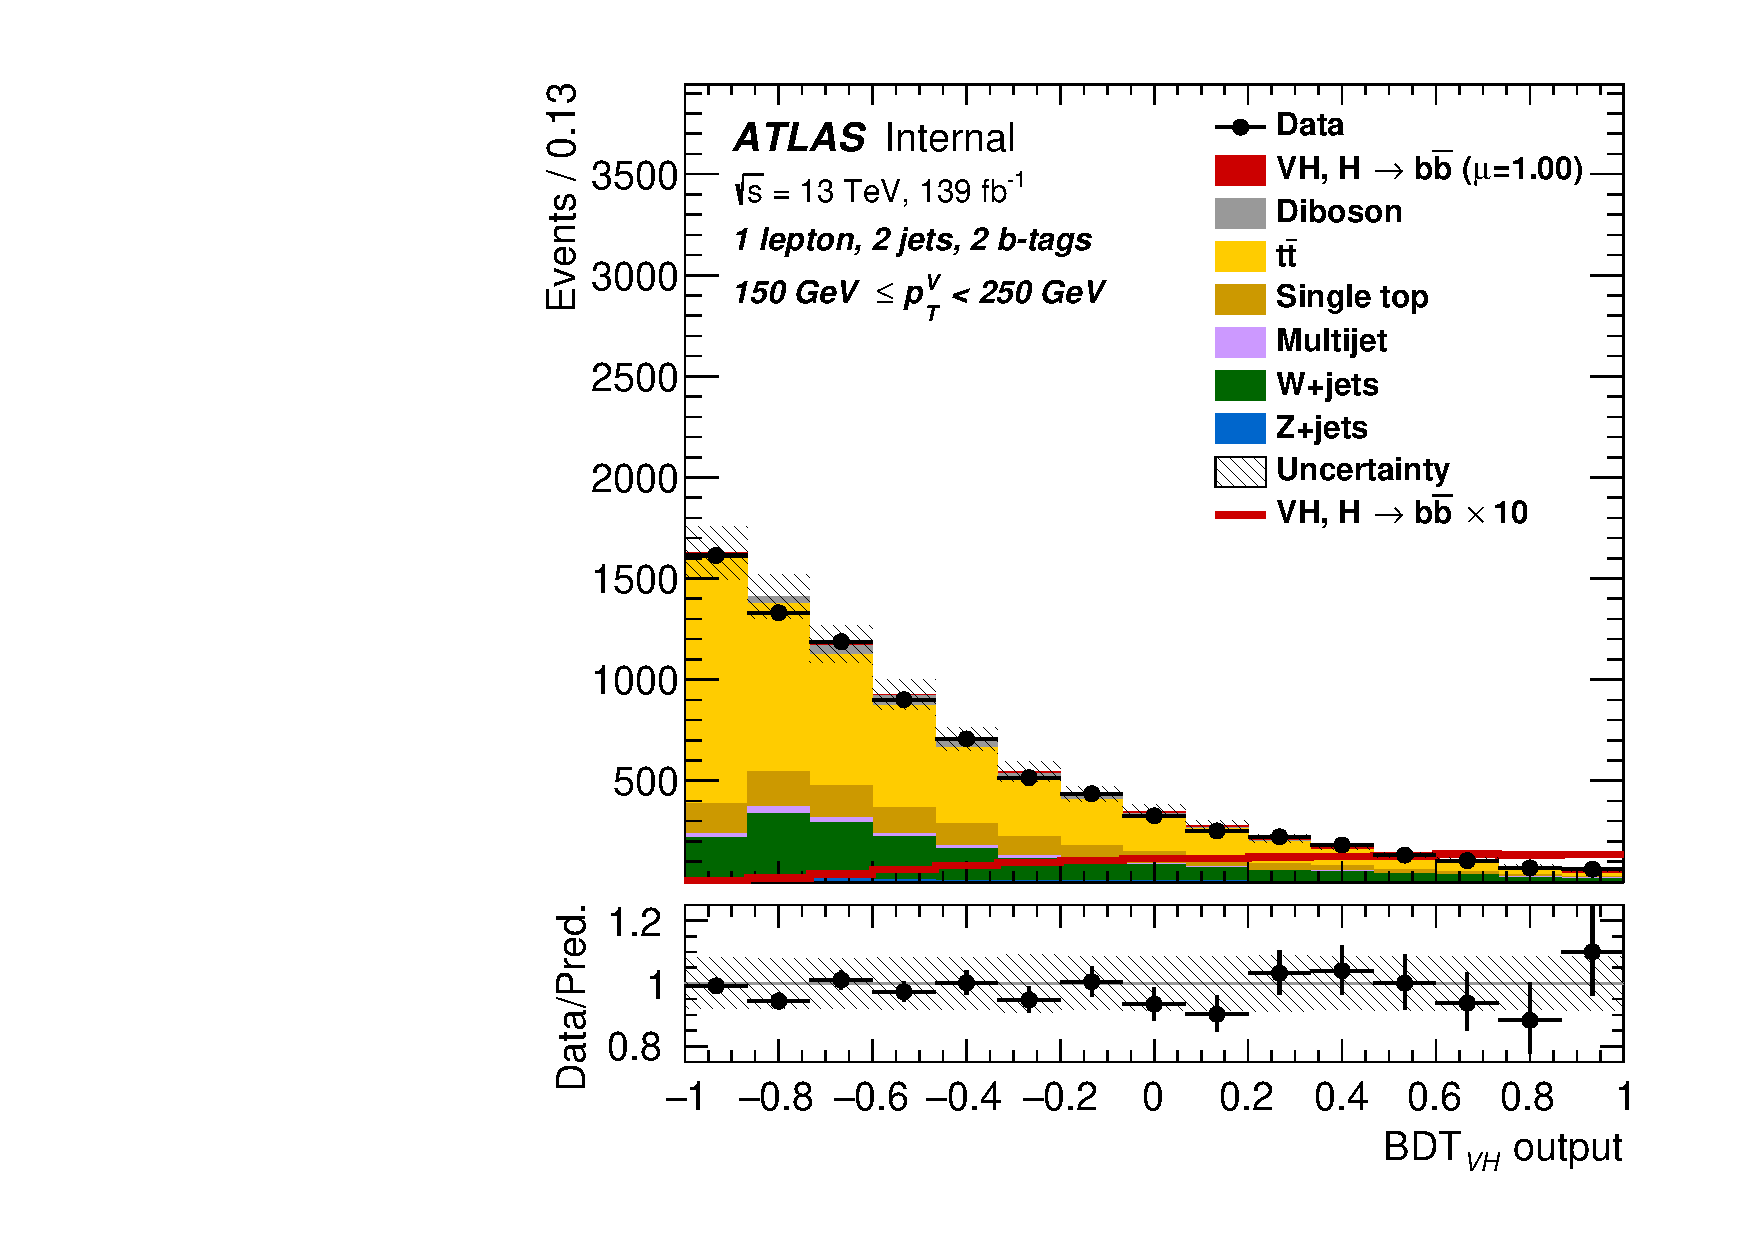
\includegraphics[width=.49\textwidth]{final_fit_mva/prefit/Region_BMax250_BMin150_Y6051_DSR_T2_L1_distmva_J2_Prefit}%
    & 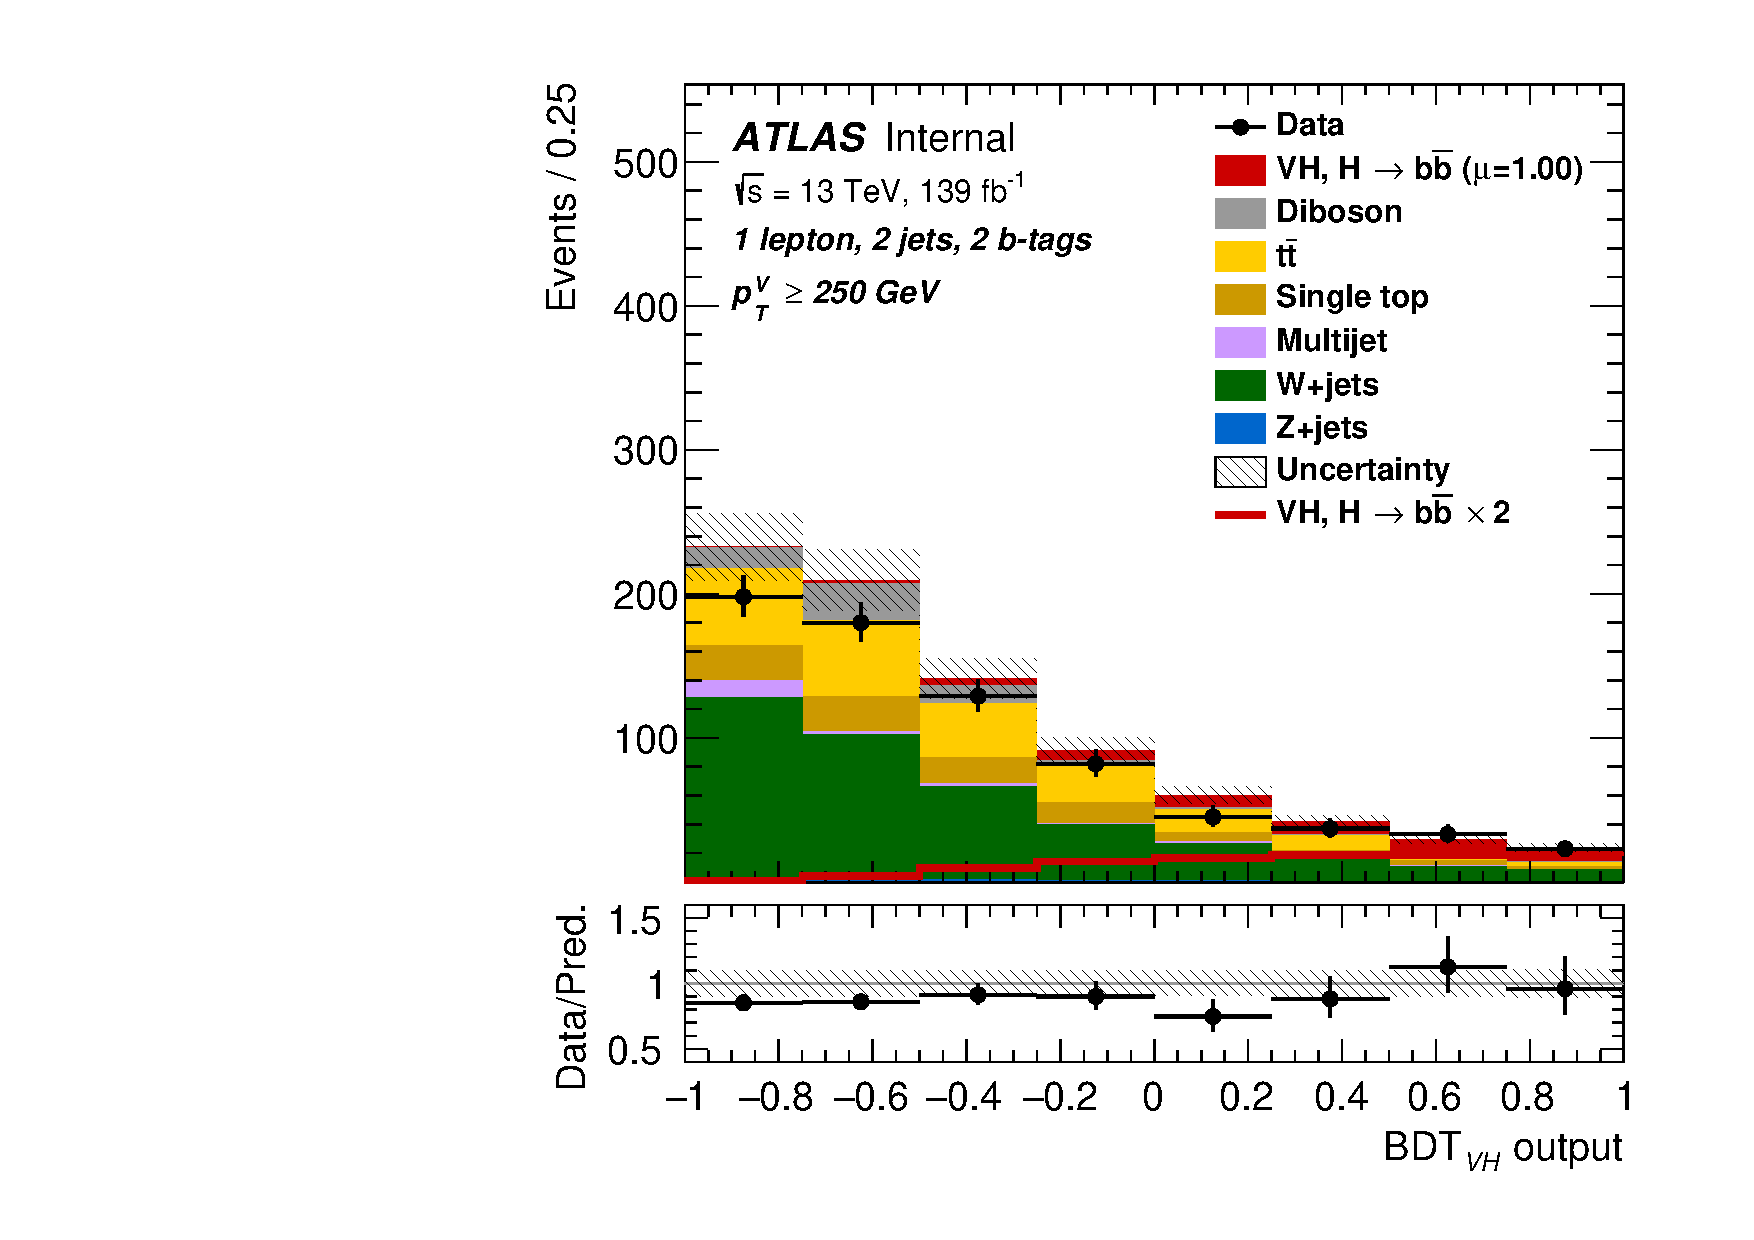
\includegraphics[width=.49\textwidth]{final_fit_mva/prefit/Region_BMin250_Y6051_DSR_T2_L1_distmva_J2_Prefit} \\
    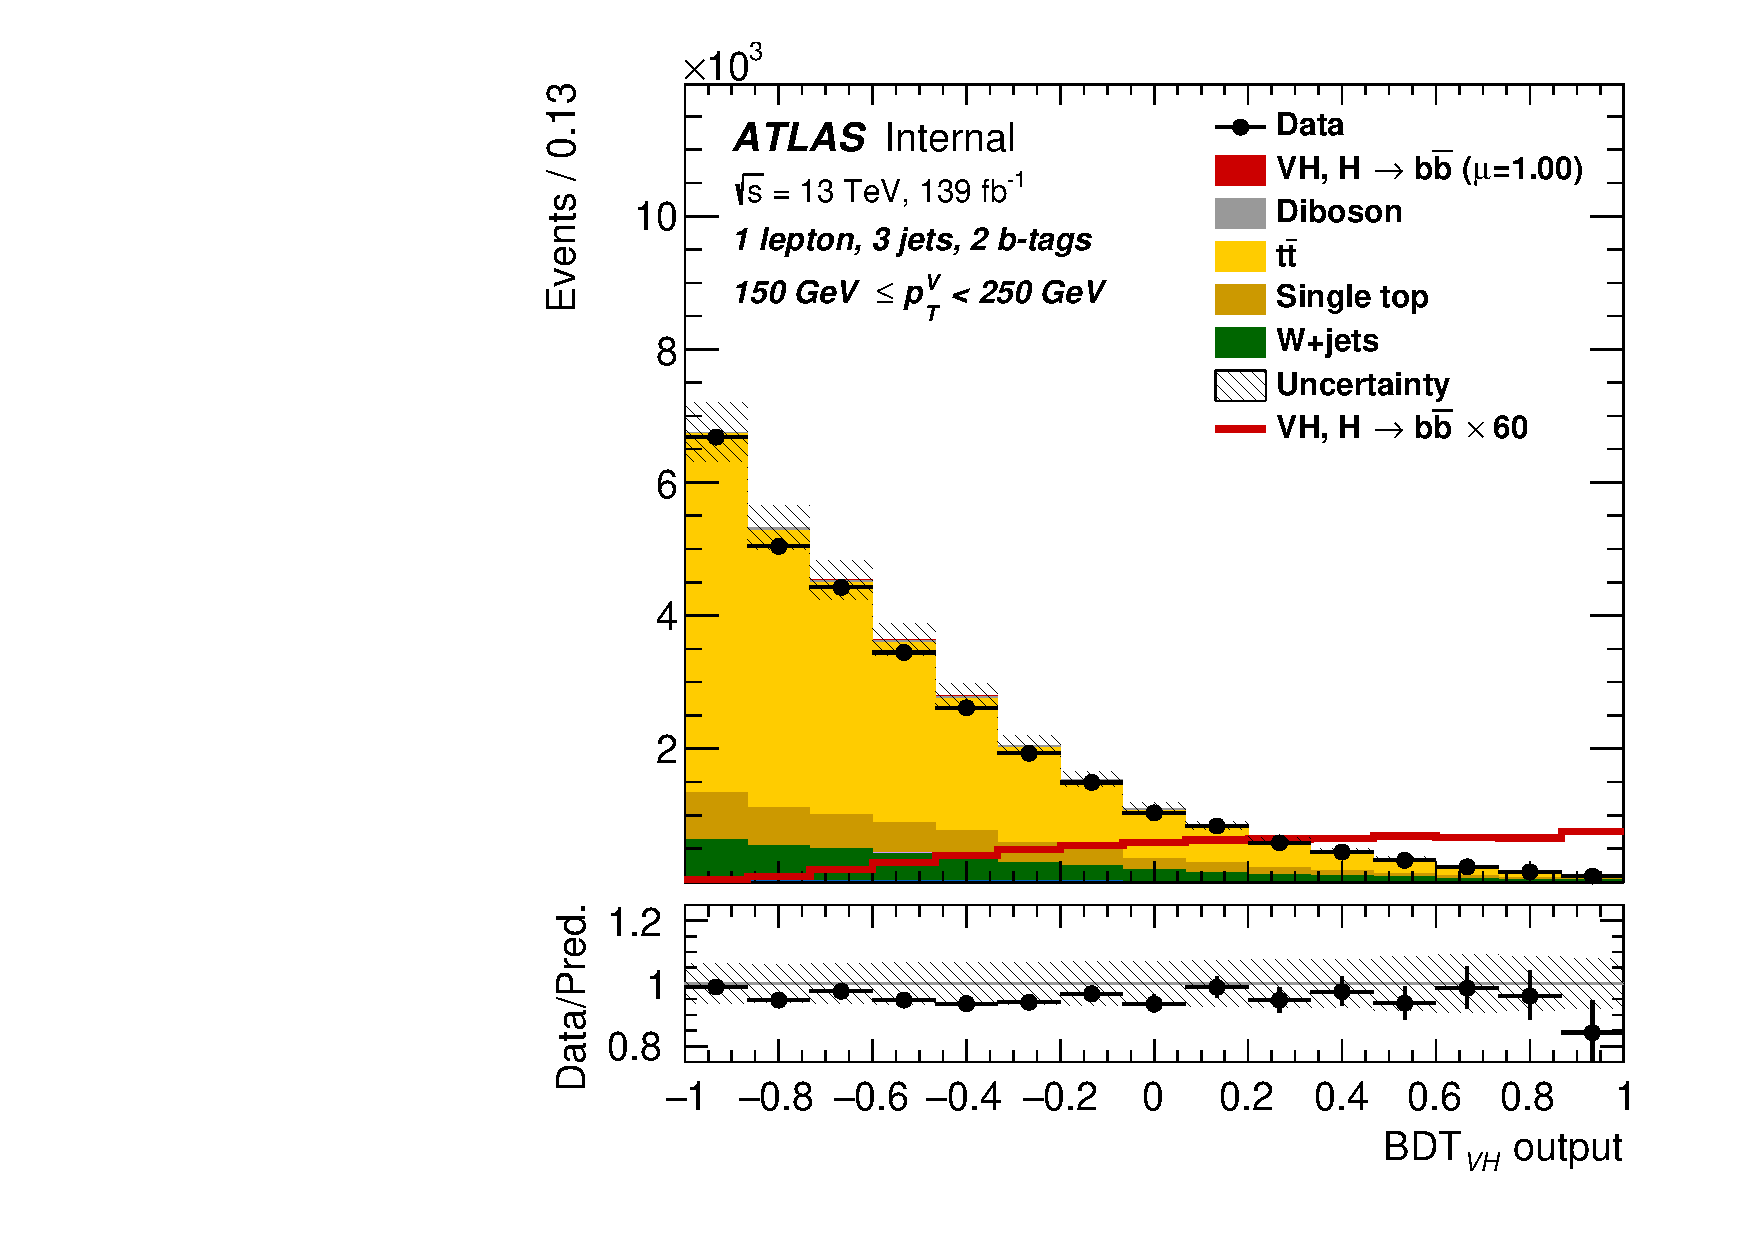
\includegraphics[width=.49\textwidth]{final_fit_mva/prefit/Region_BMax250_BMin150_Y6051_DSR_T2_L1_distmva_J3_Prefit}%
    & 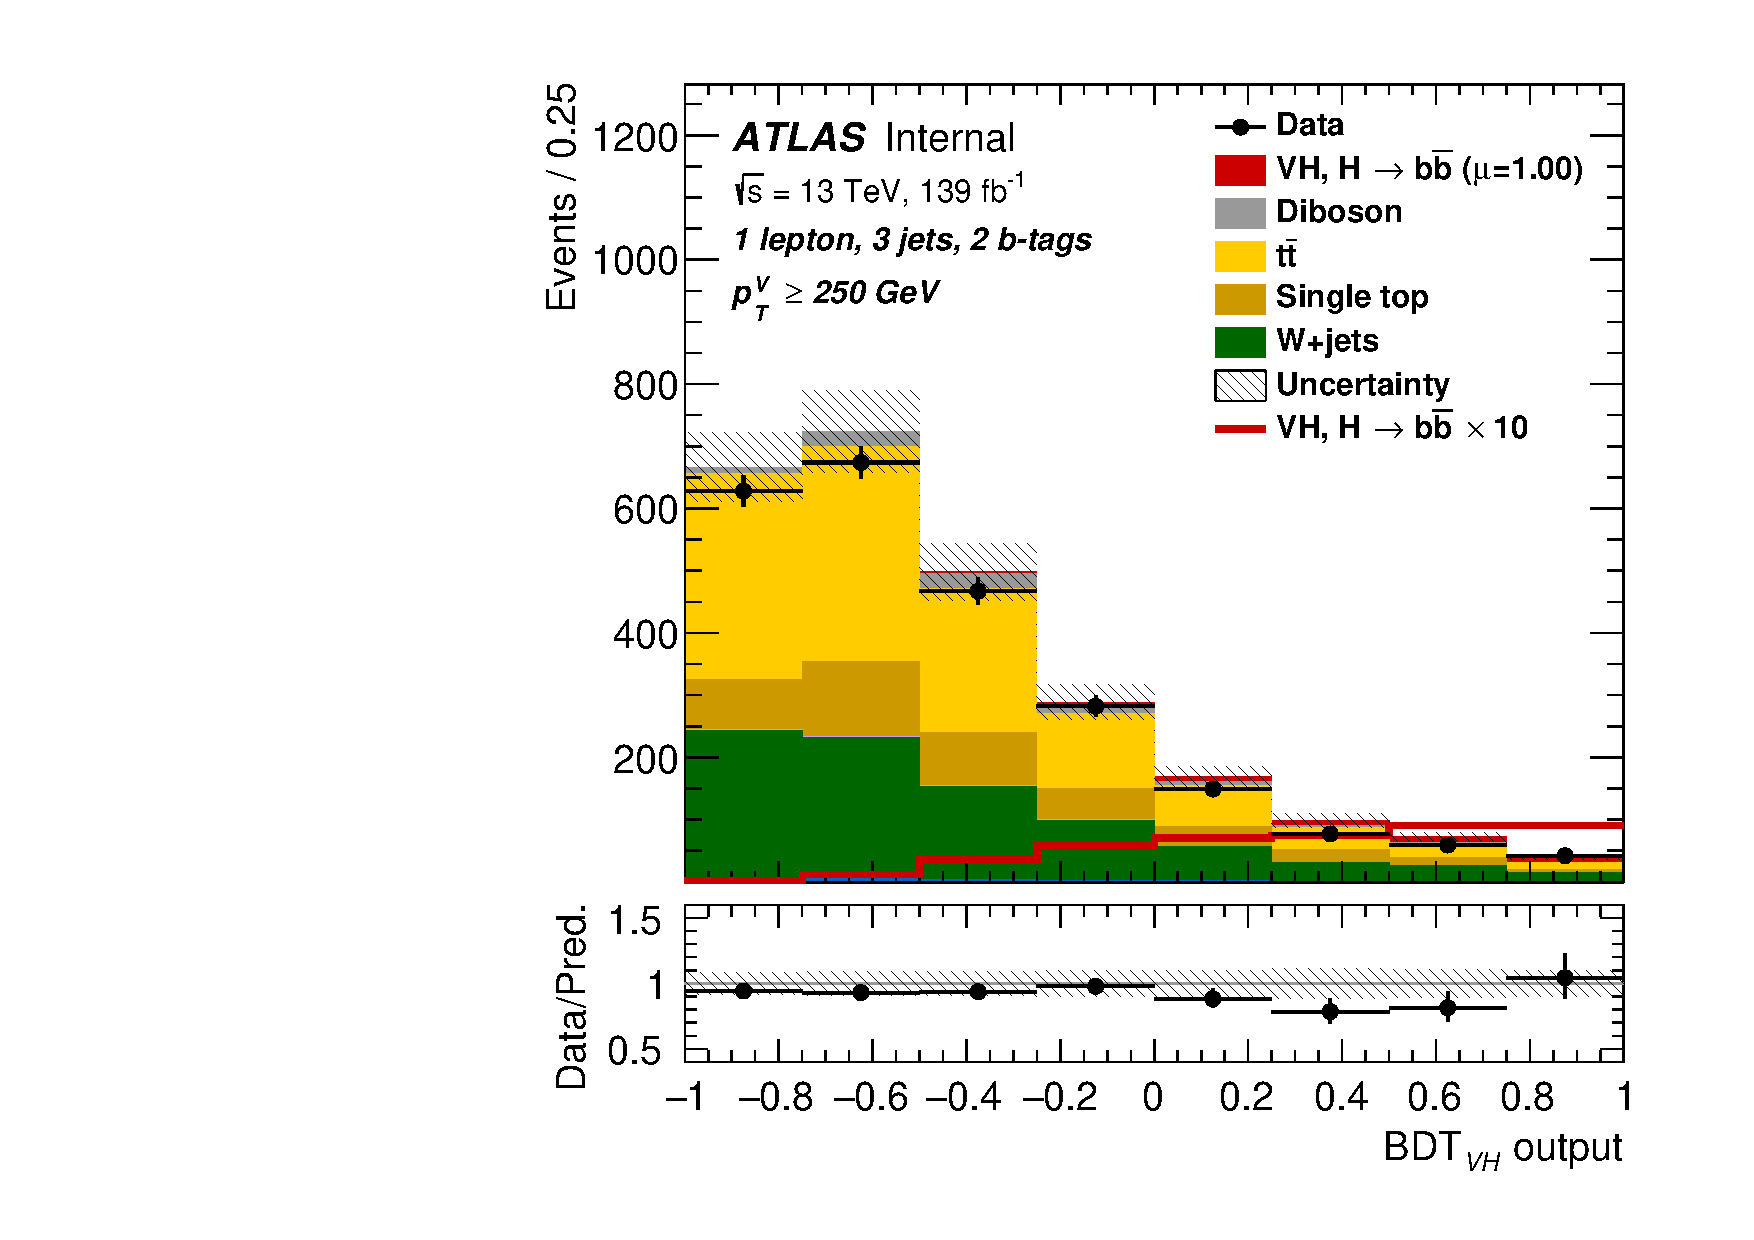
\includegraphics[width=.49\textwidth]{final_fit_mva/prefit/Region_BMin250_Y6051_DSR_T2_L1_distmva_J3_Prefit} \\
  \end{tabular}
  \caption{Pre-fit distributions in the signal region of the 1--lepton channel.}
  \label{fig:1lep-sr-prefit}
\end{figure}
\begin{figure}[hb]
  \centering
  \begin{tabular}{cc}
    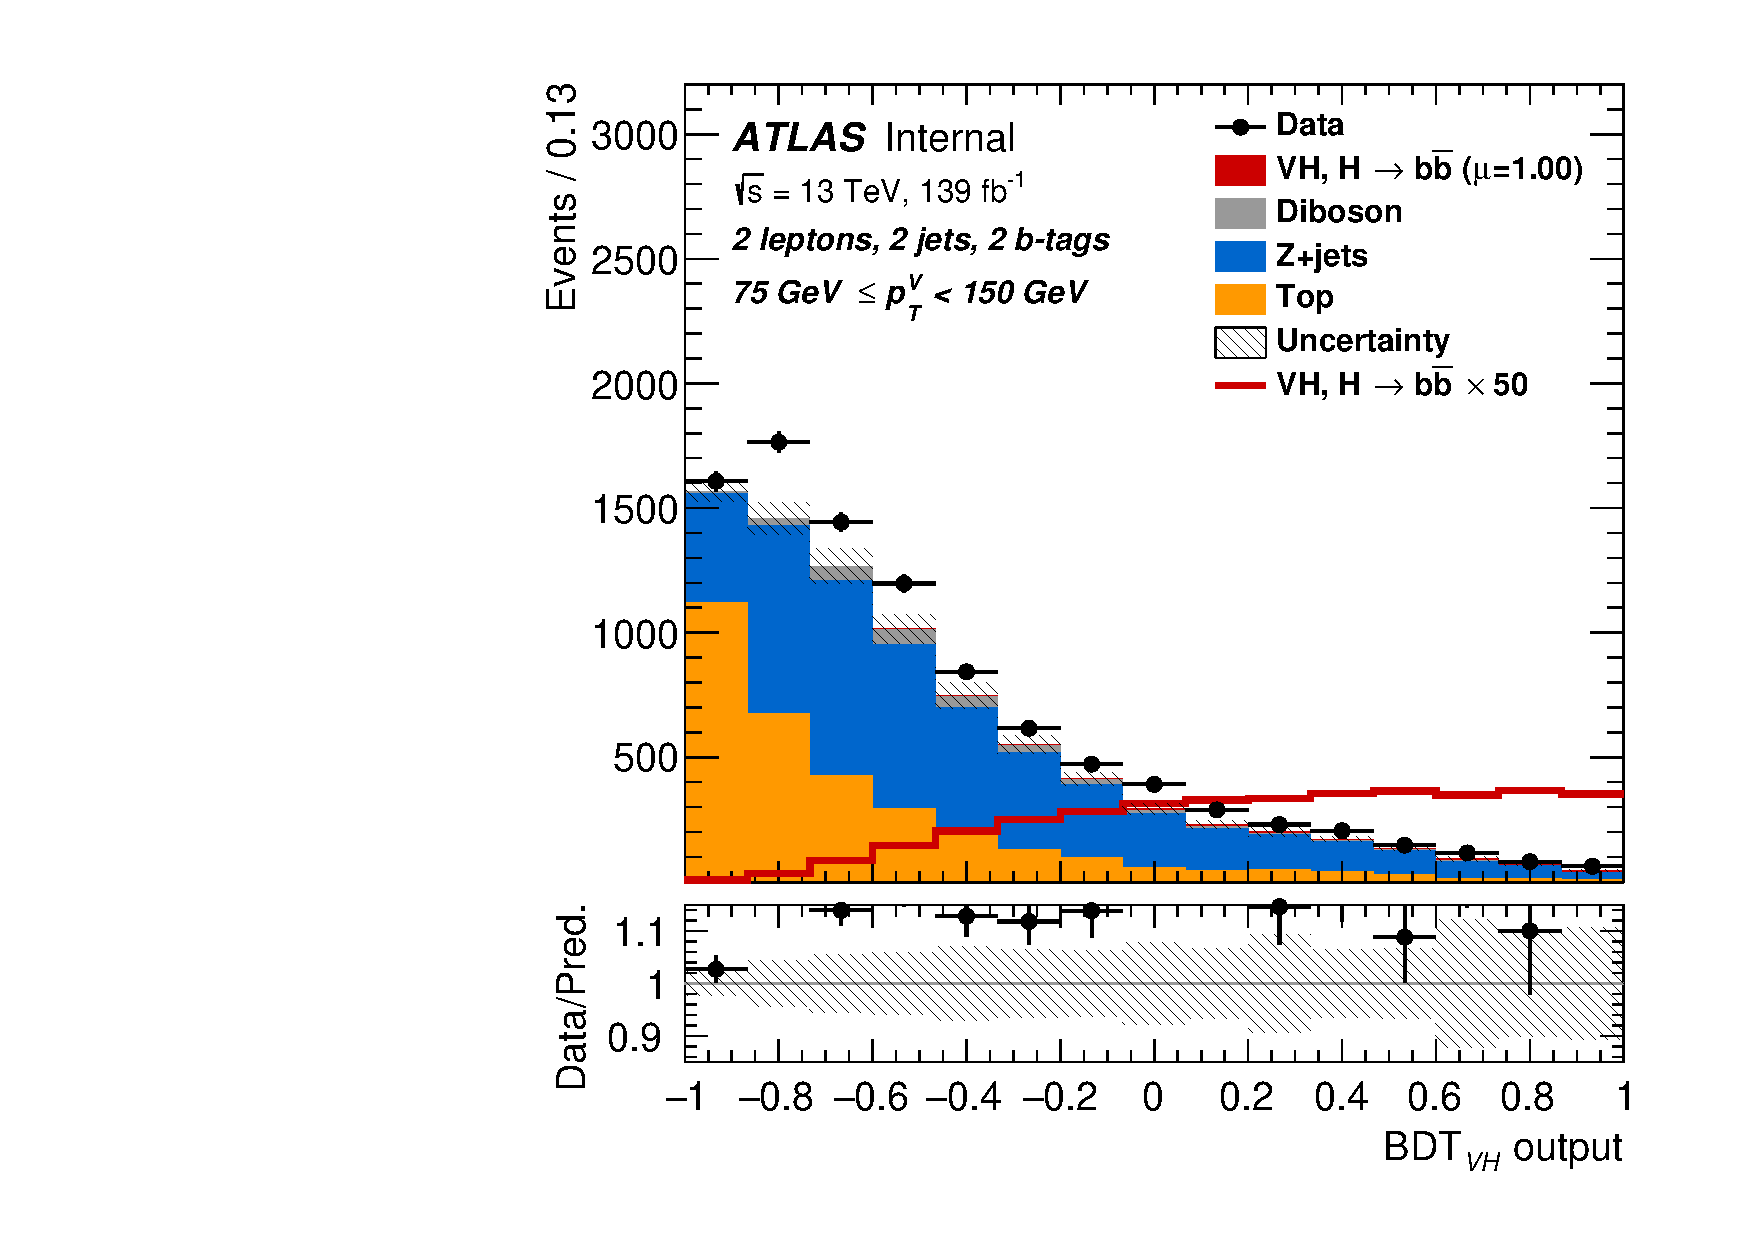
\includegraphics[width=.49\textwidth]{final_fit_mva/prefit/Region_BMax150_BMin75_Y6051_DSR_T2_L2_distmva_J2_Prefit}&
    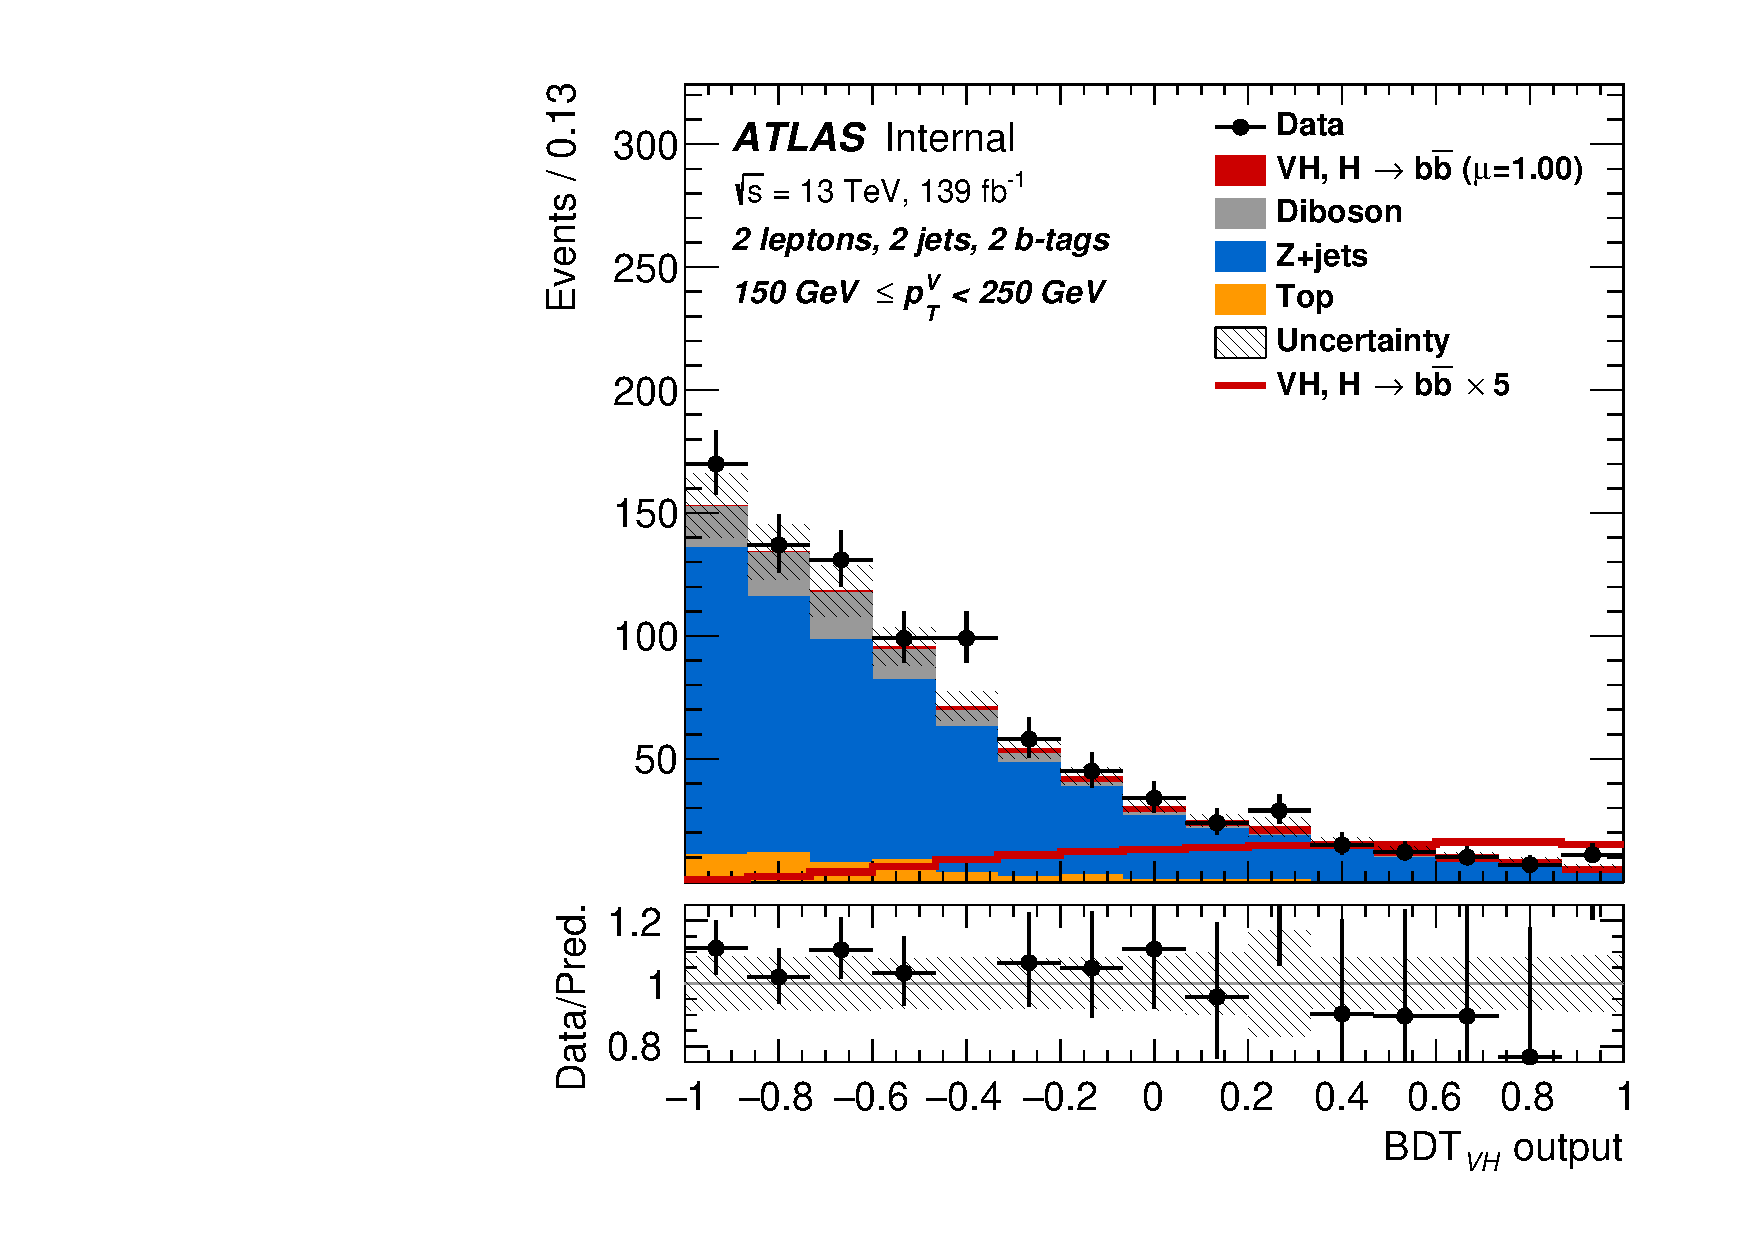
\includegraphics[width=.49\textwidth]{final_fit_mva/prefit/Region_BMax250_BMin150_Y6051_DSR_T2_L2_distmva_J2_Prefit}\\
    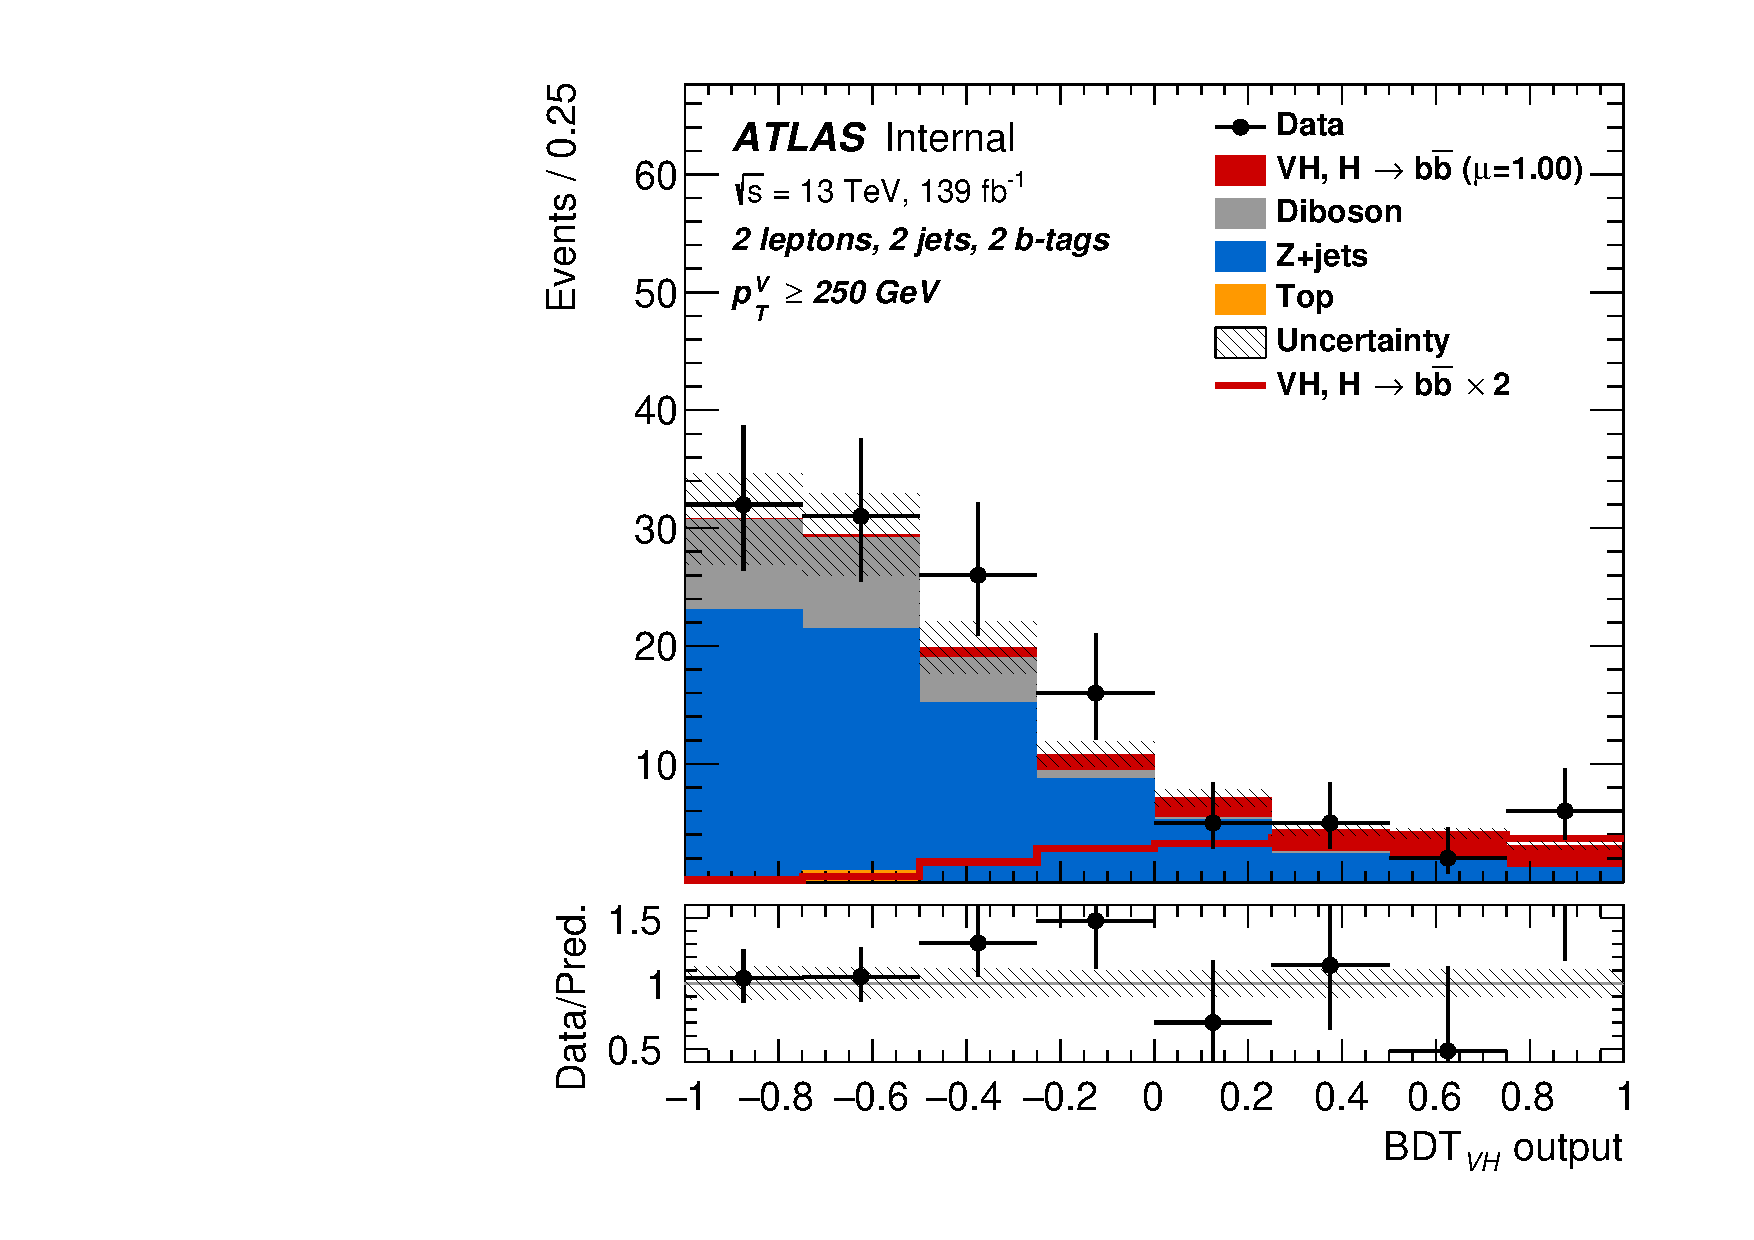
\includegraphics[width=.49\textwidth]{final_fit_mva/prefit/Region_BMin250_Y6051_DSR_T2_L2_distmva_J2_Prefit}&
    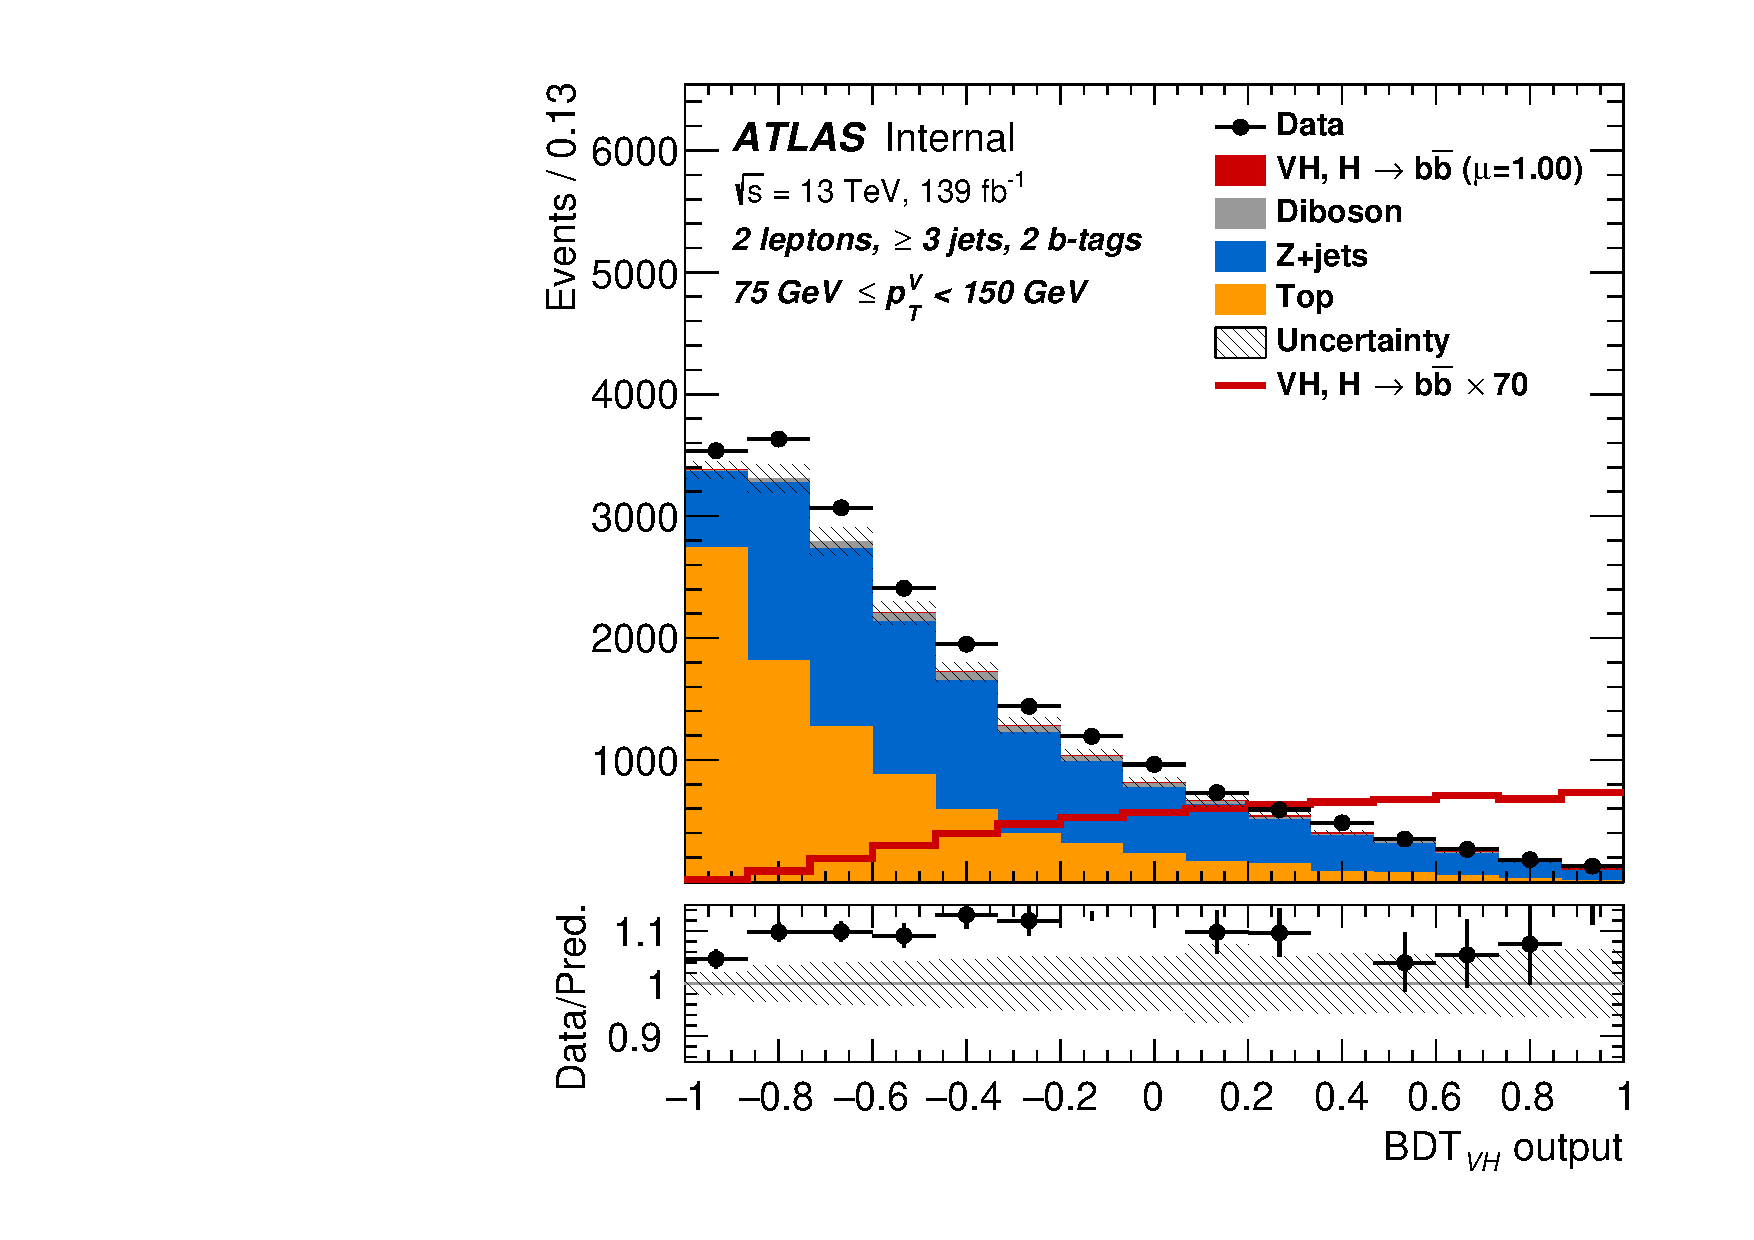
\includegraphics[width=.49\textwidth]{final_fit_mva/prefit/Region_BMax150_BMin75_incJet1_Y6051_DSR_T2_L2_distmva_J3_Prefit}\\%
    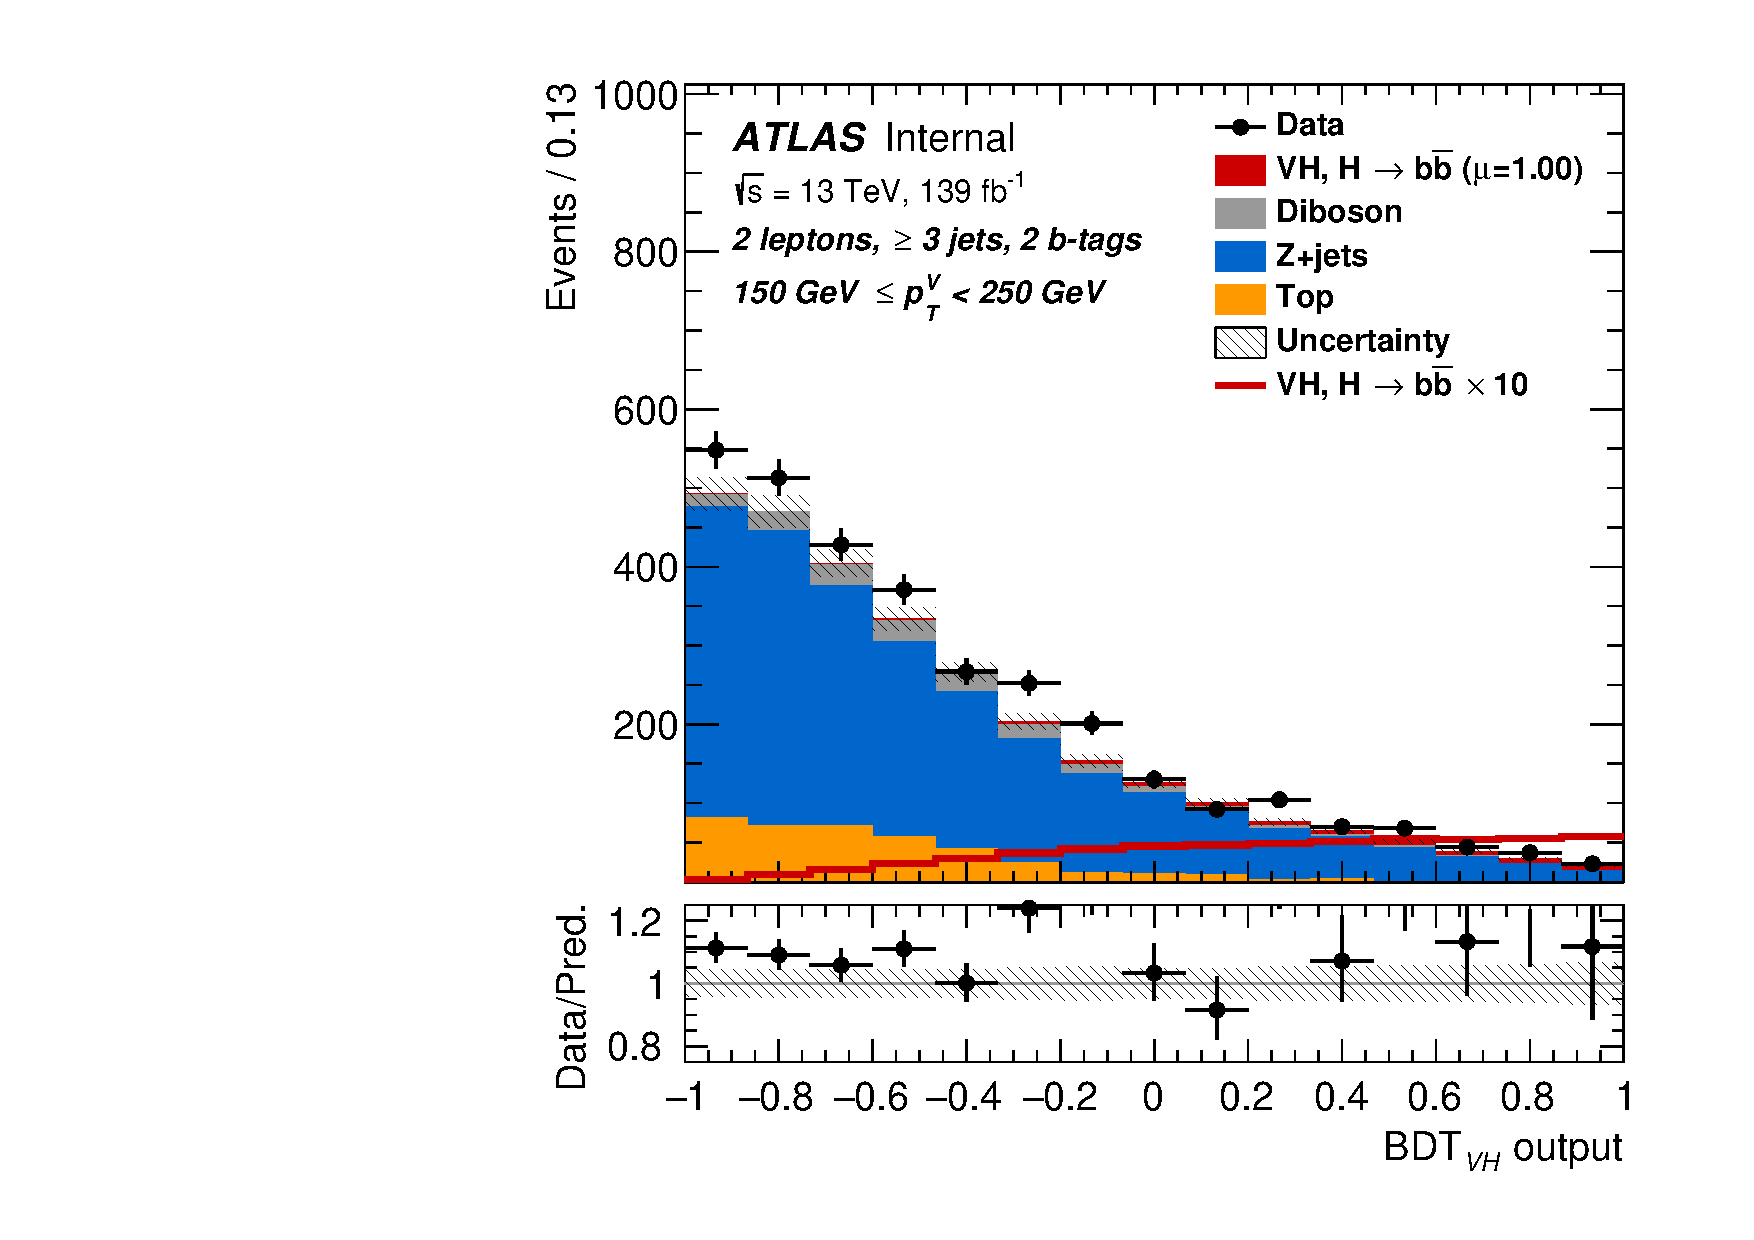
\includegraphics[width=.49\textwidth]{final_fit_mva/prefit/Region_BMax250_BMin150_incJet1_Y6051_DSR_T2_L2_distmva_J3_Prefit}&%
    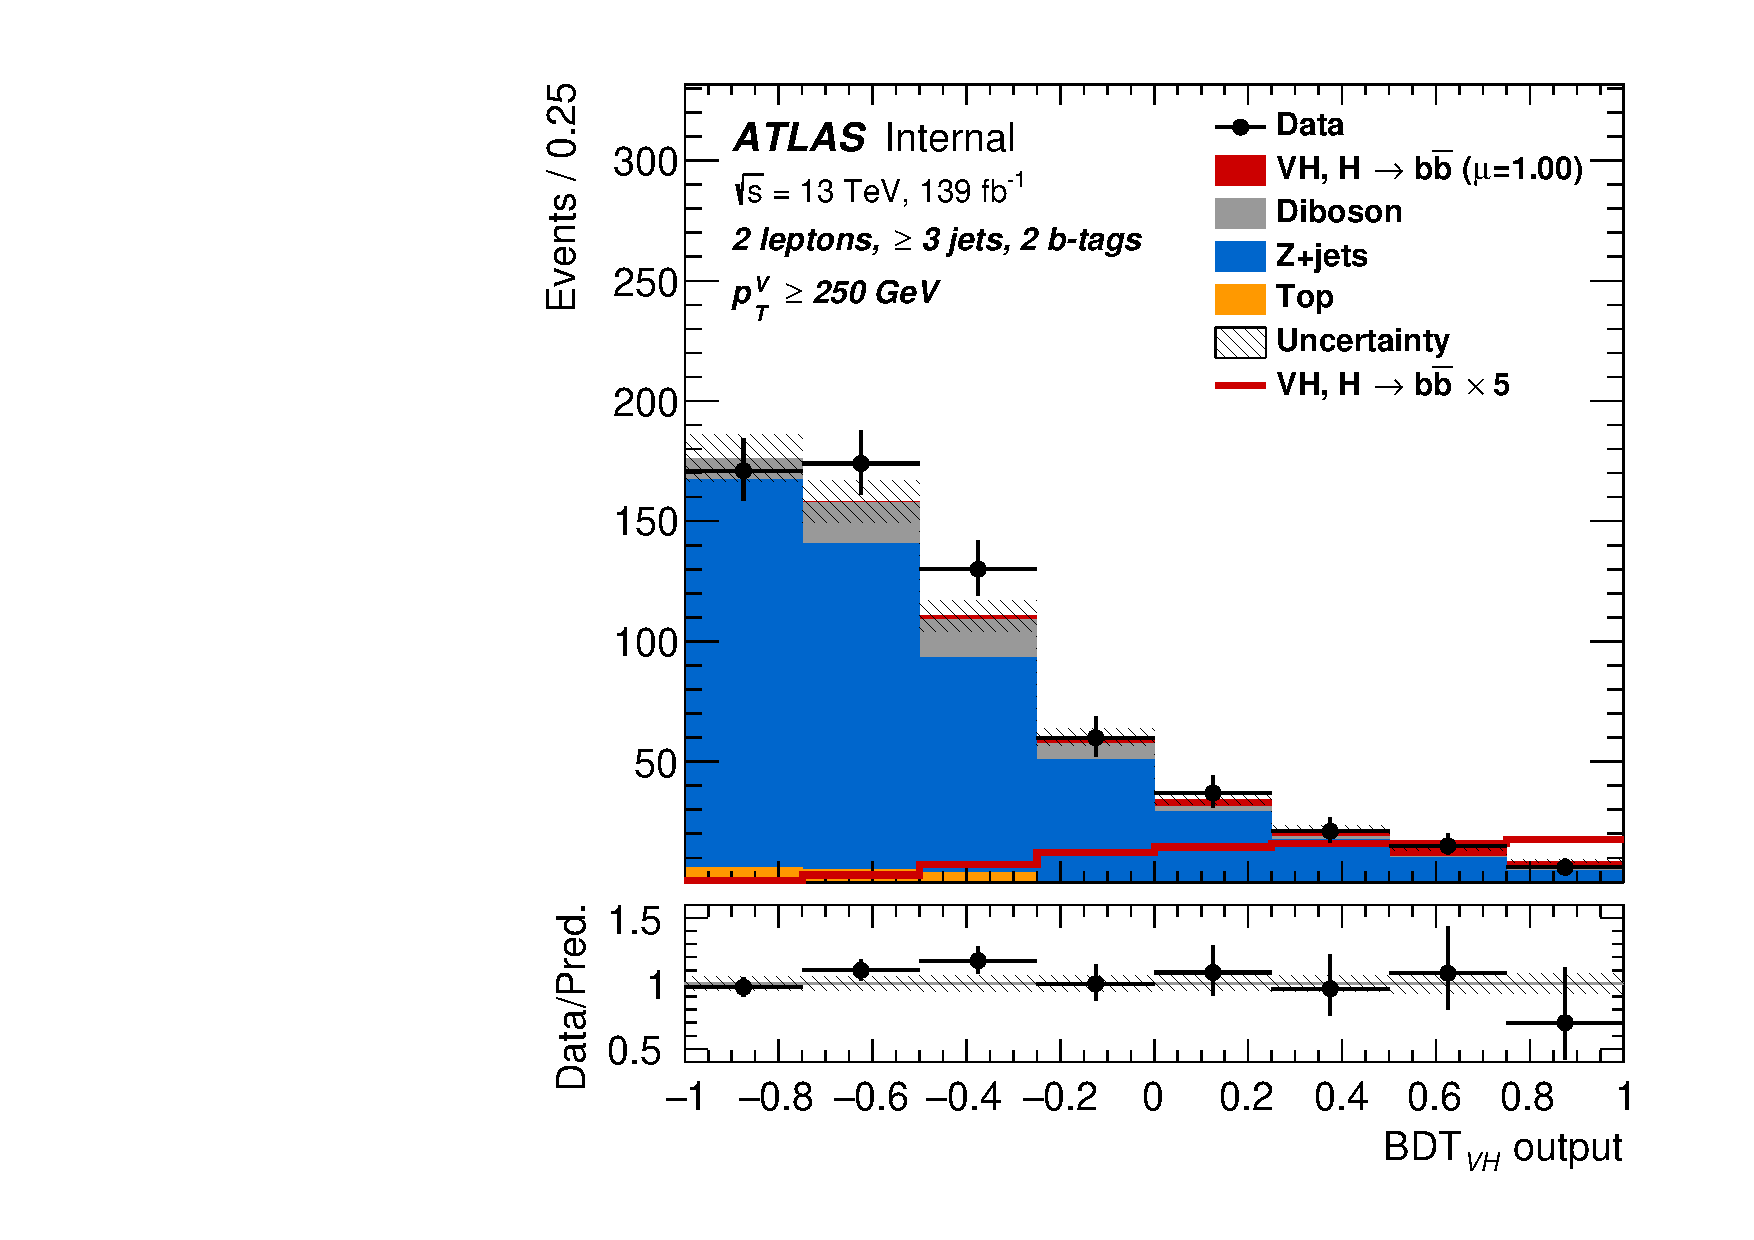
\includegraphics[width=.49\textwidth]{final_fit_mva/prefit/Region_BMin250_incJet1_Y6051_DSR_T2_L2_distmva_J3_Prefit} \\
  \end{tabular}
  \caption{Pre-fit distributions in the signal region of the 2--lepton channel.}
  \label{fig:2lep-sr-prefit}
\end{figure}
\clearpage
\newpage

\section{Analysis Cross-checks}

The final elements of the analysis strategy are a series of cross-checks that
are designed to ensure the methodology is robust. Firstly there is the di-jet
mass fit, also known as the $m_{bb}$ fit. This cross-check is designed to ensure
that the multi-variate analysis has not introduced any biases that have changed
the result so much that is statistically incompatible with a version of the
analysis that does not use the BDT. This cross-check is performed by simply
taking the $m_{bb}$ distribution in place of the BDT distribution in the
profile-likelihood fit.

The second cross-check is a measurement of the diboson process. Diboson final
states arising from proton-proton collisions are well understood and in this
case are being treated as a standard candle\footnote{A standard candle is an
astronomical object with a known absolute luminosity that can be used to aid
astronomical measurements. }. The rationale here is that if the analysis
methodology produces a measurement of the diboson process that is in agreement
with the Standard Model prediction, and therefore existing measurements, then
the methodology itself has not introduced unexpected effects on the result.
Results of these cross-checks imply both of these tests have been
passed~\cite{VHMainNote2019}.

